% **************************************************************************************************************
% A Classic Thesis Style
% An Homage to The Elements of Typographic Style
%
% Copyright (C) 2010 Andr� Miede http://www.miede.de
%
% If you like the style then I would appreciate a postcard. My address 
% can be found in the file ClassicThesis.pdf. A collection of the 
% postcards I received so far is available online at 
% http://postcards.miede.de
%
% License:
% This program is free software; you can redistribute it and/or modify
% it under the terms of the GNU General Public License as published by
% the Free Software Foundation; either version 2 of the License, or
% (at your option) any later version.
%
% This program is distributed in the hope that it will be useful,
% but WITHOUT ANY WARRANTY; without even the implied warranty of
% MERCHANTABILITY or FITNESS FOR A PARTICULAR PURPOSE.  See the
% GNU General Public License for more details.
%
% You should have received a copy of the GNU General Public License
% along with this program; see the file COPYING.  If not, write to
% the Free Software Foundation, Inc., 59 Temple Place - Suite 330,
% Boston, MA 02111-1307, USA.
%
% **************************************************************************************************************
% Note:
%    * You must not use "u etc. in strings/commands that will be spaced out (use \"u or real umlauts instead)
%    * New enumeration (small caps): \begin{aenumerate} \end{aenumerate}
%    * For margin notes: \graffito{}
%    * Do not use bold fonts in this style, it is designed around them
%    * Use tables as in the examples
%    * See classicthesis-ldpkg.sty for useful commands
% **************************************************************************************************************
% To Do:
%    * [high] Check this out: http://www.golatex.de/koma-script-warnung-in-verbindung-mit-listings-package-t2058.html
%    * [medium] mathbb in section-titles/chapter-titles => disappears somehow in headlines!!!
%    * [low] Calculate text block size for Libertine font
%    * [low] Think about processing a4paper, a5paper, 10pt, 11pt, 12pt etc. options for typearea layout
%            (store values in internal variables and handle by \AtEndOfPackage{\areaset...})
% **************************************************************************************************************
\documentclass[ twoside,openright,titlepage,fleqn,numbers=noenddot,headinclude,%1headlines,footinclude
                11pt,letterpaper,BCOR5mm,cleardoublepage=empty,abstractoff % <--- obsolete, remove (todo)
                ]{scrreprt}

% ********************************************************************
% Development Stuff
% ********************************************************************
\listfiles
%\usepackage[l2tabu, orthodox, abort]{nag}
%\usepackage[warning, all]{onlyamsmath}
% ********************************************************************
% Re-usable information
% ********************************************************************
\newcommand{\myTitle}{A Substrate for Accountable Layered Systems\xspace}
\newcommand{\myDegree}{Ph.D. in the Media Arts and Sciences\xspace}
\newcommand{\myName}{Bo Morgan\xspace}
\newcommand{\myProf}{Marvin Minsky\xspace}
\newcommand{\myOtherProf}{Gerald Sussman\xspace}
\newcommand{\mySupervisor}{Joseph Paradiso\xspace}
\newcommand{\myFaculty}{Put data here\xspace}
\newcommand{\myDepartment}{Media Laboratory\xspace}
\newcommand{\myUni}{\protect{Massachusetts Institute of Technology}\xspace}
\newcommand{\myLocation}{Cambridge\xspace}
\newcommand{\myTime}{August 2011\xspace}
\newcommand{\myVersion}{Version 0.1\xspace}
%*******************************************************
% Packages with options that might require adjustments
%*******************************************************
\usepackage[latin1]{inputenc}
\usepackage[ngerman,american]{babel}
\usepackage{natbib}
%\usepackage[square,numbers]{natbib}
\usepackage[fleqn]{amsmath} % math environments and more by the AMS

%*******************************************************
\usepackage{classicthesis-ldpkg} % [backref]
%*******************************************************
% Options for classicthesis.sty:
% tocaligned eulerchapternumbers drafting linedheaders listsseparated 
% subfig nochapters beramono eulermath parts minionpro pdfspacing 
% listings dottedtoc minionprospacing manychapters
\usepackage[eulerchapternumbers,drafting,listings,listsseparated,%pdfspacing,%listings,
            subfig,beramono,eulermath,parts]{classicthesis}

%*******************************************************
% Some font experiments
%*******************************************************
%\usepackage[osf]{libertine}
%\usepackage{hfoldsty}
%\usepackage[light,condensed,math]{iwona}
%\renewcommand{\sfdefault}{iwona}
%\usepackage{lmodern} % <-- no osf support :-(
%\usepackage[urw-garamond]{mathdesign} <-- no osf support :-(

%*******************************************************
% Fine-tuning for the text area
%*******************************************************
%\linespread{1.05} % a bit more for Palatino
%\areaset[5mm]{312pt}{761pt} % 686 (factor 2.2) + 33 head + 42 head \the\footskip
%\setlength{\marginparwidth}{7em}%
%\setlength{\marginparsep}{2em}%

%*******************************************************
% hack to use citations in float environments 
% will be fixed with caption package version 3.2
%*******************************************************
\usepackage{makerobust} 
\makeatletter 
%\MakeRobustCommand\caption@xref 
\makeatother 


% BEGIN DRAFT WATERMARK CODE
%
% This code is from
% http://filoxus.blogspot.com/2008_01_01_archive.html
%
% Thanks to the ``Daily rant: A random blog about everything, mostly
% programming''

\usepackage{graphicx}
\usepackage{type1cm}
\usepackage{eso-pic}
\usepackage{color}

\makeatletter
\AddToShipoutPicture{%
            \setlength{\@tempdimb}{.5\paperwidth}%
            \setlength{\@tempdimc}{.5\paperheight}%
            \setlength{\unitlength}{1pt}%
            \put(\strip@pt\@tempdimb,\strip@pt\@tempdimc){%
        \makebox(0,0){\rotatebox{45}{\textcolor[gray]{0.75}%
        {\fontsize{6cm}{6cm}\selectfont{DRAFT}}}}%
            }%
}
\makeatother

% END DRAFT WATERMARK CODE


%*******************************************************            
%\usepackage[section,below]{placeins} <--- not everybody wants this
%\usepackage[all]{hypcap} <--- does not work with MiKTeX 2.6
% ********************************************************************
% Language/strings for backrefs (change here, thanks, Lorenzo)
%*******************************************************
%\renewcommand{\backrefnotcitedstring}{\relax}%(Not cited.)
%\renewcommand{\backrefcitedsinglestring}[1]{(Citato a pagina~#1.)}
%\renewcommand{\backrefcitedmultistring}[1]{(Citato alle pagine~#1.)}
%\renewcommand{\backreftwosep}{ e~}
%\renewcommand{\backreflastsep}{ e~}
% ********************************************************************
% Setup and Finetuning
%*******************************************************
\newlength{\abcd} % for ab..z string length calculation
\newcommand{\myfloatalign}{\centering} % how all the floats will be aligned
\setlength{\extrarowheight}{3pt} % increase table row height
% ********************************************************************
% Captions look and feel
%*******************************************************
\captionsetup{format=hang,font=small}
% ********************************************************************
% Listings setup
% ********************************************************************
%\lstset{emph={trueIndex,root},emphstyle=\color{BlueViolet}}%\underbar} % for special keywords
% ********************************************************************
\lstset{language=[LaTeX]Tex,%C++,
    keywordstyle=\color{RoyalBlue},%\bfseries,
    basicstyle=\small\ttfamily,
    %identifierstyle=\color{NavyBlue},
    commentstyle=\color{Green}\ttfamily,
    stringstyle=\rmfamily,
    numbers=none,%left,%
    numberstyle=\scriptsize,%\tiny
    stepnumber=5,
    numbersep=8pt,
    showstringspaces=false,
    breaklines=true,
    frameround=ftff,
    frame=single,
    belowcaptionskip=.75\baselineskip,
    %numberbychapter=false
    %frame=L
} 

% ********************************************************************
% Where to look for graphics
%*******************************************************
%\graphicspath{{gfx/}{misc/}} % considered harmful according to l2tabu
% ********************************************************************
% Hyperreferences
%*******************************************************
\hypersetup{%
    colorlinks=true, linktocpage=true, pdfstartpage=3, pdfstartview=FitV,%
    % uncomment the following line if you want to have black links (e.g., for printing)
    %colorlinks=false, linktocpage=false, pdfborder={0 0 0}, pdfstartpage=3, pdfstartview=FitV,% 
    breaklinks=true, pdfpagemode=UseNone, pageanchor=true, pdfpagemode=UseOutlines,%
    plainpages=false, bookmarksnumbered, bookmarksopen=true, bookmarksopenlevel=1,%
    hypertexnames=true, pdfhighlight=/O,%hyperfootnotes=true,%nesting=true,%frenchlinks,%
    urlcolor=webbrown, linkcolor=RoyalBlue, citecolor=webgreen, %pagecolor=RoyalBlue,%
    %urlcolor=Black, linkcolor=Black, citecolor=Black, %pagecolor=Black,%
    pdftitle={\myTitle},%
    pdfauthor={\textcopyright\ \myName, \myUni, \myFaculty},%
    pdfsubject={},%
    pdfkeywords={},%
    pdfcreator={pdfLaTeX},%
    pdfproducer={LaTeX with hyperref and classicthesis}%
}

%********************************************************************
% Hyphenation
%*******************************************************
%\hyphenation{put special hyphenation here}
% ********************************************************************
% GO!GO!GO! MOVE IT!
%*******************************************************
\begin{document}
\frenchspacing
\raggedbottom
\selectlanguage{american} % american ngerman
%\renewcommand*{\bibname}{new name}
%\setbibpreamble{}
\pagenumbering{roman}
\pagestyle{plain}
%********************************************************************
% Frontmatter
%*******************************************************
%*******************************************************
% Little Dirty Titlepage
%*******************************************************
\thispagestyle{empty}
%\pdfbookmark[1]{Titel}{title}
%*******************************************************
\begin{center}
    \spacedlowsmallcaps{\myName} \\ \medskip                        

    \begingroup
        \color{Maroon}\spacedallcaps{\myTitle}
    \endgroup
\end{center}        

\makebox[7in]{
  {\flushright{Advisor\hspace{0.5cm}          \makebox[3in]{\hrulefill}}}
  
  {\flushright{Committee Member\hspace{0.5cm} \makebox[3in]{\hrulefill}}}
}

%*******************************************************
% Titlepage
%*******************************************************
\begin{titlepage}
	% if you want the titlepage to be centered, uncomment and fine-tune the line below (KOMA classes environment)
	\begin{addmargin}[-1cm]{-3cm}
    \begin{center}
        \large  

        \hfill

        \vfill

        \begingroup
            \color{Maroon}\spacedallcaps{\myTitle} \\ \bigskip
        \endgroup

        \spacedlowsmallcaps{\myName}

        \vfill

        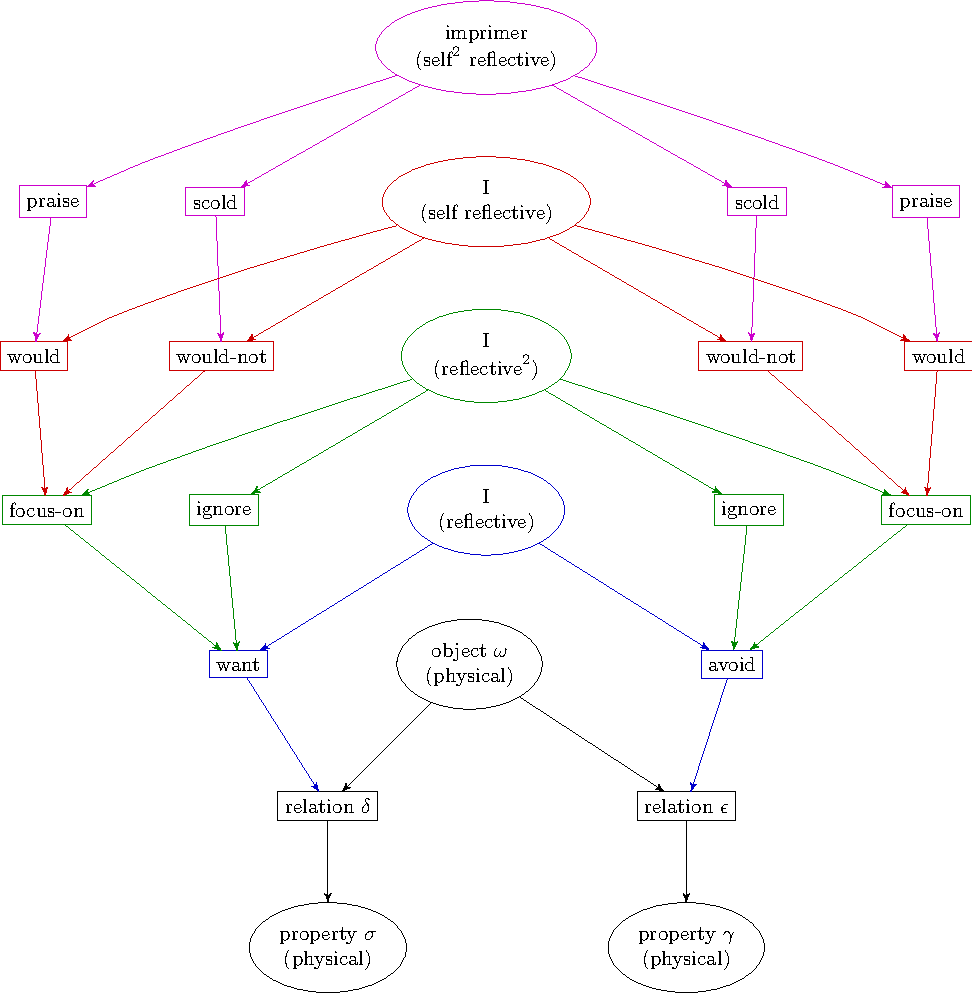
\includegraphics[width=4cm]{gfx/model-6} \\ \medskip

        \myDegree \\ \medskip   
        %\myDepartment \\                            
        %\myFaculty \\
        %\myUni \\ \bigskip

        \myTime

        \vfill                      

    \end{center}  
  \end{addmargin}       
\end{titlepage}   

\thispagestyle{empty}

\hfill

\vfill

\noindent\myName: \textit{\myTitle,} \myDegree, \textcopyright\ \myTime

%\bigskip
%
%\noindent\spacedlowsmallcaps{Supervisors}: \\
%\myProf \\
%\myOtherProf \\ 
%\mySupervisor
%
%\medskip
%
%\noindent\spacedlowsmallcaps{Location}: \\
%\myLocation
%
%\medskip
%
%\noindent\spacedlowsmallcaps{Time Frame}: \\
%\myTime

\cleardoublepage%*******************************************************
% Dedication
%*******************************************************
\thispagestyle{empty}
%\phantomsection 
\refstepcounter{dummy}
\pdfbookmark[1]{Dedication}{Dedication}

\vspace*{3cm}

%\begin{center}
%``If wishes were horses, beggars would ride.''  Since they are not, \\ \medskip
%since really to satisfy an impulse or interest means to work it out, \\ \medskip
%and working it out involves running up against obstacles, \\ \medskip
%becoming acquainted with materials, exercising ingenuity, \\ \medskip
%patience, persistence, alertness, it of necessity involves \\ \medskip
%discipline---ordering of power and supplies knowledge. \\ \medskip
%    --- \defcitealias{dewey:1907}{John Dewey}\citetalias{dewey:1907}
%\end{center}
%
%\medskip

%
%Though there be no such thing as Chance in the world; \\
%our ignorance of the real cause of any event \\
%has the same influence on the understanding, \\
%and begets a like species of belief or opinion.} \\ \medskip
%    --- \defcitealias{hume:1902}{David Hume}\citetalias{hume:1902}
%
%
%

\begin{center}
Though there be no such thing as Chance in the world; \\
our ignorance of the real cause of any event \\
has the same influence on the understanding, \\
and begets a like species of belief or opinion. \\ \medskip
    --- \defcitealias{hume:1902}{David Hume}\citetalias{hume:1902}
\end{center}

\medskip

\begin{center}
    Dedicated to the loving memory of Pushpinder Singh. \\ \smallskip
    1972\,--\,2006
\end{center}

\cleardoublepage%*******************************************************
% Abstract
%*******************************************************
%\renewcommand{\abstractname}{Abstract}
\pdfbookmark[1]{Abstract}{Abstract}
\begingroup
\let\clearpage\relax
\let\cleardoublepage\relax
\let\cleardoublepage\relax

\chapter*{Abstract}

There have been two directions of research with the goal of building a
machine that explains intelligent human behavior.  The first approach
is to build a baby-machine that learns from scratch to accomplish
goals through interactions with its environment.  The second approach
is to give the machine an abundance of knowledge that represents
correct behavior.

Each of these solutions has benefits and drawbacks.  The baby-machine
approach is good for dealing with novel problems, but these problems
are necessarily simple because complex problems require a lot of
background knowledge.  The data abundance approach deals well with
complicated problems requiring a lot of background knowledge, but
fails to adapt to changing environments, for which the algorithm has
not already been trained.

We are working on an algorithm that benefits from both of these
approaches by learning from cultural language knowledge, while
reflectively monitoring and recognizing the failures of this knowledge
when it is used in a goal-oriented domain.

Toward this end we have developed a reflective programming language
allowing us the ability to monitor the execution and interactions
between large numbers of complicated lisp-like processes.  Further, we
have developed a cognitive architecture within our language that
provides structures for layering reflective processes, resulting in a
hierarchy of control algorithms that respond to failures in the layers
below.

Finally, we present an example of our cognitive architecture learning
in the context of a social commonsense reasoning domain with parents
that teach children as they attempt to accomplish cooking tasks in a
kitchen.

\endgroup

\vfill

\cleardoublepage%*******************************************************
% Publications
%*******************************************************
\pdfbookmark[1]{Publications}{publications}
\chapter*{Publications}
Some ideas and figures have appeared previously in the following publications:

\bigskip

\noindent Smith, D. and Morgan, B.; "IsisWorld: An open source
 commonsense simulator for AI researchers"; AAAI 2010 Workshop on
 Metacognition; 2010 April

\vspace{5mm}

\noindent Morgan, B.; ``Moral Compass: Commonsense Social Reasoning
 Cognitive Architecture''; http://em-two.net/about; Commonsense Tech
 Note; MIT Media Lab; 2011 January

\vspace{5mm}

\noindent Morgan, B.; ``A Computational Theory of the Communication of
 Problem Solving Knowledge between Parents and Children''; PhD
 Proposal; MIT Media Lab 2010 January

\vspace{5mm}

\noindent Morgan, B.; ``Funk2: A Distributed Processing Language for 
 Reflective Tracing of a Large Critic-Selector Cognitive
 Architecture''; Proceedings of the Metacognition Workshop at the
 Third IEEE International Conference on Self-Adaptive and
 Self-Organizing Systems; San Francisco, California, USA; 2009
 September

\vspace{5mm}

\noindent Morgan, B.; ``Funk2: A Frame-based Programming Language with
 Causally Reflective Capabilities (draft in progress)''; Technical
 Note; Massachusetts Institute of Technology; 2009 May

\vspace{5mm}

\noindent Morgan, B.; ``Learning Commonsense Human-language Descriptions
 from Temporal and Spatial Sensor-network Data''; Masters Thesis;
 Massachusetts Institute of Technology; 2006 August

\vspace{5mm}

\noindent Morgan, B.; ``Learning perception lattices to compare
 generative explanations of human-language stories''; Published
 Online; Commonsense Tech Note; MIT Media Lab; 2006 July

\vspace{5mm}

\noindent Morgan, B. and Singh, P.; ``Elaborating Sensor Data using
 Temporal and Spatial Commonsense Reasoning''; International Workshop
 on Wearable and Implantable Body Sensor Networks (BSN-2006); 2005
 November

\vspace{5mm}

\noindent Morgan, B.; ``Experts think together to solve hard problems'';
 Published Online; Commonsense Tech Note; MIT Media Lab 2005 August

\vspace{5mm}

\noindent Morgan, B.; ``LifeNet Belief Propagation''; Published Online;
 Commonsense Tech Note; MIT Media Lab; 2004 January

\cleardoublepage%*******************************************************
% Acknowledgments
%*******************************************************
\pdfbookmark[1]{Acknowledgments}{acknowledgments}

%Don't do anything that isn't play. \\ \medskip
%    --- Joseph Campbell



\begin{flushright}{\slshape    
Don't do anything that isn't play.} \\ \medskip
    --- Joseph Campbell
\end{flushright}



\bigskip

\begingroup
\let\clearpage\relax
\let\cleardoublepage\relax
\let\cleardoublepage\relax
\chapter*{Acknowledgments}

I would first like to thank:

\begin{itemize}
\item{Push Singh for being a good friend and advisor.}
\end{itemize}

Next I would like to thank my committee:

\begin{itemize}
\item{Joe Paradiso for unfailing support and faith in my ability to do
  something well.}
\item{Marvin Minsky for consistently and patiently providing an
  inspiringly critical perspective and a wealth of important problems
  to solve.}
\item{Gerry Sussman for loving to program.}
\item{Mike Cox for providing critical direction for navigating the
  space of the contemporary meta-cognitive computational sciences.}
\end{itemize}

I would next like to thank my immediate family:

\begin{itemize}
\item{Greg Morgan and Carolyn Spinner for being supportive parents---willing to help me think about anything at any time.}
\item{Paul Bergman for teaching me how to program.}
\item{Virginia Barasch for painting my finger nails.}
\item{Leaf Morgan for playing Archon with me.}
\end{itemize}

Professors:

\begin{itemize}
\item{Henry Lieberman}
\item{Ed Boyden}
\item{Walter Bender}
\item{Ted Selker}
\end{itemize}

Popes:

\begin{itemize}
\item{Dustin Smith}
\item{Scotty Vercoe}
\item{Dane Scalise}
\end{itemize}

Friends:

\begin{itemize}
\item{Mako Hill}
\item{Barbara Barry}
\end{itemize}

\endgroup


\pagestyle{scrheadings}
\cleardoublepage%*******************************************************
% Table of Contents
%*******************************************************
%\phantomsection
\refstepcounter{dummy}
\pdfbookmark[1]{\contentsname}{tableofcontents}
\setcounter{tocdepth}{2} % <-- 2 includes up to subsections in the ToC
\setcounter{secnumdepth}{3} % <-- 3 numbers up to subsubsections
\manualmark
\markboth{\spacedlowsmallcaps{\contentsname}}{\spacedlowsmallcaps{\contentsname}}
\tableofcontents 
\automark[section]{chapter}
\renewcommand{\chaptermark}[1]{\markboth{\spacedlowsmallcaps{#1}}{\spacedlowsmallcaps{#1}}}
\renewcommand{\sectionmark}[1]{\markright{\thesection\enspace\spacedlowsmallcaps{#1}}}%*******************************************************
% List of Figures and of the Tables
%*******************************************************
\clearpage

\begingroup 
    \let\clearpage\relax
    \let\cleardoublepage\relax
    \let\cleardoublepage\relax
    %*******************************************************
    % List of Figures
    %*******************************************************    
    %\phantomsection 
    \refstepcounter{dummy}
    %\addcontentsline{toc}{chapter}{\listfigurename}
    \pdfbookmark[1]{\listfigurename}{lof}
    \listoffigures

    \vspace*{8ex}

    %*******************************************************
    % List of Tables
    %*******************************************************
    %\phantomsection 
    \refstepcounter{dummy}
    %\addcontentsline{toc}{chapter}{\listtablename}
    \pdfbookmark[1]{\listtablename}{lot}
    \listoftables
        
    \vspace*{8ex}
%   \newpage
    
    %*******************************************************
    % List of Listings
    %*******************************************************      
	  %\phantomsection 
    \refstepcounter{dummy}
    %\addcontentsline{toc}{chapter}{\lstlistlistingname}
    \pdfbookmark[1]{\lstlistlistingname}{lol}
    \lstlistoflistings 

    \vspace*{8ex}
       
    %*******************************************************
    % Acronyms
    %*******************************************************
    %\phantomsection 
    \refstepcounter{dummy}
    \pdfbookmark[1]{Acronyms}{acronyms}
    \markboth{\spacedlowsmallcaps{Acronyms}}{\spacedlowsmallcaps{Acronyms}}
    \chapter*{Acronyms}
    \begin{acronym}[UML]
        \acro{GPS}{General Problem Solver}
    \end{acronym}                     
\endgroup

\cleardoublepage

%*******************************************************
% Mainmatter
%*******************************************************
\pagenumbering{arabic}
\cleardoublepage\part{Introduction}
%************************************************
\chapter{Learning to Accomplish Goals}\label{ch:learning_to_accomplish_goals}
%************************************************

\begin{quote}
  Problem-solvers must find relevant data.  How does the human mind
  retrieve what it needs from among so many millions of knowledge items?
  Different AI systems have attempted to use a variety of different
  methods for this.  Some assign keywords, attributes, or descriptors to
  each item and then locate data by feature-matching or by using more
  sophisticated associative data-base methods.  Others use
  graph-matching or analogical case-based adaptation.  Yet others try to
  find relevant information by threading their ways through systematic,
  usually hierarchical classifications of knowledge---sometimes called
  ``ontologies''.  But, to me, all such ideas seem deficient because it
  is not enough to classify items of information simply in terms of the
  features or structures of those items themselves.  This is because we
  rarely use a representation in an intentional vacuum, but we always
  have goals---and two objects may seem similar for one purpose but
  different for another purpose.
\end{quote}
\begin{flushright}
  --- \defcitealias{minsky:1991}{Marvin Minsky}\citetalias{minsky:1991}
\end{flushright}

% horvat: -^^^
%
%  very true
%  you could disuss it in paralell to the view that “mind
%  is a system always evolving” (Hoya, 2005)
%

In this introductory chapter I will give an overview of the problem of
reflectively learning to accomplish goals.  First, I will develop the
assumption that any process that I choose under given constraints can
be reflectively monitored and useful information, e.g. beginning and
ending times, will be temporarily stored.  In other words, I assume
that my system natively supports procedural reflection for all
processes.  Given this assumption, I show in this chapter that the
problem of building a system that learns to accomplish goals in its
environment becomes a simple loop-less causal structure involving at
least four different types of learning.  These four types of learning
complete a circle of causal learning from goals through actions to
physical states and back to goals, but because of time, causality is
still in an ordered lattice structure beginning with goals as the
causal roots for all other knowledge.

In later chapters I will introduce experiments I have performed in
different physical problem simulations.  The first is a simple
proof-of-concept demonstration of my reflective learning algorithm in
a blocks world problem domain.  Also, I show my reflective
architecture extended to a larger physical reasoning domain, including
multiple agents learning to cook together in a kitchen environment.
In this larger problem space, agents can communicate high-level
procedures specified in a simple programming language that is shared
by the agents, and refers to both mental and physical actions of the
agents.

\section{The Agent-Environment Model}

\begin{figure}[bth]
  \center
  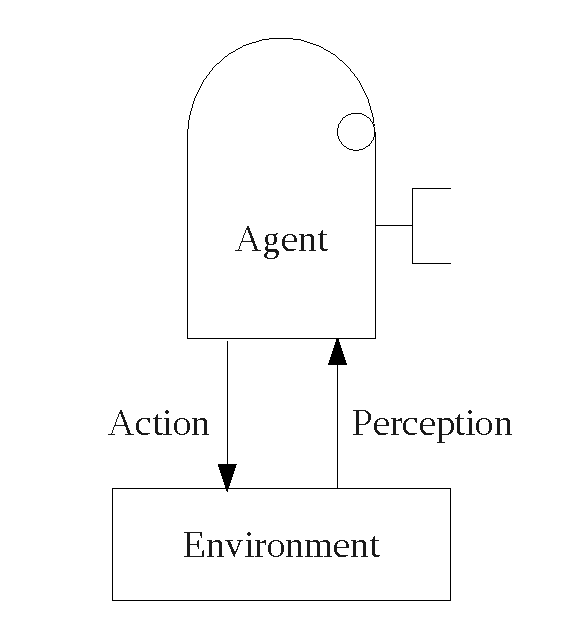
\includegraphics[height=5cm]{gfx/agent_environment}
  \caption[The agent-environment model]{The agent-environment model.}
  \label{fig:agent_environment}
\end{figure}

Figure~\ref{fig:agent_environment} shows the basic agent-environment
model.  In this model, I make a distinction between the environment
and the agent.  At any given time, the agent and the environment are
each represented as a specific static form of data.  Further, these
representations change over time, according to a given transfer
function.  I will treat this system as a deterministic system,
although one could imagine adding random variables to the transfer
function: the basic theory is the same.  It is easier to add
randomness to a deterministic theory than the opposite.  There are
also many benefits to developing a deterministic model with perhaps a
pseudorandom aspect because this allows for the repeatability of
scientific experiments, for which the model may be used as a metric.
The two processes communicate information along two channels: (1) an
action channel from the agent to the environment, and (2) a perception
channel from the environment to the agent.


\section{The State-Action Model}
\label{sec:state_action_model}

\begin{figure}[bth]
  \center
  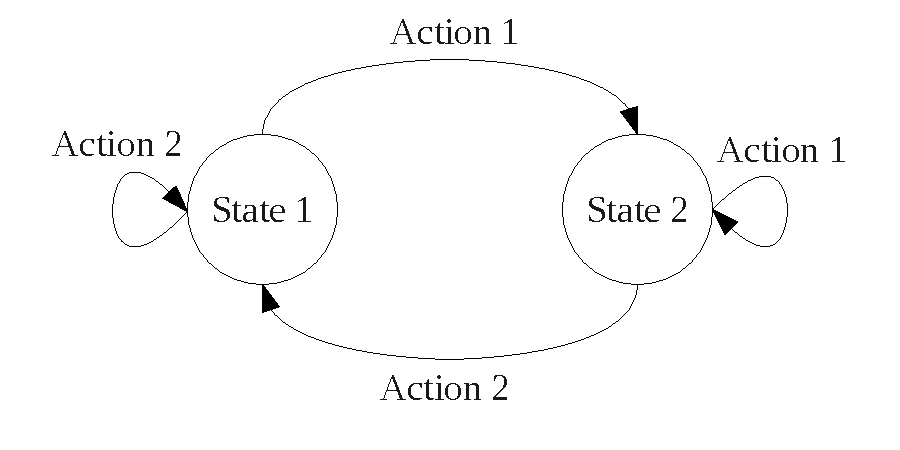
\includegraphics[width=6cm]{gfx/state_action}
  \caption[The state-action model]{The state action model.  Two states
    are represented by nodes and two actions are represented by edges
    from each of the two states.}
  \label{fig:state_action}
\end{figure}

The agent is in an environment, which is in a specific state.  My
agent performs an action, which can affect the state of the
environment.  Figure~\ref{fig:state_action} shows a simple \ac{FSM}
state-action model, which has two states for the environment and two
actions for the agent to perform in each of these states.  The
state-action model is a simple model for how actions map to changes in
the state of the environment.


\section{A Multiple Agent-Environment Model}

\begin{figure}[bth]
  \center
  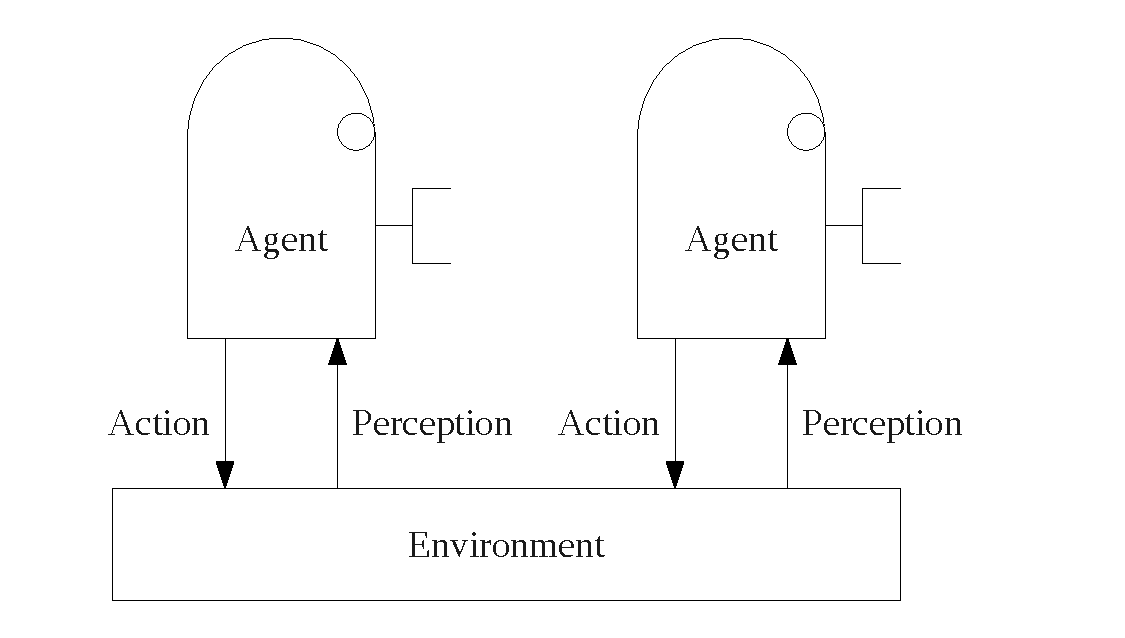
\includegraphics[height=5cm]{gfx/multiple_agent_environment}
  \caption[The multiple agent environment model]{The multiple agent environment model.}
  \label{fig:multiple_agent_environment}
\end{figure}

In order to model social intelligence, we introduce the multiple agent
environment model shown in
Figure~\ref{fig:multiple_agent_environment}.


\section{Agent Process Communication}

Because agent processes can only directly act on and perceive the
environment, all communication between agent processes must occur
through the environment process.  We assume that agents can
communicate some form of symbolic knowledge structure in the absence
of noise.  These representations are used to communicate processes
from one agent to another.  Specific examples of such a process
representation that we have used in our experiments are described in
more detail in
Sections~\ref{sec:serial_process_representation}--\ref{sec:parallel_process_representation}.


\section{A Relational State Representation}

\begin{figure}[bth]
  \center
  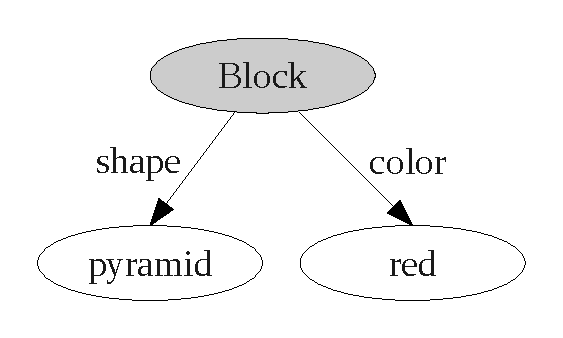
\includegraphics[height=3cm]{gfx/frame_representation}
  \caption[Frame-based relational representation]{Frame-based relational representation.}
  \label{fig:frame_representation}
\end{figure}

See Figure~\ref{fig:frame_representation}.

\section{Introducing Reflection Early in the Process}

Now, I have introduced my problem as being divided into at least two
processes, at least one agent process and an environment process.
Further, I have introduced how a basic process may be thought of as an
\ac{FSM}.  At this point, I introduce a model for keeping track of the
changes in a computational process: reflective knowledge.  I
purposefully make this assumption before I define the details of the
agent model process because, in my approach, I would like to
reflectively reason about potentially any aspect of this agent
process.

\section{Reflective Knowledge}

\begin{figure}[bth]
  \center
  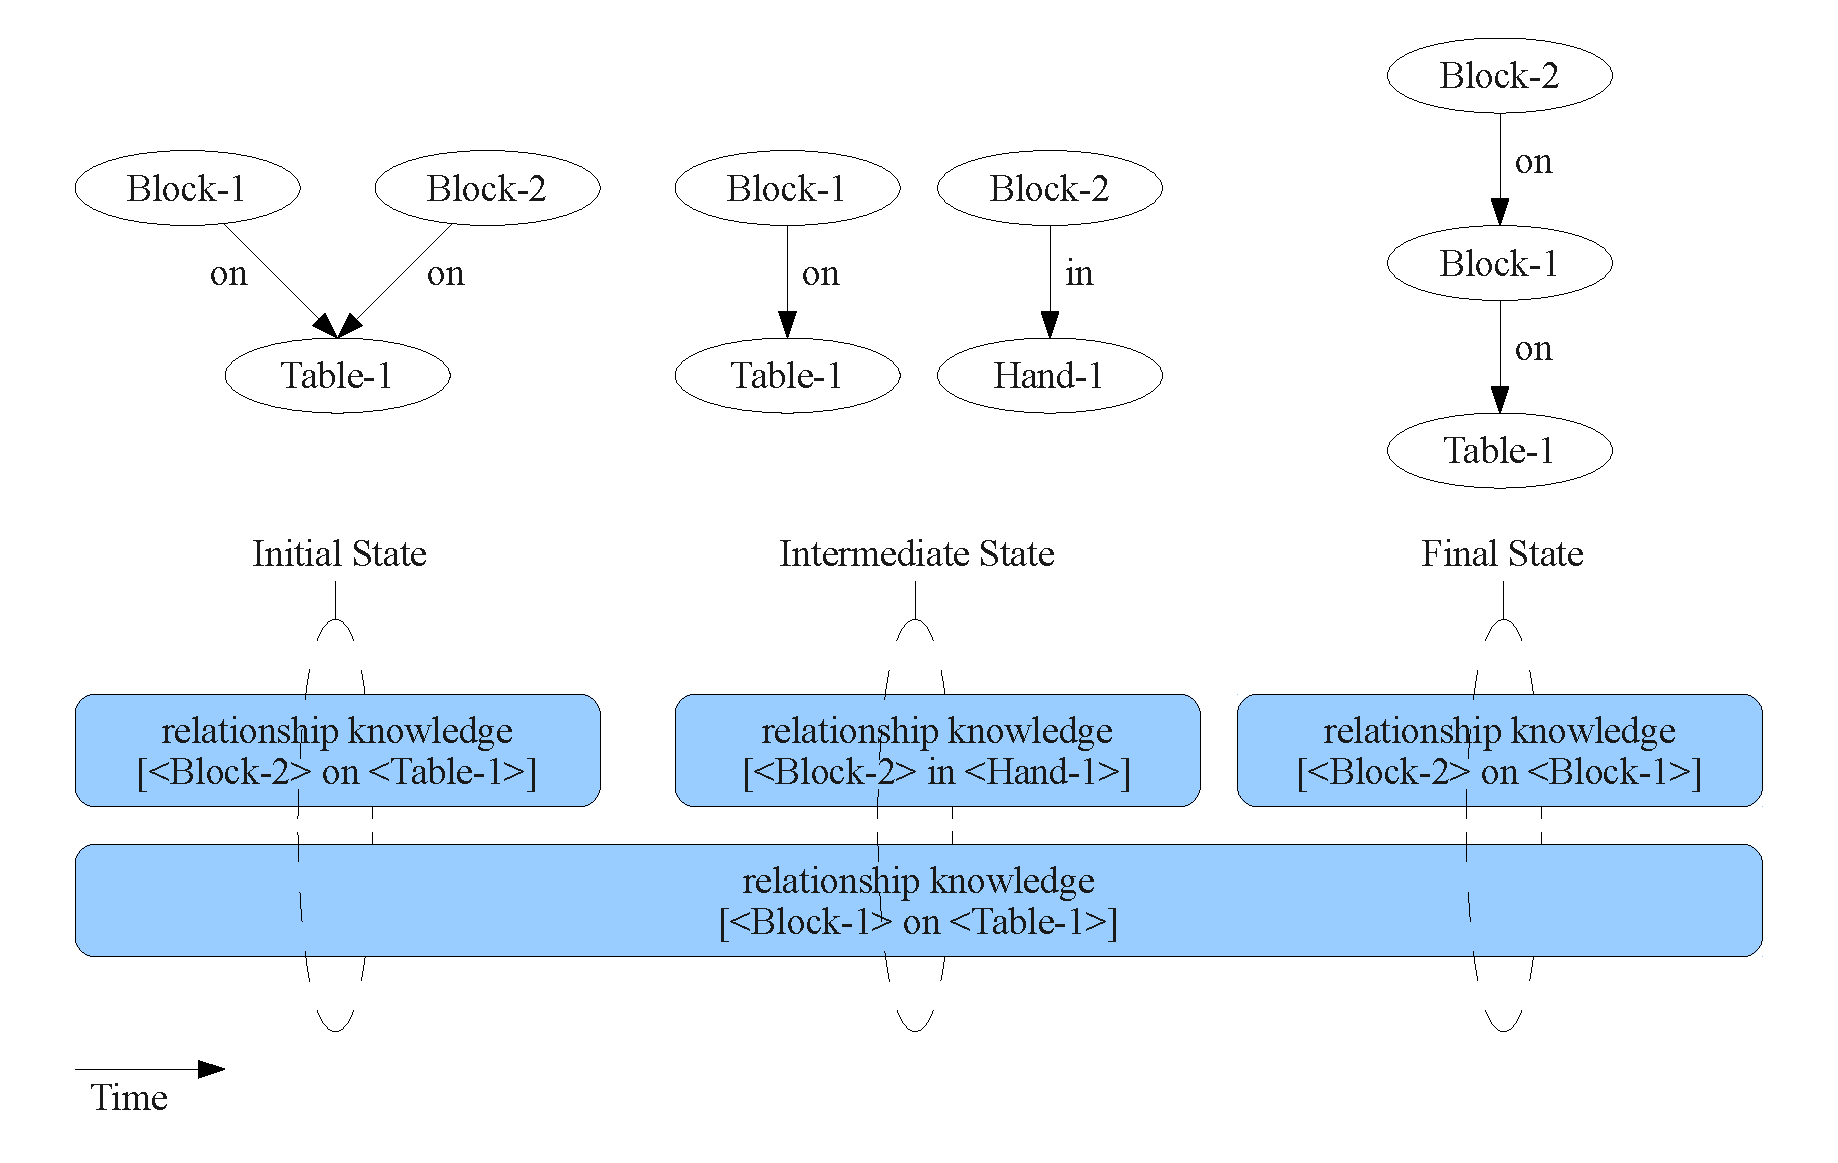
\includegraphics[width=12cm]{gfx/reflective_event_representation}
  \caption[A reflective event representation]{A reflective event representation shows the changes in a labeled graph.}
  \label{fig:reflective_event_representation}
\end{figure}


While the term meta-knowledge is used to describe the very general
idea of knowledge about knowledge, I use the term reflective knowledge
to refer to the specific type of meta-knowledge that refers to
knowledge about the changes to a knowledge structure.  If I keep track
of the changes to a knowledge structure, I can later integrate these
changes in order to obtain an equivalent form of that knowledge
structure as it was at any point in the past.\footnote{See
  Section~\ref{sec:what_is_a_computer} for a discussion of more
  realistic models of computation, including multiple-core and cluster
  models.}




\section{Frame Perceptions}

\begin{figure}[bth]
  \center
  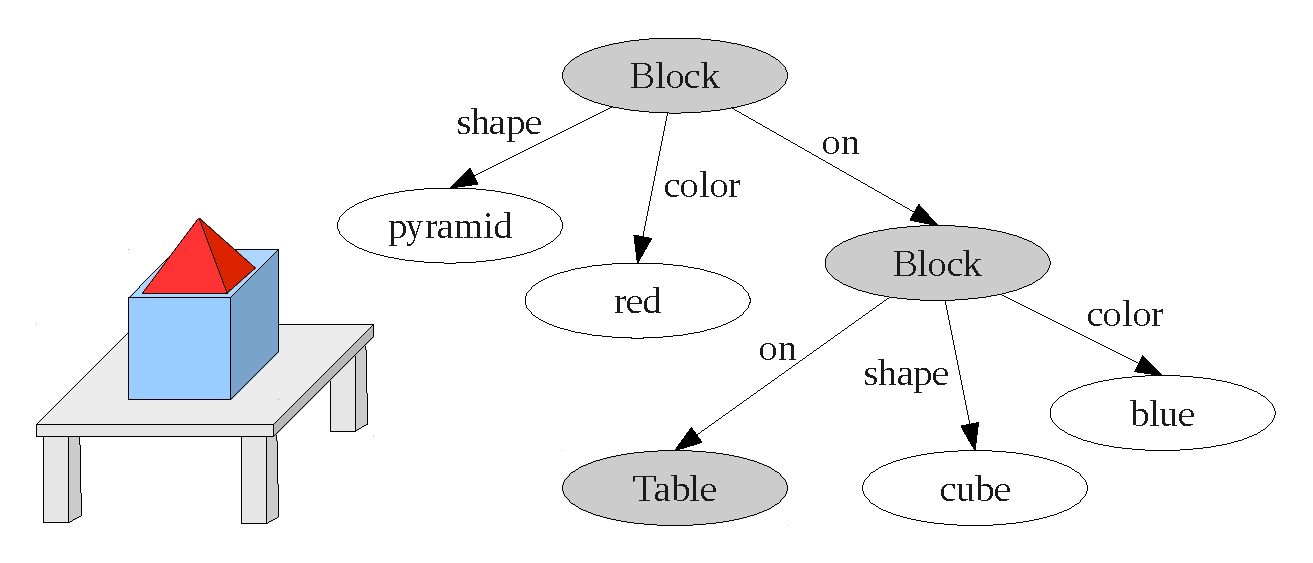
\includegraphics[height=5cm]{gfx/frame_perception}
  \caption[Collections of frames used as perceptual input to agent]{Collections of frames used as perceptual input to agent.}
  \label{fig:frame_perception}
\end{figure}

See Figure~\ref{fig:frame_perception}.


\section{Partially Observable State Model}

\begin{figure}[bth]
  \center
  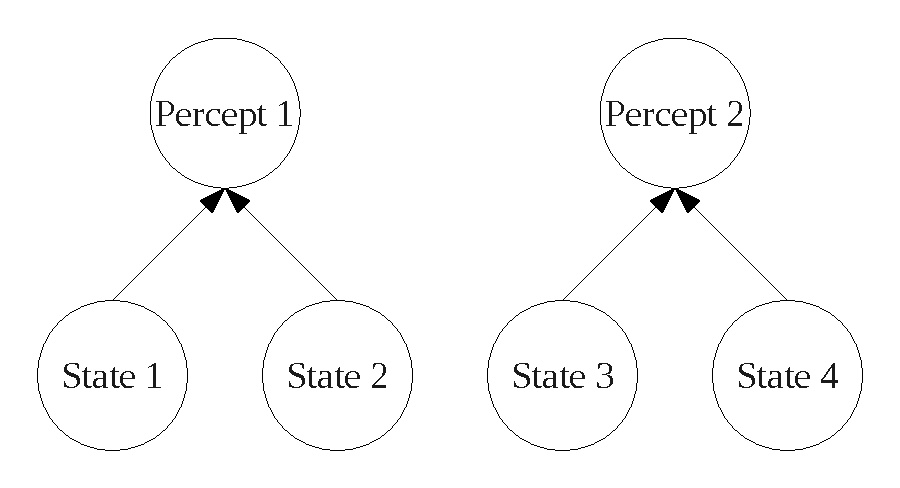
\includegraphics[width=6cm]{gfx/partially_observable}
  \caption[The partially observable state model]{The partially observable model.}
  \label{fig:partially_observable}
\end{figure}

\begin{figure}[bth]
  \center
  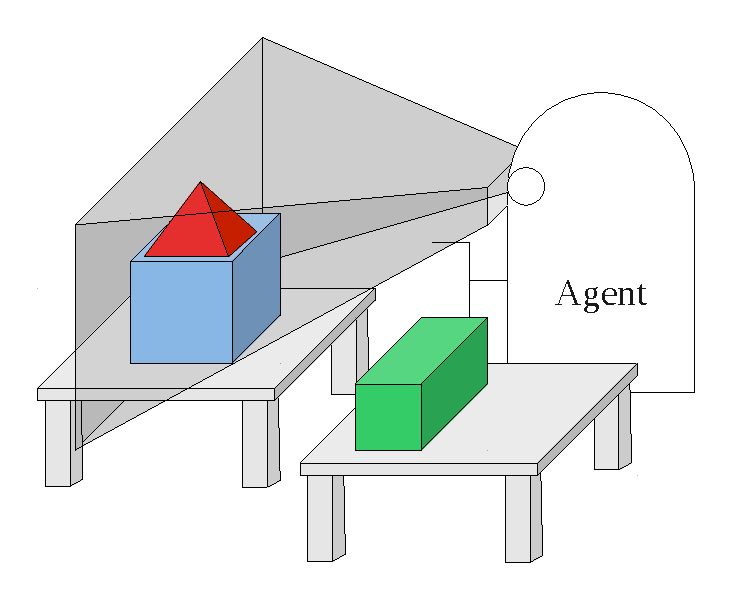
\includegraphics[height=5cm]{gfx/partial_frame_perception}
  \caption[The state of the environment is only partially
    observable]{The state of the environment is only partially
    observable.}
  \label{fig:partial_frame_perception}
\end{figure}

The agent process does not have complete access to the state of its
environment.  The agent's perceptual stream of information depends on
the state of the environment, but it is a function of the environment
and not the actual state of the environment.  In other words, the
perceptual state that is communicated from the environment to the
agent is an injective function mapping the environment to the
perception of the agent.  See
Figures~\ref{fig:partially_observable}~and~\ref{fig:partial_frame_perception}
for two examples of partially observable environments.


\section{Agent Abstract Physical Model}

\begin{figure}[bth]
  \center
  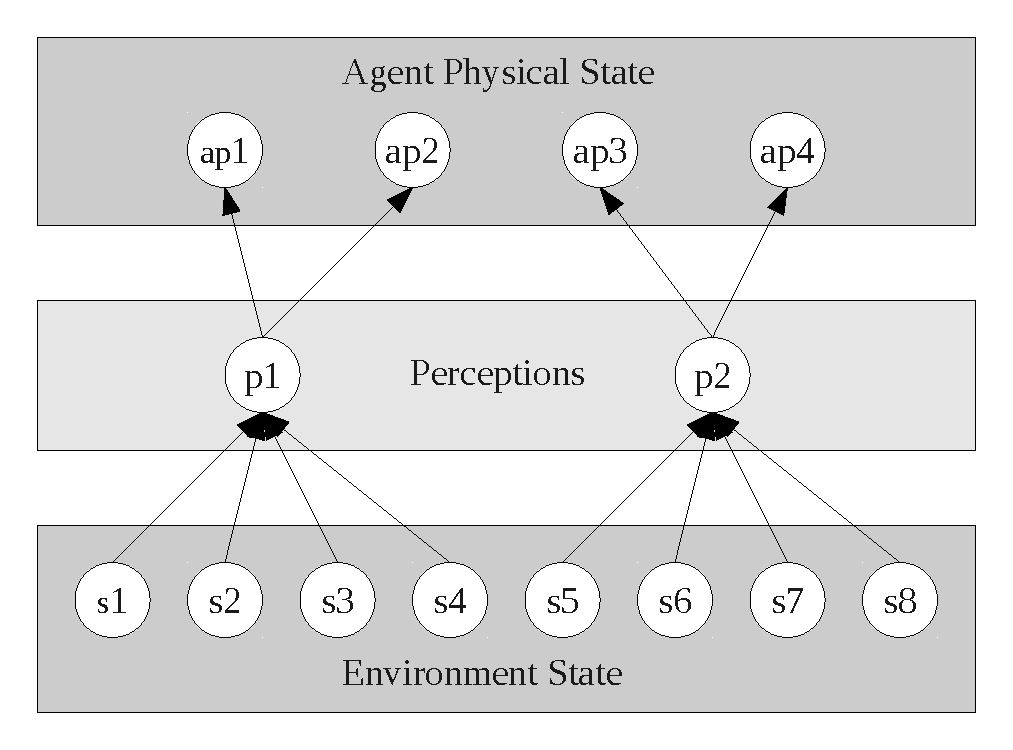
\includegraphics[width=8cm]{gfx/environment_perception_physical}
  \caption[The agent has an abstract physical model of the
    environment]{The agent has an abstract physical model of the
    environment.}
  \label{fig:environment_perception_physical}
\end{figure}

See Figure~\ref{fig:environment_perception_physical}.


\section{A Physical Goal Representation}

\begin{figure}[bth]
  \center
  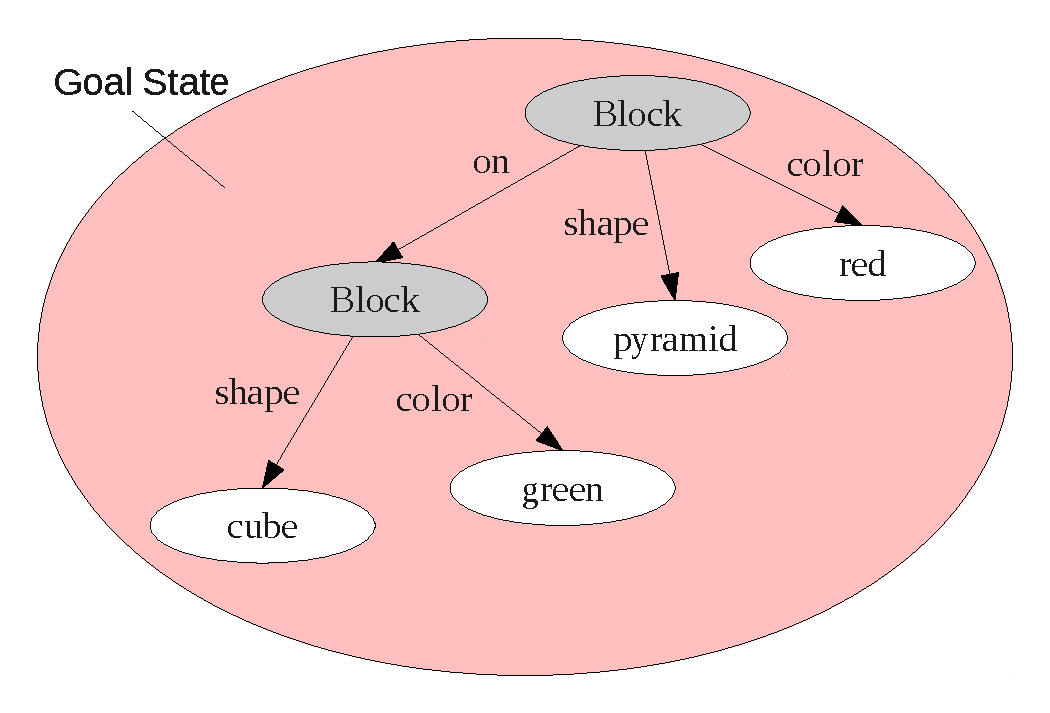
\includegraphics[height=4cm]{gfx/goal_state}
  \caption[A physical goal representation]{A physical goal
    representation is a structural relationship that may or may not
    currently exist within the physical knowledge base.}
  \label{fig:goal_state}
\end{figure}

See Figure~\ref{fig:goal_state}.


\section{The Reflective Learning Cycle}

\begin{figure}[bth]
  \center
  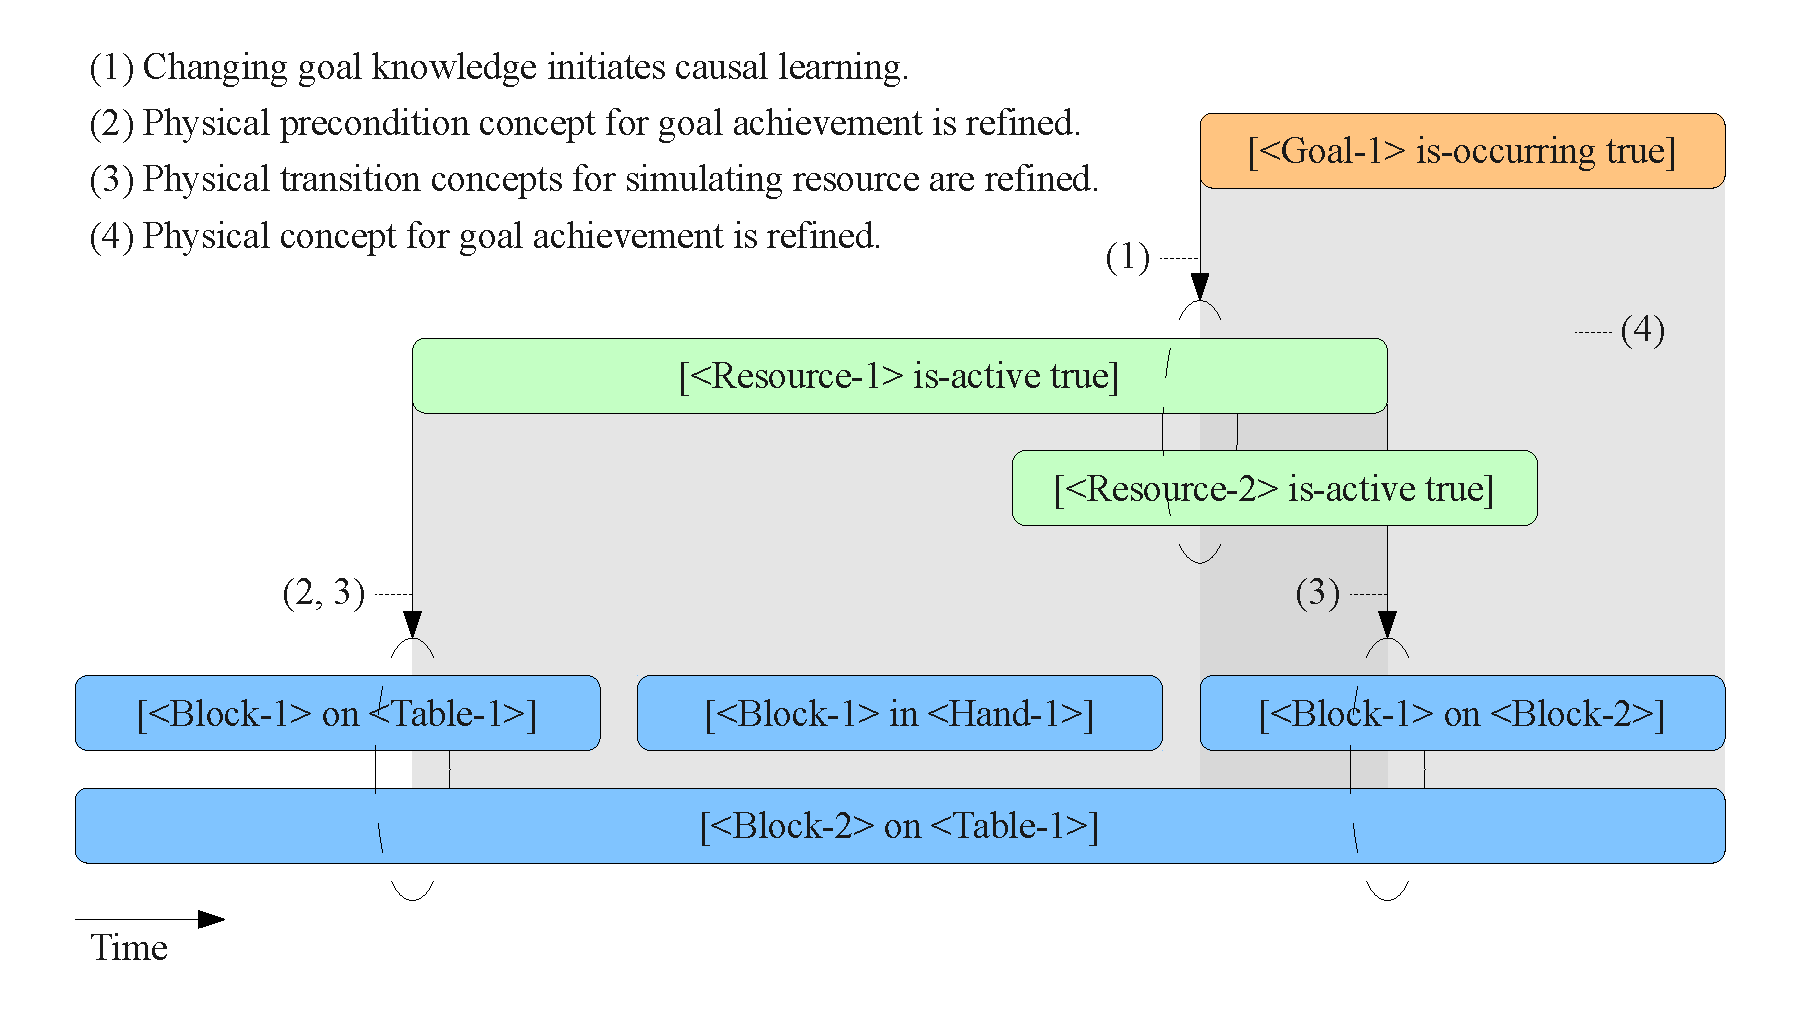
\includegraphics[width=12cm]{gfx/learning_to_plan}
  \caption[The reflective learning cycle]{The reflective learning
    cycle is a way to learn knowledge used to plan toward goals that
    maintains the causal dependency structure of the knowledge.}
  \label{fig:learning_to_plan}
\end{figure}

A system without a goal has no reason to learn the effects of its
actions.  Figure~\ref{fig:learning_to_plan} shows how the process of
learning causal models relating reflective states to physical states
is a fundamentally goal-driven process.  We show how this goal
prediction process leads to at least a four step causal chain of
knowledge learning.  It is important to point out that although the
learning process is a cycle over time, this ends up creating a causal
structure for knowledge dependency without loops---a critical property
in general to maintain for any causal representation.

These four goal-oriented cyclical learning steps build four of the
major types of knowledge that my goal-oriented inference and planning
system uses.  Let us now briefly introduce these four types of
knowledge before going into a more thorough explanation of the utility
of each.

\begin{enumerate}

\item{Goal-oriented action hypotheses: focuses and constrains the
  initial action learning search.}

\item{Action physical precondition goal occurrence hypotheses: allows
  predicting whether or not an action will accomplish the given goal
  under a given physical precondition.}

\item{Action physical precondition trans-frame hypotheses: allows for
  physically simulating the given action in a given physical state.}

\item{Physical hypotheses for predicting goal occurrence: allows for
  predicting if a given physical state implies that the goal is
  occurring.}

\end{enumerate}

Note that there are two different concepts of time that are displayed
in Figure~\ref{fig:learning_to_plan}.  It is important to not confuse
these.  The first kind of time is represented by the sequence of
change events in the knowledge structure that was reflectively traced
in order to generate the temporal event representation shown in the
figure.  This first time is represented and labelled as the horizontal
axis in the figure.  The second kind of time represented in the figure
is represented by the enumeration of the four learning steps.  This
learning process is a reflective learning process because it learns
from reflective knowledge gathered from tracing processes.

In the following four sections, we will describe the utility of each
of these four different types of learned knowledge in more detail.

\section{Goal-Oriented Action Hypotheses}
\label{sec:goal_oriented_action_hypotheses}

\begin{figure}[bth]
  \center
  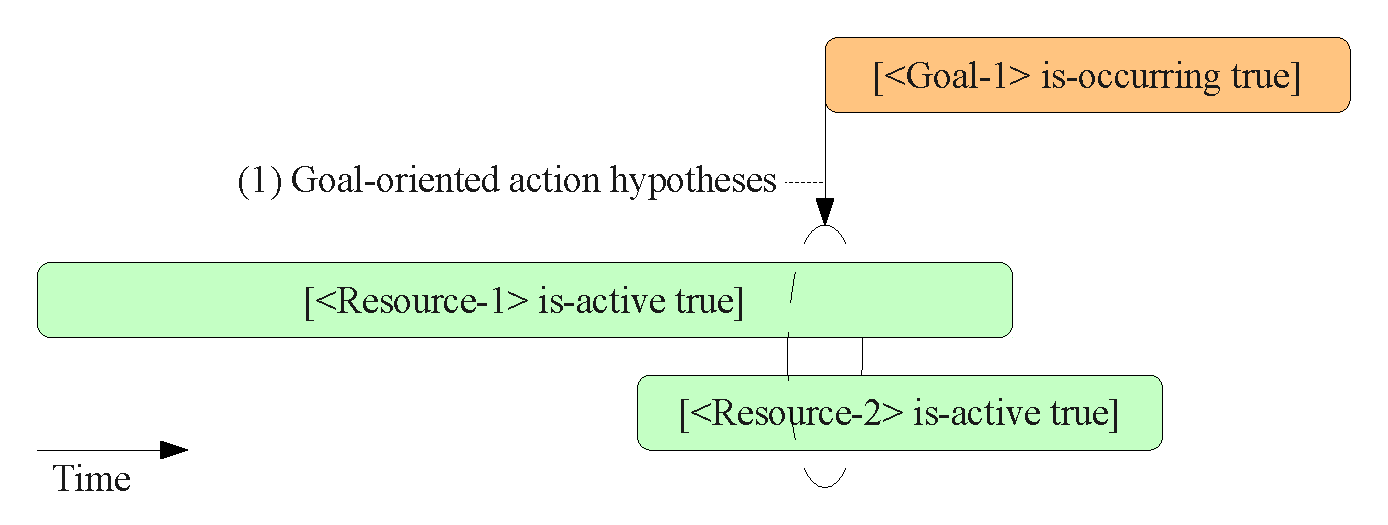
\includegraphics[width=11cm]{gfx/learning_to_plan-1-goal_oriented_action_hypotheses}
  \caption[Goal-oriented action hypothesis knowledge]{Goal-oriented action hypothesis knowledge.}
  \label{fig:goal_oriented_action_hypotheses}
\end{figure}

Figure~\ref{fig:goal_oriented_action_hypotheses} shows the first step
of the reflective learning cycle.  This first step of the learning
cycle is caused reflectively by the goal event beginning to exist.
When a goal event comes into existence, a reflective process
monitoring this goal knowledge makes a list of potential actions that
might be useful for causally predicting this goal condition in the
future.  In the figure we can see that a simple interval-point
intersection operation between the beginning point of the goal event
and any action event interval is enough to generate two actions as
initial causal hypotheses.  See
Section~\ref{sec:goal_oriented_action_hypotheses_generation_techniques}
for details on the techniques that I used for generating goal-oriented
action hypotheses in my system.


\section{Action Precondition Goal Occurrence Hypotheses}

\begin{figure}[bth]
  \center
  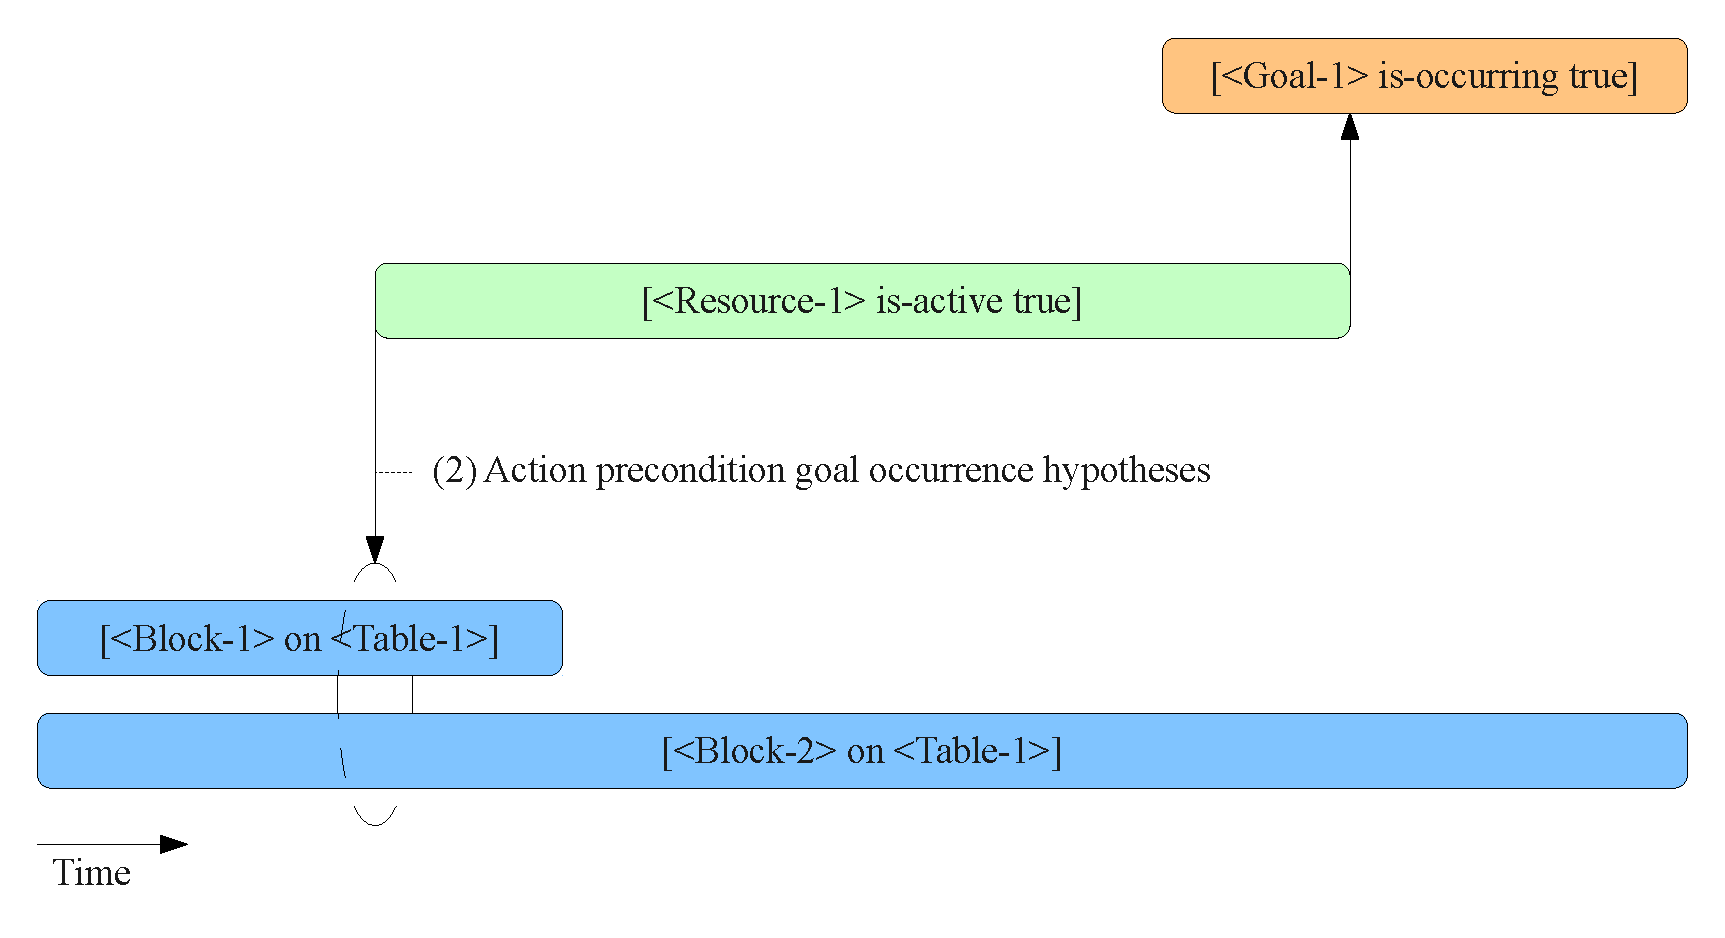
\includegraphics[width=11cm]{gfx/learning_to_plan-2-action_precondition_goal_occurrence_hypotheses}
  \caption[Action precondition goal occurrence hypotheses]{Action precondition goal occurrence hypotheses.}
  \label{fig:action_precondition_goal_occurrence_hypotheses}
\end{figure}

See Figure~\ref{fig:action_precondition_goal_occurrence_hypotheses}.


\section{Action Precondition Trans-Frame Hypotheses}

\begin{figure}[bth]
  \center
  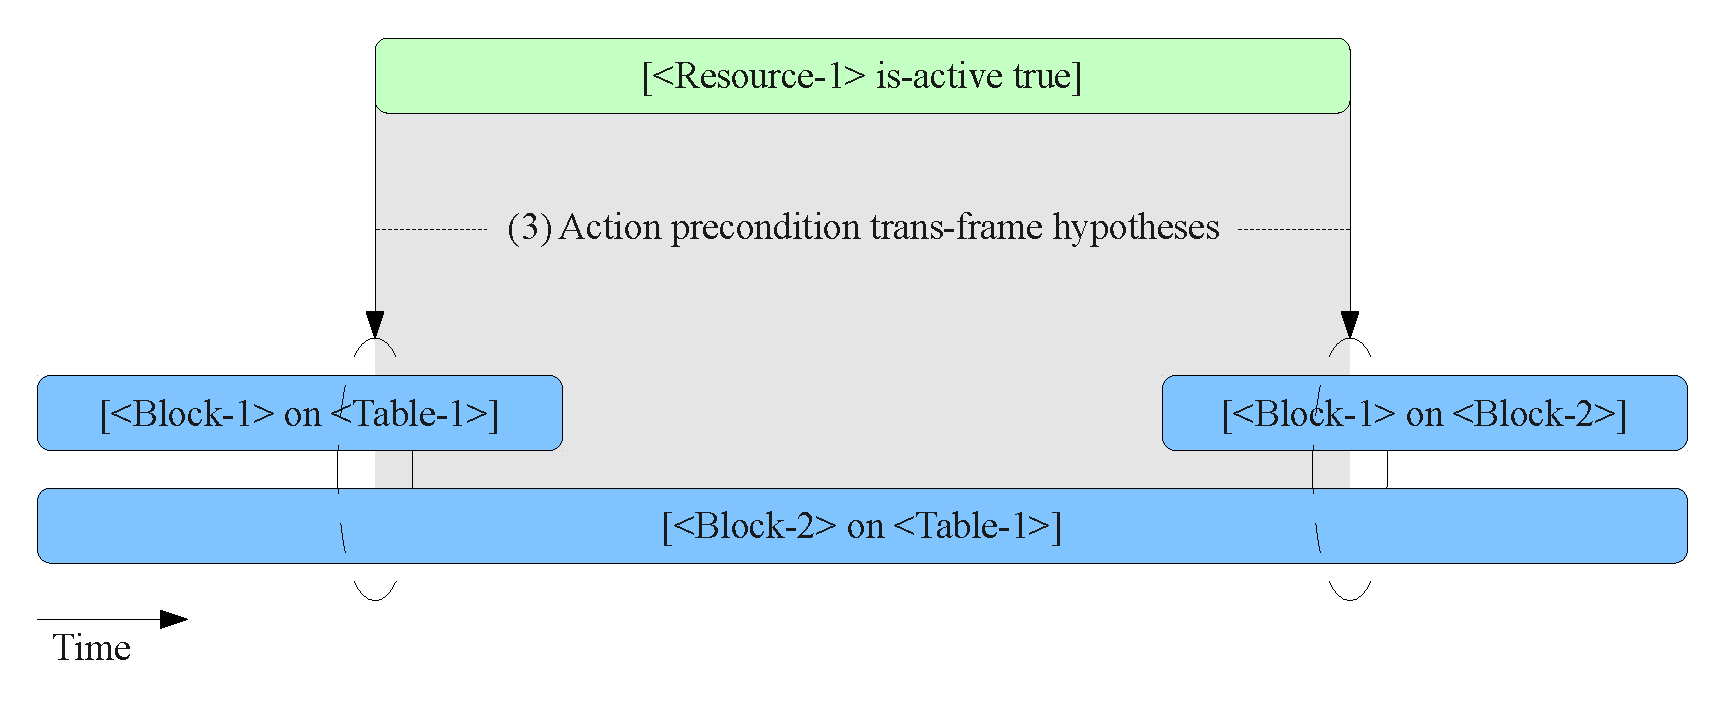
\includegraphics[width=11cm]{gfx/learning_to_plan-3-action_precondition_transframe_hypotheses}
  \caption[Action precondition trans-frame hypotheses]{Action precondition trans-frame hypotheses.}
  \label{fig:action_precondition_transframe_hypotheses}
\end{figure}

See Figure~\ref{fig:action_precondition_transframe_hypotheses}.


\section{Physical Hypotheses for Predicting Goal Occurrence}

\begin{figure}[bth]
  \center
  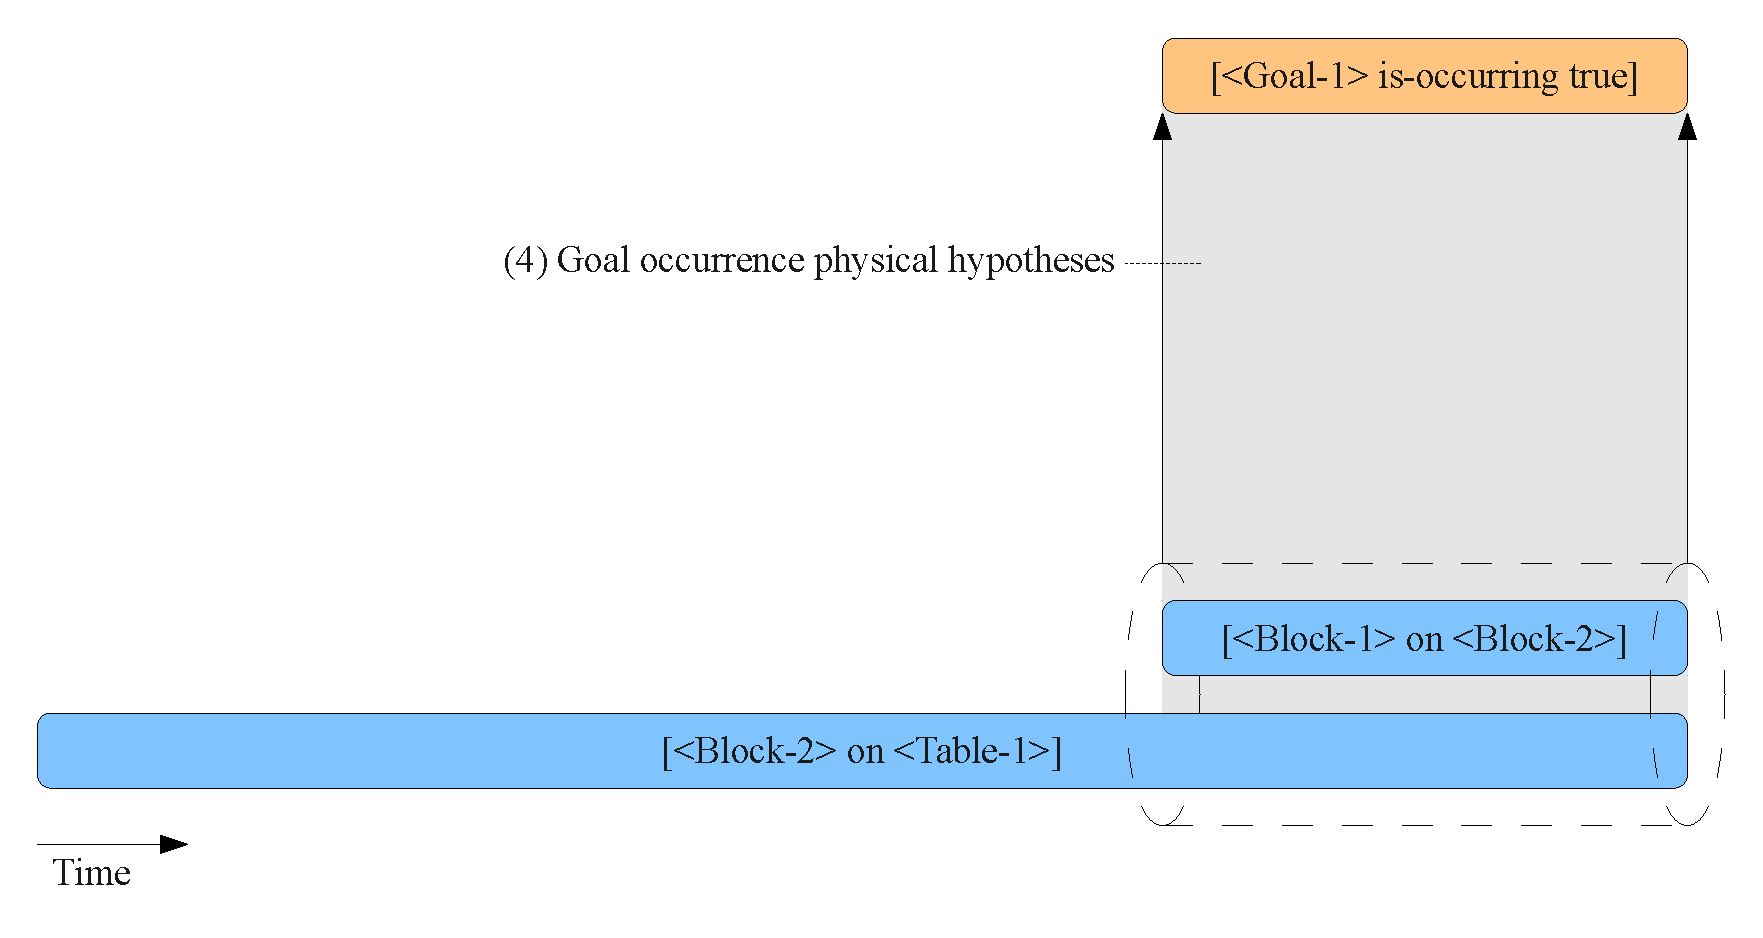
\includegraphics[width=11cm]{gfx/learning_to_plan-4-goal_occurrence_physical_hypotheses}
  \caption[Goal occurrence physical hypotheses]{Goal occurrence physical hypotheses.}
  \label{fig:goal_occurrence_physical_hypotheses}
\end{figure}

See Figure~\ref{fig:goal_occurrence_physical_hypotheses}.


\marginpar{\emph{learning goal}: focusing learning on a subset of the state space.}


\section{Learning Trans-Frames for Events}
\label{sec:learning_trans_frames_for_events}

\begin{figure}[bth]
  \center
  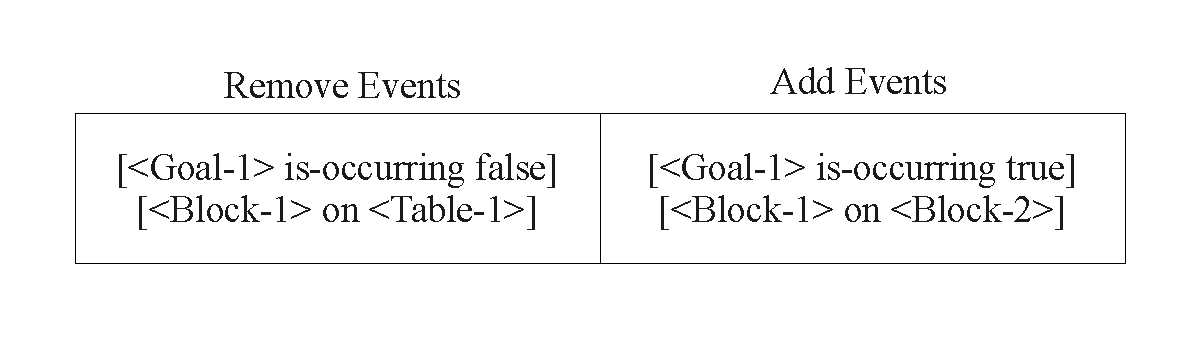
\includegraphics[width=10cm]{gfx/transframe}
  \caption[A trans-frame for an event]{A trans-frame for an event is a
    list of differences in knowledge between the beginning and ending
    of the event.}
  \label{fig:transframe}
\end{figure}

See Figure~\ref{fig:transframe}.  Also, trans-frames of trans-frames
can be thought of as a form of analogical transfer, which I further
discuss in
Section~\ref{sec:learning_analogies_as_differences_of_differences}.


\section{Partially-Ordered Plan Representation}

\begin{figure}[bth]
  \center
  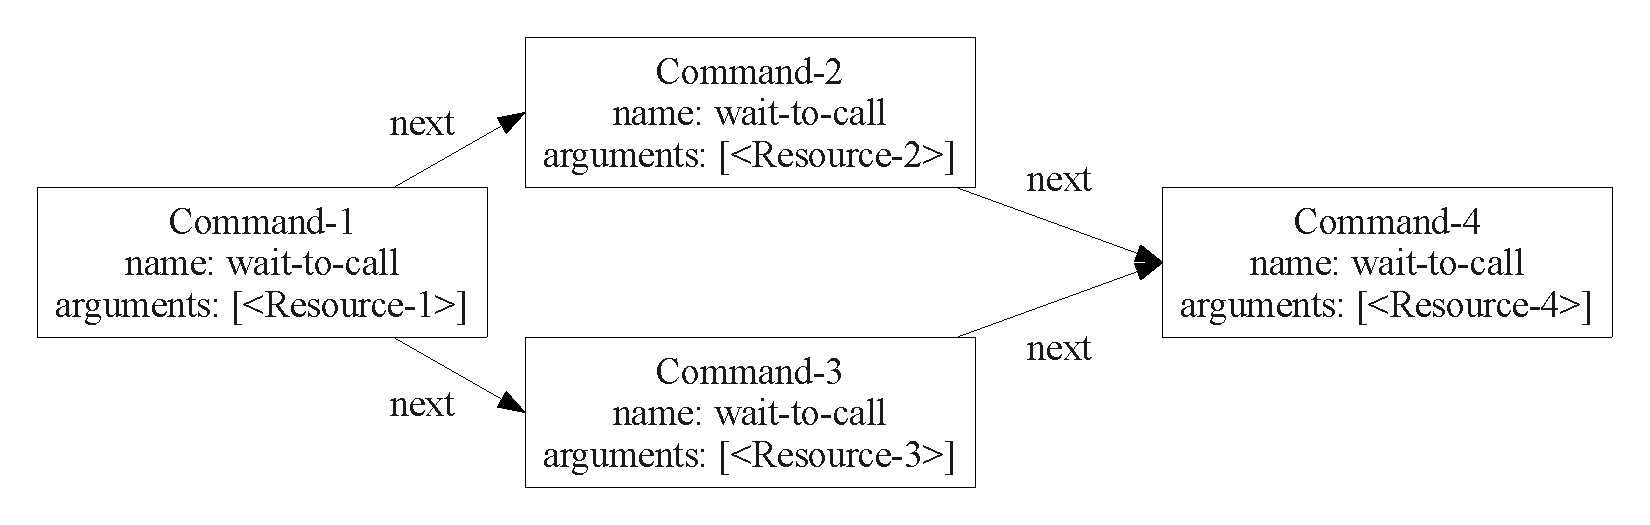
\includegraphics[width=11cm]{gfx/serial_and_parallel_plan}
  \caption[A partially-ordered plan with serial and parallel
    components]{A partially-ordered plan representation containing
    serial and parallel components.}
  \label{fig:serial_and_parallel_plan}
\end{figure}

The partially-ordered plan representation allows a partially-ordered
temporal organization for a set of commands.  A plan with a
branch-and-join control structure is shown in
Figure~\ref{fig:serial_and_parallel_plan}.


\section{Inferring the Effects of a Plan}
\label{sec:inferring_the_effects_of_a_plan}

\begin{figure}[bth]
  \center
  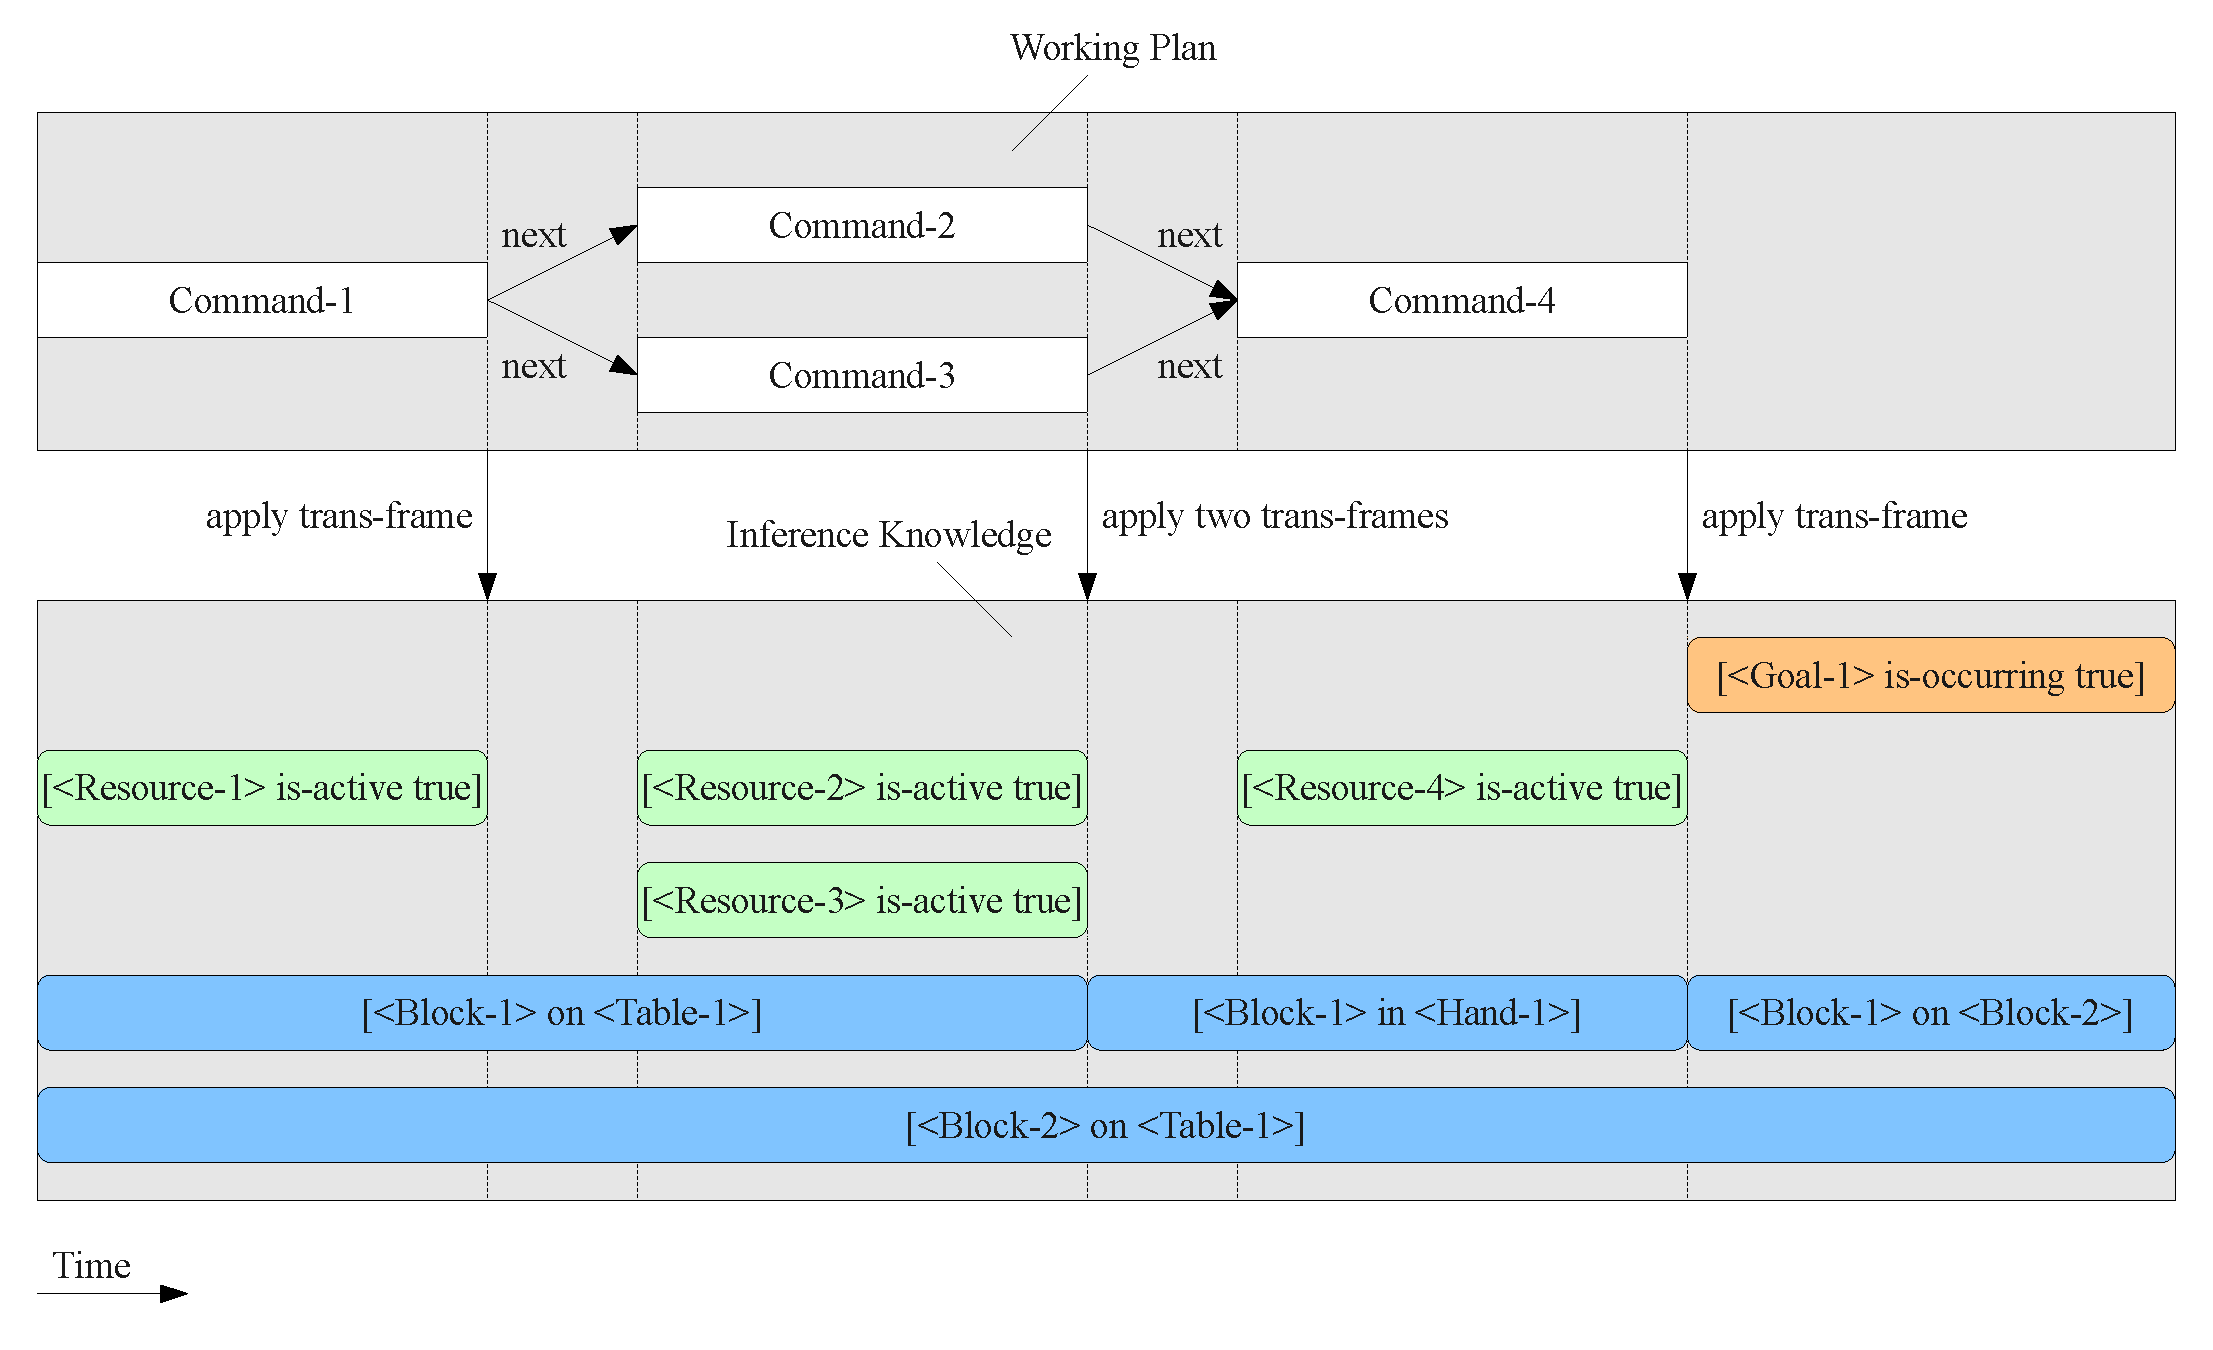
\includegraphics[width=11cm]{gfx/infer_plan_effects}
  \caption[Inferring the effects of a plan]{Inferring the effects of
    a plan.}
  \label{fig:infer_plan_effects}
\end{figure}

The planning process requires an inference algorithm to infer future
and past states based on cause-effect relationships between reflective
knowledge and physical knowledge.  Figure~\ref{fig:infer_plan_effects}
shows a possible inference for a given plan.  There are many ways to
plan and the specific planning system that I have implemented for my
experiments is discussed further in
Section~\ref{sec:details_of_inferring_the_effects_of_a_plan}.


\section{Planning Machine Operations}

\begin{figure}[bth]
  \center
  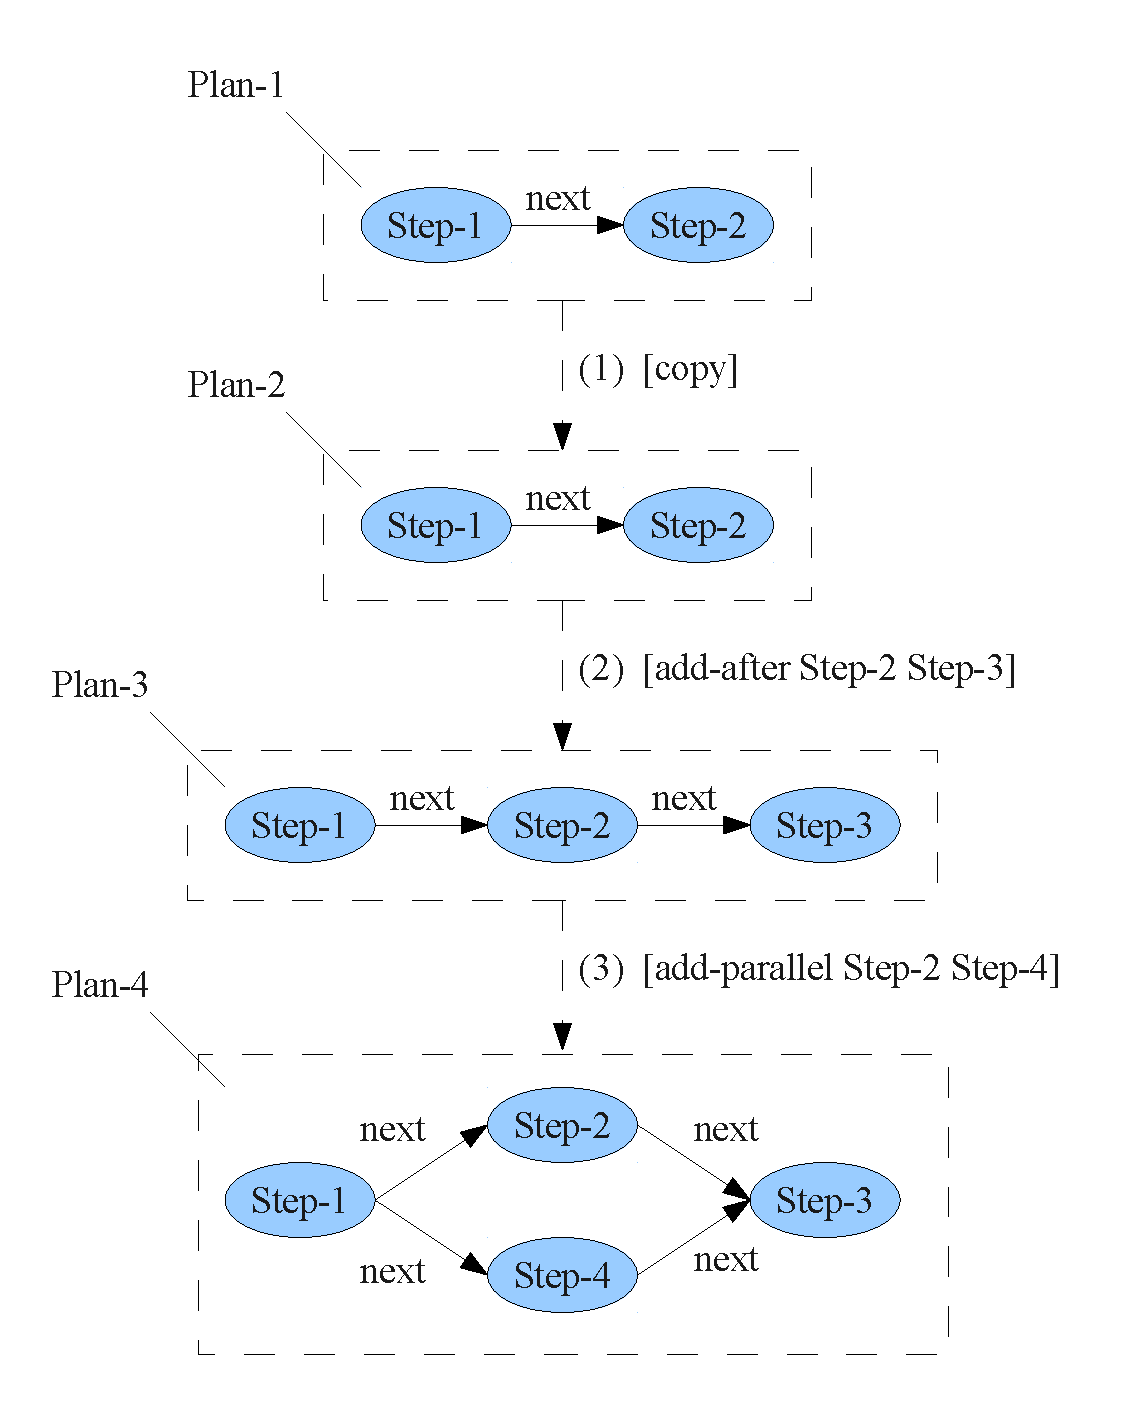
\includegraphics[height=8cm]{gfx/planning_machine_operations}
  \caption[A few planning machine operations]{A few planning machine operations.}
  \label{fig:planning_machine_operations}
\end{figure}

A few operations for manupulating partially-ordered plans are shown in
Figure~\ref{fig:planning_machine_operations}.


\section{Planning Machine Reflective Knowledge}

\begin{figure}[bth]
  \center
  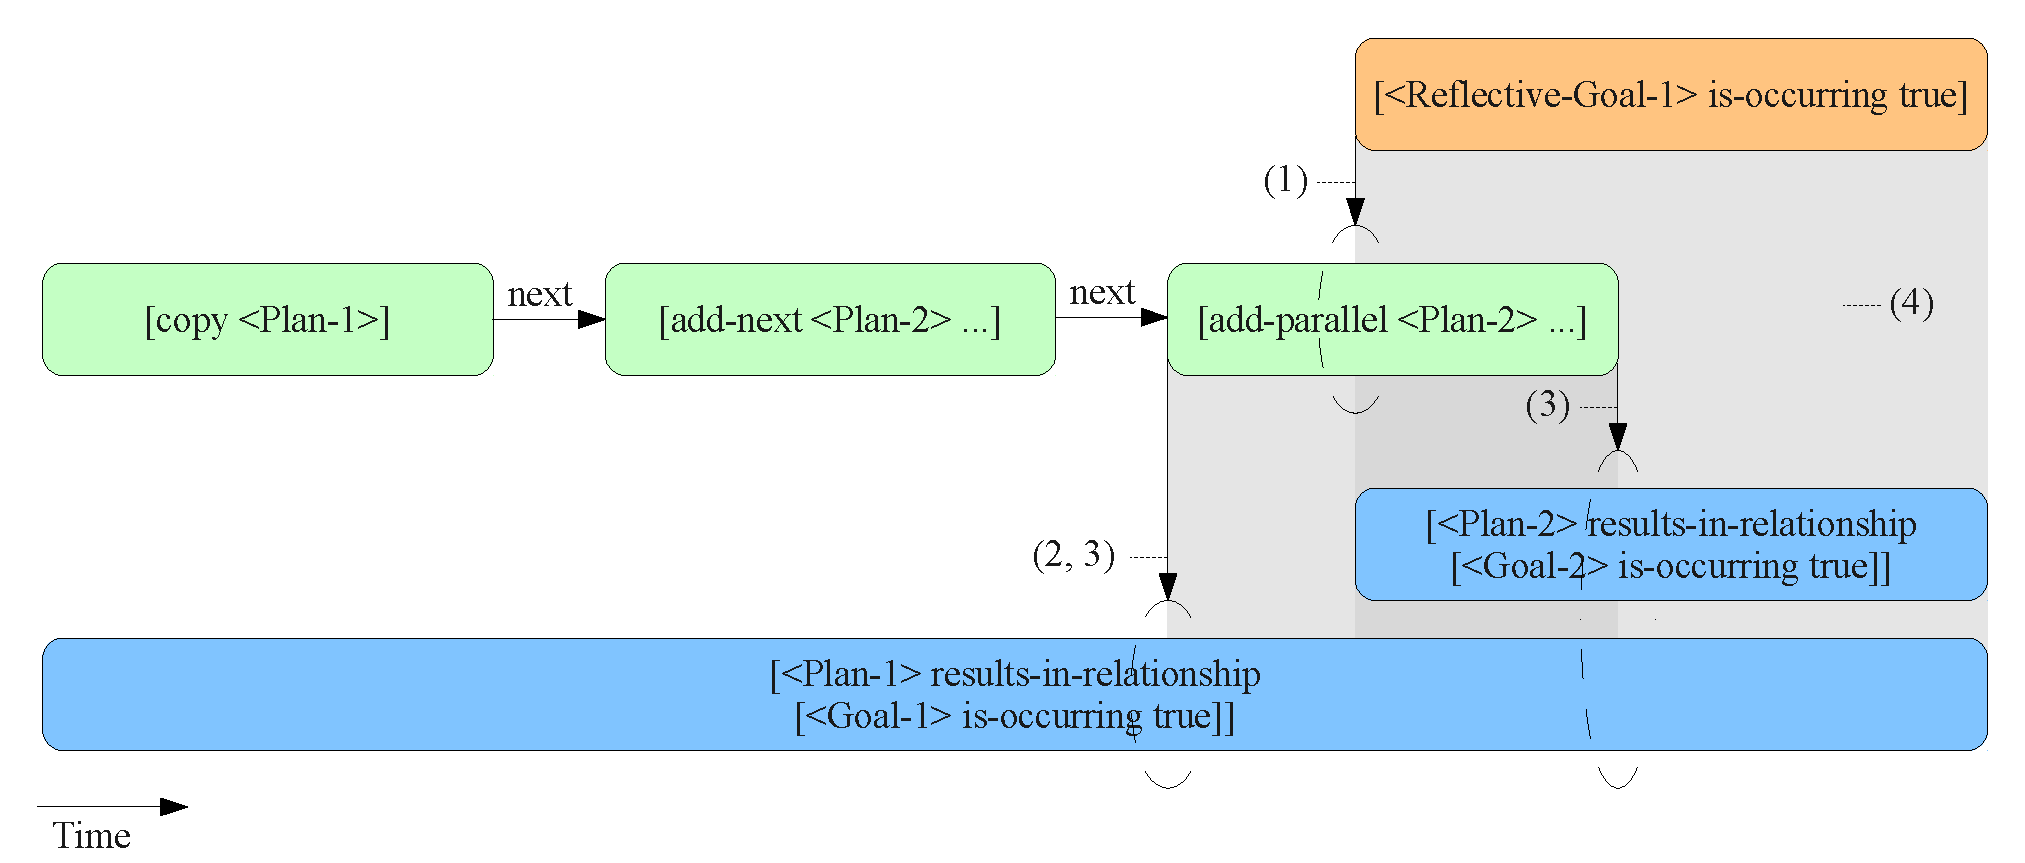
\includegraphics[width=11cm]{gfx/planning_machine_reflective_knowledge}
  \caption[Planning machine reflective knowledge]{Planning machine reflective knowledge.}
  \label{fig:planning_machine_reflective_knowledge}
\end{figure}

See Figure~\ref{fig:planning_machine_reflective_knowledge}.


%************************************************
\chapter{Problems to Solve}\label{ch:problems_to_solve}
%************************************************

\section{Build a Reflective Knowledge Substrate}

The assumption that I introduced in
Section~\ref{sec:introducing_reflection_early_in_the_process},
``Introducing Reflection Early in the Process'', requires that changes
in my knowledge representation can be traced and compiled into other
representations, such as the reflective event representations used in
learning to accomplish goals.

\subsection{Automatic Collection of Audit Trails for All Processes}

Audit trails must be collected so that after the fact the events that
any process is resposible for can be used for many types of reflective
control purposes, such as learning to plan.  Although a system that
keeps track of everything that it does would support reflection, the
audit trail recorder in a system that does not grow indefinitely in
memory consumption would have options for focusing the collection of
audit trails, while also allowing for their garbage collection when
they are no longer needed by another reflective process.

\subsection{General Parallelism and Concurrency}

\begin{figure}[bth]
  \center
  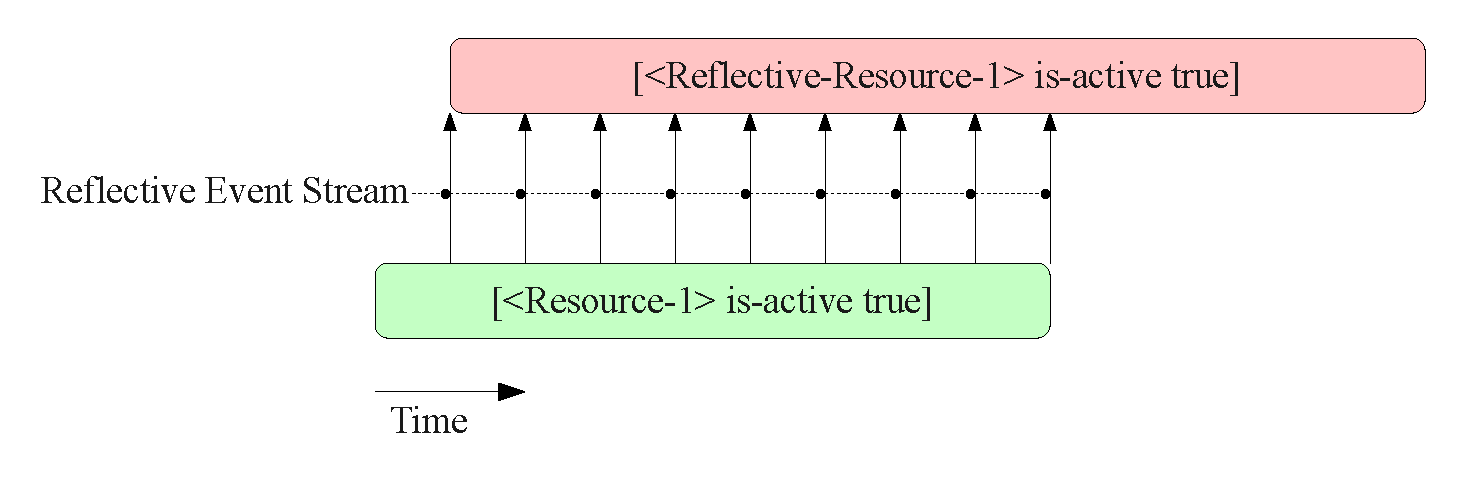
\includegraphics[width=11cm]{gfx/concurrent_parallel_reflection_efficiency}
  \caption[Concurrent parallel reflection efficiency]{Concurrent parallel reflection efficiency.}
  \label{fig:concurrent_parallel_reflection_efficiency}
\end{figure}

Because the procedurally reflective programming paradigm focuses on
event streams of changes to memory, there is an inherent ability to
express procedurally reflective algorithms in a streaming parallel
language.

Figure~\ref{fig:concurrent_parallel_reflection_efficiency} shows how a
simple process can be reflectively monitored without slowing down the
fundamental process by more than the constant time factor necessary
for generating the event stream.  Many different parallel reflective
processes can be reflectively processed concurrently without any
additional slowdown in the primary problem solving process.

\subsection{Program as Data}

The ability for a process to manipulate a program as data makes it
easier for that process or a user to read, edit, and write programs as
they are debugged.  The ability to change the functionality of a
program at run-time is a key component to creating an adaptive problem
solver.  Because of this, a programming language with a run-time
compiler is very useful for building these types of adaptive systems
that learn to debug and re-program their own subprograms.  For purely
the reason of developing problem solving learning algorithms, it is
critical that a reflective substrate has the ability to treat its own
programs as data.


\section{Layered Reflective Problem Solving}

\subsection{Analogy between Physical Goals and Planning Goals}


\section{Learning by Credit Assignment}

\subsection{Use Reflective Representations for Better Models of Learning}

\subsection{Tracing Knowledge Provenance for Credit Assignment of Success or Failure}




%*****************************************
\chapter{Theory and Alternatives}\label{ch:theory_and_alternatives}
%*****************************************

\section{Two Popular Approaches to Modelling Intelligence}

Recently, there have been two directions of research with the goal of
building a machine that explains intelligent human behavior.  The
first approach is to build a baby-machine that learns from scratch to
accomplish goals through interactions with its environment.  The
second approach is to give the machine an abundance of knowledge that
represents correct behavior.

Each of these solutions has benefits and drawbacks.  The baby-machine
approach is good for dealing with novel problems, but these problems
are necessarily simple because complex problems require a lot of
background knowledge.  The data abundance approach deals well with
complicated problems requiring a lot of background knowledge, but
fails to adapt to changing environments, for which the algorithm has
not already been trained.

\subsection{Adaptability in Complex Environments}

\begin{figure}[bth]
  \center
  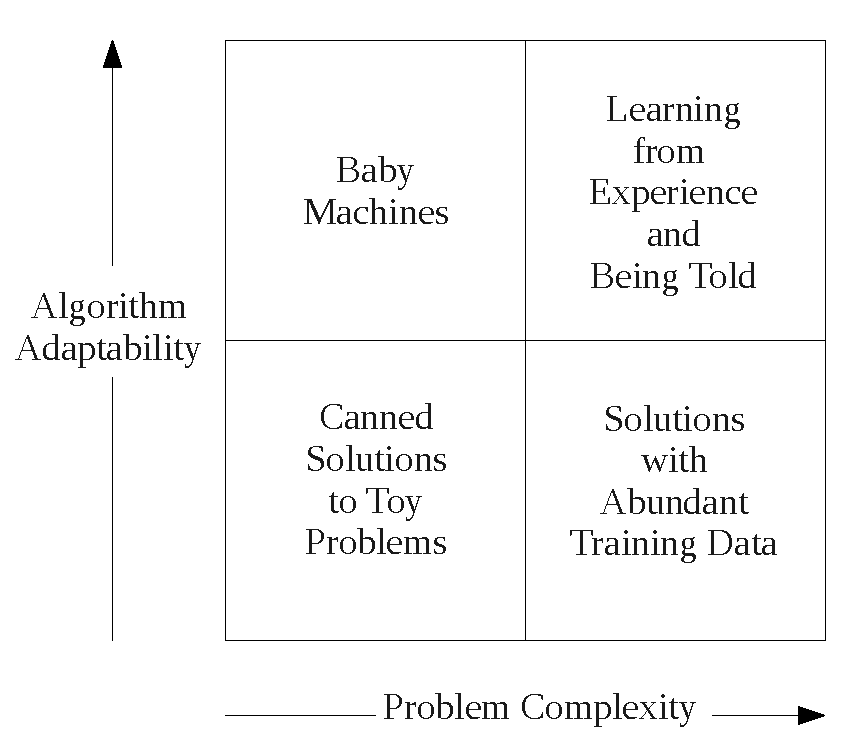
\includegraphics[height=6cm]{gfx/problem_complexity_versus_algorithm_adaptability}
  \caption[Problem complexity versus algorithm adaptability]{Problem
    complexity versus algorithm adaptability.}
  \label{fig:problem_complexity_versus_algorithm_adaptability}
\end{figure}

We would like to build intelligent machines that are able to perform
household tasks, such as cooking, cleaning, and doing the laundry, but
these tasks seem insurmountably complex, containing organically
unpredictable events.  We would like our machines to expertly handle
these extremely complicated problems, and we would also like them to
adapt to learn in unexpected or novel situations.  One popular
approach to building a machine that performs complicated tasks is to
give the machine a large training dataset that details every possible
situation that the machine may find itself within, along with the
correct action in that situation.  This is the so-called
``supervised'' learning approach.  These algorithms do not adapt to
novel situations well, and collecting these datasets is often
impossible for many problems, such as cooking and cleaning because it
is too difficult to enumerate all possible situations, in which the
machine may find itself.  Also, if the machine is cooking a meal, we
would like to be able to explain an idea for a new recipe to the
machine, or to perhaps be a partner in discovering new recipes, or we
may simply want to explain to the machine that a guest has a specific
allergy to walnuts, making that ingredient an exception for this meal
but not others.
Figure~\ref{fig:problem_complexity_versus_algorithm_adaptability}
shows how problem complexity and algorithm adaptability can be thought
of as a two-dimensional space into which different algorithmic
approaches can be used as solutions.

\subsection{The Abundant Data Approach}

There have been many approaches to modelling complex forms of
reasoning by collecting large amounts of knowledge that describes
correct or acceptable behavior in a domain.  For example, there are
examples of complex multi-agent commonsense simulation environments
collects thousands of examples of users interacting in a complicated
object-oriented social simulation \citep{orkin:2009},
\citep{orkin:2010}.  These systems have complicated domains, but these
projects do not attempt to build agents that attempt to accomplish
goals.  Instead, these systems are inference systems that simply try
to reproduce typical behavior, rather than goal-directed behavior.

There are many commonsense reasoning systems that do not interact with
simulation environments at all, but which attempt to demonstrate
commonsense reasoning by being told large amounts of knowledge.  The
Cyc project is one large such project that has been told large amounts
of logical knowledge \citep{lenat:1990}.  There is also effort
directed toward populating Cyc with knowledge automatically gathered
from the web \citep{matuszek:2005}.  The OpenMind project
\citep{singh:2002} is a project that gathers large amounts of
approximately correct commonsense knowledge from people online.  The
OpenMind knowledge has been turned into many inference systems that
can compare and generate new commonsense knowledge \citep{liu:2004a,
  liu:2004b, speer:2009}.

\subsection{The Common Sense Reasoning Problem Domain}

Common sense is the set of common reasoning abilities shared by most
people in a given social group.  Another way to say this is that
common sense is the set of reasoning abilities that one would assume
of a typical person that they meet for the first time and know nothing
about.  For example, most people have a naive theory of physics, so
you would expect someone to know that things fall when they are not
supported and liquids flow or are absorbed unless they are in a
container.  Common sense relies on a lot of knowledge that is assumed
that most everyone knows.

%TS>> what is a given social group... i share very little reasoning abiltities about user TS>>interface with my daughter or the director of CMU Siliicon Valley or my bike riding 
%TS>> friends, or my brothers,....

%TS>> not crisp enough ... a person is not defined as a person...but realtive to a 
%TS>> role we have with them,,, a mechanic talks differently to a woman or man, a professor
%TS>> or his accountant about cars 

%TS>> again, people have different theories of physics than each other 

%TS>> i have been served food in which the floating stuff  was designed to change through 
%TS>> the period of servign and eating soup  ..

%TS>> I am ready for  a fight on that , i live with a woman, a teenage girl, an autistic,
%TS>> my neighbor is a morman, the woman next door is totally rich... very diffferent 
%TS>> world views... even about how to deal with trash from a dinner. 

%TS>> I don't know what YOU mean by common sense yet,,,, define something specific
%TS>> does it cover diffferent minds or clones, what about its edges,   


Building a machine that demonstrates common sense reasoning is a
long-standing goal of the field of artificial intelligence.  One of
the difficulties in developing algorithms for dealing with a common
sense reasoning domain is that the algorithm needs a lot of background
knowledge about a given domain before it can answer even simple
questions about it.  However, this knowledge is often only true in
very specific situations and has many exceptional cases.  For example,
the knowledge that most birds can fly is generally true, but we also
know that many birds are flightless, such as penguins, ostriches, and
road runners.  Also, we have knowledge about the typical behavior of
objects; for example, we know that refrigerators keep things cold,
but we also reason efficiently about exceptional cases, such as when
the refrigerator is not plugged in, or when the power goes out.

%TS>> yes but those are examples we have seen for decades with varying 
%TS>> logical relations solving them
%TS>> show some that we haven't been able to do or places where you hold
%TS>> up where others have always been brittle 
%TS>> flexibility, integrity, hypocracy, intentionality changing belief systems...? 


\subsection{Representations for Common Sense Reasoning}

There have been many approaches to artificial intelligence that use
first-order logic as a representation for these types of knowledge and
their exceptions, but these systems become cumbersome in their
inability to express ``fuzzy'' sorts of relationships, such as when
the knowledge is applicable, for example the modifiers, ``most of the
time'', ``usually'', and ``almost never'', are difficult to express in
first-order logic.  When we have a lot of knowledge, we need ways to
keep track of in which situations this knowledge is useful.  This is a
form of ``meta-knowledge'', or knowledge about knowledge.
Meta-knowledge about first-order logic cannot be expressed in
first-order logic, so another type of representation is required for
this type of knowledge.  Therefore, we need other ways to represent
our knowledge in addition to logic.

\begin{quote}
``Nonetheless, theorem proving is in the worst case an intractable
  problem, even with no variables or unification, so no algorithm is
  going to work on the problem all the time. In this respect, theorem
  proving, for all its superficial formalism, is a lot like other
  branches of AI.  Where a theorist views a problem as solved if he
  has found an efficient algorithm or a discouraging lower bound, an
  AI researcher is often happy to find an algorithm that seems to work
  on some interesting problems, even though he doesn't really know the
  bounds of what it can do. Exploration will reveal the extent of its
  powers-each time it solves one more interesting problem something
  has been
  gained.''~---~\defcitealias{mcdermott:1987}{Drew~McDermott}\citetalias{mcdermott:1987}
\end{quote}


\section{Comparable Cognitive Architectures}

EM-ONE, Cyc, Icarus, ACT-r, Soar, and Prodigy are comparable cognitive
architectures to the one that I have built.

\subsection{The EM-ONE Cognitive Architecture}

I worked with Pushpinder Singh from 1999 to 2006 on the first version
of the Emotion Machine architecture, EM-ONE \citep{singh:2005}.
EM-ONE was an example of a reflective control system that used
commonsense stories in order to reason about social problem solving.
\cite{morgan:2009} discusses a number of things to learn from the
EM-ONE architecture that have informed my current approach.

Push and I have discussed that one weakness in the EM-ONE system is
its reliance on tracing only the declarative prolog statements, among
other necessary but untraced procedural code.  Although EM-ONE
contained a large amount of procedural knowledge, none of the effects
of this procedural knowledge could be debugged reflectively.  Toward
solving this problem, I have based my approach on a memory layer that
can trace the provenance of select memory events.

\subsection{Icarus}

Icarus is a cognitive architecture that supports a form of far
transfer learning \citep{konik:2009}.  The Icarus system allows for a
goal-directed structure mapping learning process.  These structure
mappings that are learned in this goal-directed way, can be useful
forms of analogy that enables ``far'' transfer in a cognitive system.
The Icarus work builds upon a previous model for analogical transfer
learning between symbolic relational structures \citep{gentner:1983}.

Because my knowledge representation is relational and symbolic, I see
Icarus' approaches to far transfer learning as highly compatible with
my architecture's ability to support multiple knowledge domains for a
single goal-oriented problem solving agent.  I am also interested in a
technique of using differences of differences \citep{winston:1970} as
an alternative to the structure mapping form of analogical transfer.

The Icarus system has also been applied to moral reasoning tasks in
order to build a theory of moral reasoning in humans \citep{iba:2011}.
I see similar applications of my architecture to these social
reasoning domains, but my planned approach to this domain is based on
two more layers of reflective control than I have currently
implemented \citep{morgan:2011}.

\subsection{Computational Models of Cognition about Cognition}

\cite{cox:2005} gives a good overview of the cognitive sciences that
deal with the problem of thinking about thinking, or
metacognition.

\subsection{Shades of Belief as Debugging Meta-Knowledge}

\cite{stein:1995} applies a prototype system to perform reflective
case-based reasoning over shades of beliefs in knowledge.

\section{Bounded Rationality}

There is an approach of economics and game theory that is called
bounded rationality \citep{simon:1972}.  These models deal with the
time constraints of not only acting efficiently in a domain but also
in optimizing the planning actions involved in accomplishing goals.
This approach assumes that there is an absolute numerical reward value
for accomplishing goals.  In the sense that absolute values for all of
the goals of a system are seldom known in practice, the bounded
rationality approach is limited in a general sense similar to the
simpler reinforcement learning approach.

\subsection{Feedback Control Model for Accomplishing a Single Goal}

\begin{figure}[bth]
  \center
  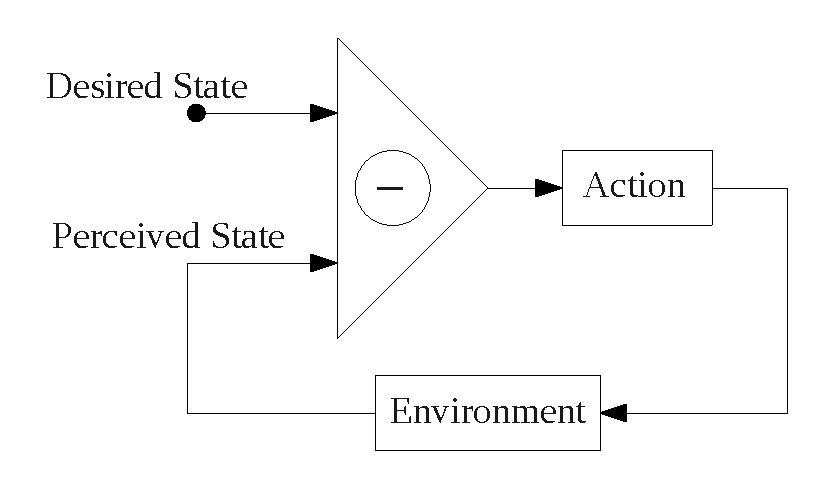
\includegraphics[width=6cm]{gfx/feedback_control}
  \caption[The feedback control model for accomplishing a single goal]{The feedback control model for accomplishing a single goal.}
  \label{fig:feedback_control}
\end{figure}

Now that we have discussed the basic model of learning from experience
what good goal states may be from rewards, let us consider the
representations for the state space of the perceptions and actions of
my model.  Control theory has given us many useful models for agents
that control continuous environments.  For example,
Figure~\ref{fig:feedback_control} shows a simple difference feedback
control circuit that is used in simple linear control systems.  The
system is given a desired state, there is a difference device that
calculates the difference between the actual perceived value from the
environment, and the control system then executes an action based on
that difference, which affects the environment.  The result in such a
negative feedback loop is that the agent's perception of the
environment is closer to the desired state.

\subsection{Means-End Analysis}

In 1959, Newell, Shaw, and Simon published a report on a means-end
analysis model that was designed to solve any symbolically represented
problem \citep{newell:1959}.  Their system was called the \ac{GPS},
and worked by being able to work with relational representations of
current and desired states.  The agent had a catalogue of differences
between states that it knew how to minimize.  The system worked by
finding the largest difference and executing the associated method for
reducing this difference.  This work has grown into the Soar model
\citep{newell:1990} for better solving symbolic planning problems, and
dealing with impasses for when the planning search runs out of
options.

\subsection{Difference-Engine Model for Accomplishing Multiple Goals}

\begin{figure}[bth]
  \center
  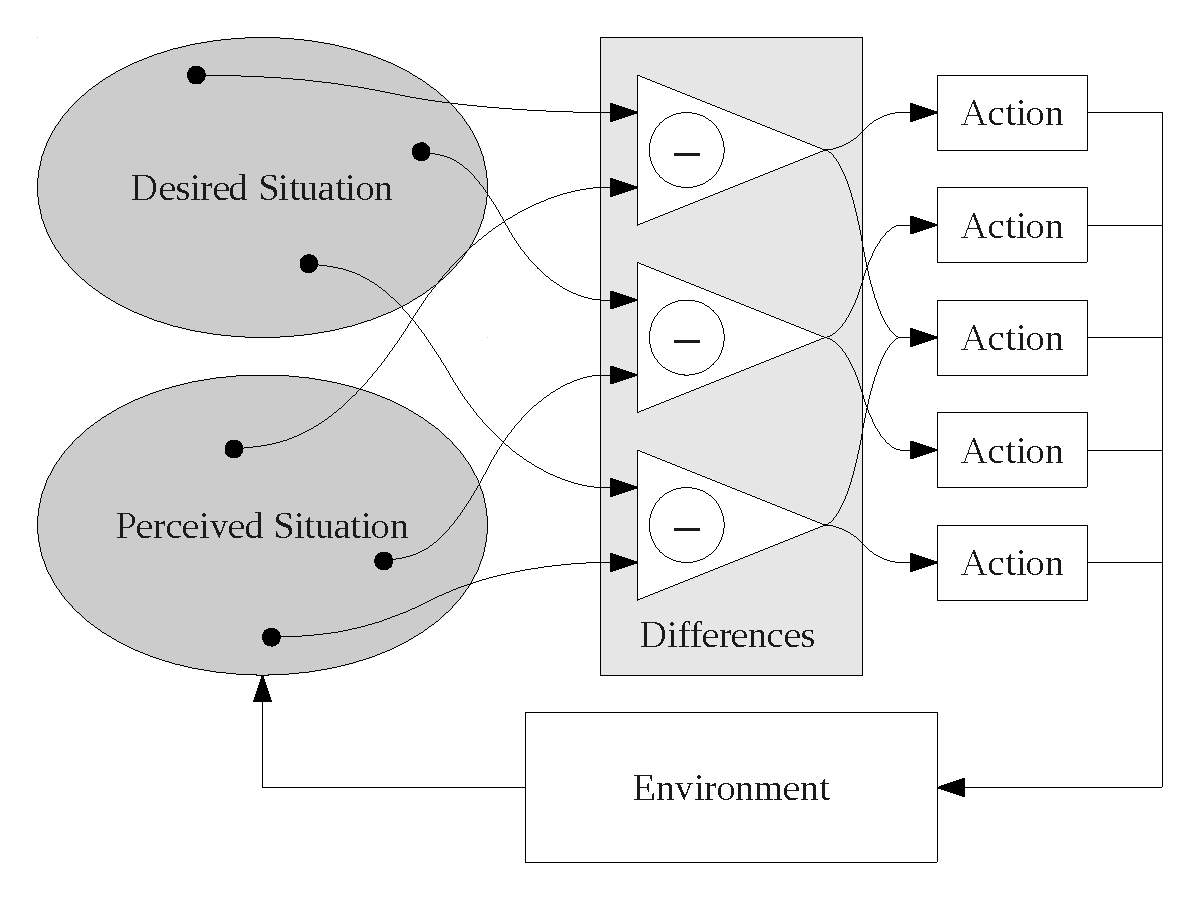
\includegraphics[height=6cm]{gfx/difference_engine_feedback_control}
  \caption[The difference engine model for accomplishing multiple goals]{The difference engine model for accomplishing multiple goals.}
  \label{fig:difference_engine_feedback_control}
\end{figure}

\citep[p.~78]{minsky:1988}



\section{Planning}

\subsection{Assuming a Correct Model of Environment}

There are many types of processes that make plans for accomplishing
goals, which make plans assuming a model of how actions theoretically
affect the environment.  These processes are called planners when they
create a representation for how actions should be performed,
potentially including temporal ordering constraints.

Planners are a specific part of a complete learning system, but the
primary function of a planner is to find a theoretical solution to a
given problem.  This theoretical solution, or plan, may be executed
and may fail or succeed, in accordance with the initial intentions for
executing the plan, the initial intentions for imagining the plan, or
any other intentions.  If the plan fails, then we may find something
to be modified in my knowledge in order to help us in avoiding this
failure next time.  The planning process is a small part of the
complete closed-loop learning algorithm that learns to plan from
experience with the environment and other agents.



If we are thinking about the temporal constraints of the problem
solving process itself, then we need to consider a reflective approach
to this control problem.

  , (1) the model of the cause-effect relationship
between actions and the world, (2) the model of cause-effect
relationships between planning actions and the creation of successful
plans.

\subsection{Declarative Programming, Logical Reasoning}


\section{Machine Learning}

One encompassing goal of the field of machine learning is to develop
systems that can accomplish goals.

For example, a Markov Decision Process contains a transfer function,
which is basically a combinational device.

Of course, this combinational device would get more complicated if I added probability.



\subsection{Why Did I Forget to Include Probability in my Theory?}



\subsection{The Reinforcement Learning Model}

\begin{figure}[bth]
  \center
  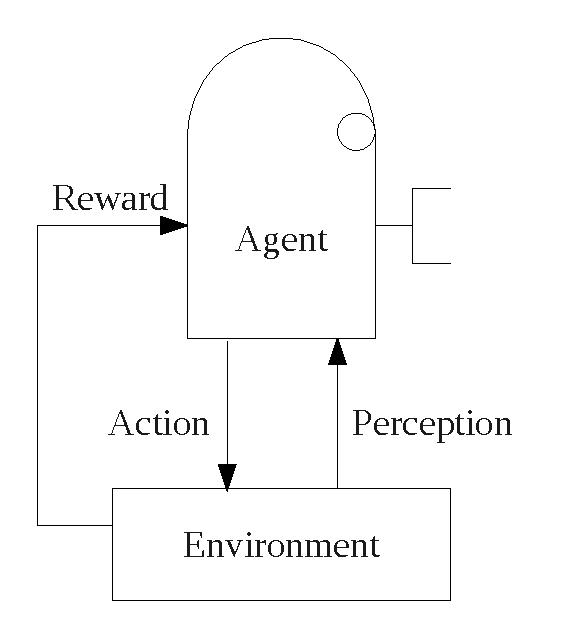
\includegraphics[height=5cm]{gfx/reinforcement_learning}
  \caption[The reinforcement learning model]{The reinforcement learning model.}
  \label{fig:reinforcement_learning}
\end{figure}

Figure~\ref{fig:reinforcement_learning} shows the basic reinforcement
learning model.  This model is an agent environment model, but there
is an extra information channel from the environment to the agent,
which communicates a numerical reward signal.  We can now say that the
agent has a learning problem.  The agent must learn what actions to
execute in order to gather the most reward.

\begin{figure}[bth]
  \center
  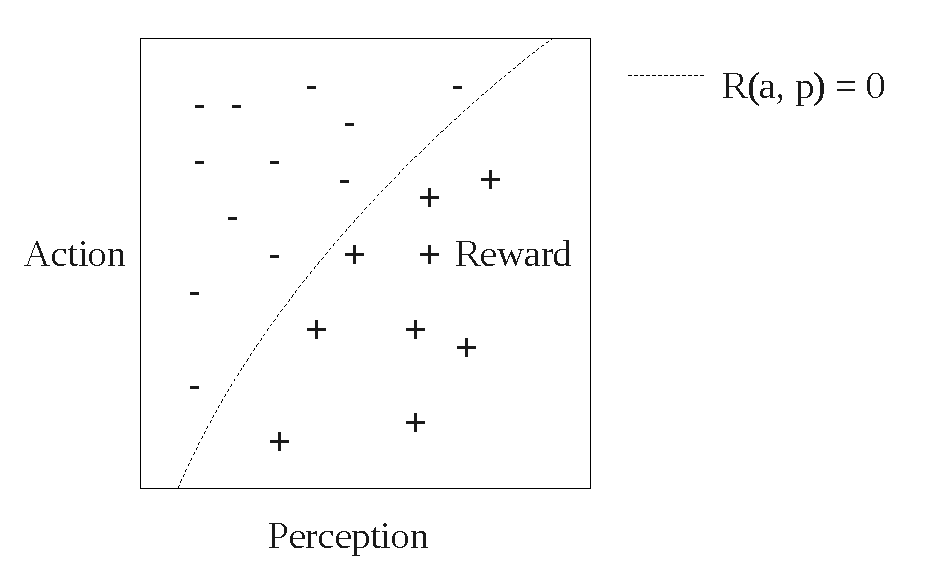
\includegraphics[height=4cm]{gfx/perception_categorization}
  \caption[Categorizing perceptions and actions based on goals]{Categorizing perceptions and actions based on goals.}
  \label{fig:perception_categorization}
\end{figure}

Once we have a basic reinforcement learning algorithm, we can approach
this learning problem as a function approximation problem.  In other
words, we can try to learn what parts of the perception and action
space have more or less reward.
Figure~\ref{fig:perception_categorization} shows a diagram of this
state space with the zero crossing of an approximation of the reward
plotted.

\subsection{Finding a Good Policy for Gathering Rewards}

Learning an approximation of what parts of a state space are good or
bad, based on reward, is not all that is needed to determine what
actions the agent should perform.  The agent wants to gather the most
rewards over time.  A simple way to formalize this problem is to learn
a policy that determines what action should be executed for every part
of the state space, based on some sort of summation of rewards over
time.  There have a been a number of ways of formalizing this
summation process as finite or infinite horizon problems
\citep{sutton:1998}.  Dynamic programming can be used for finding an
optimal or an approximately optimal policy \citep{bertsekas:1995}.

\subsection{Categorizing Perceptions and Actions based on Goals}

One problem with the reinforcement learning approach is that the only
representation of success or failure is a single number, the reward.
The basic reinforcement learning problem has been defined for finite
propositional state spaces.

A representation called \ac{RMDP} has been proposed
\citep{guestrin:2003} in order to extend reinforcement learning to
larger relational problem domains, but this method only focuses on an
object-oriented reward that does not have any global feedback about
the overall value of the situation.


\section{Philosophy}

\subsection{The Objective Modelling Assumption}

\begin{figure}[bth]
  \center
  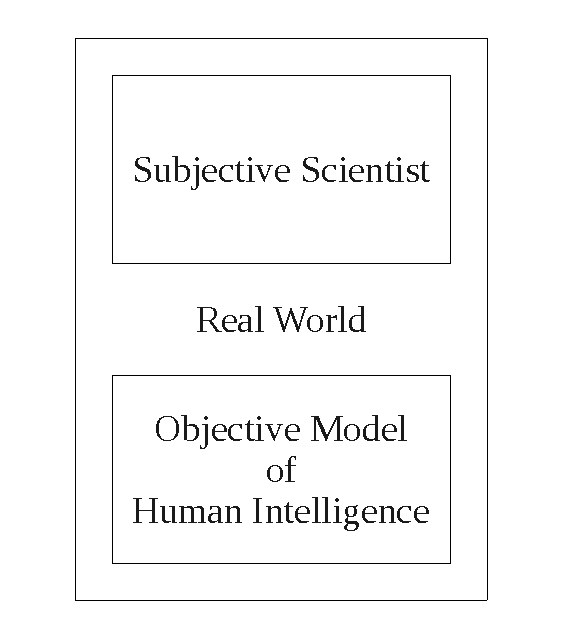
\includegraphics[width=4cm]{gfx/objective_description}
  \caption[The objective-subjective modelling assumption]{The objective-subjective modelling assumption.}
  \label{fig:objective_description}
\end{figure}

We assume that the phenomenon that we are trying to model, namely
human intelligence, is an objective process that we can describe.
This is the objective-subjective philosophical assumption that is
inherent in any objective scientific hypothesis.  We make this
assumption in order to avoid logical problems of circular causality
that occur when trying to find a non-objective description of
reflective thinking.  Figure~\ref{fig:objective_description} shows
how, given the objective assumption, the subjective scientist is part
of the real world, while she is studying an objective phenomenon.
Given the objective-subjective assumption, it would be a grave mistake
to confuse an objective model for reality itself.

\subsection{Being, Time, and the Verb-Gerund Relationship}

\subsection{The intensional stance}

\subsection{Reflective Representations}

\citep{perner:1991}


\section{Cognitive Science}


\subsection{The Development of Self-Conscious Emotions}

Between the ages of 1-3 years old, children display primary emotions,
such as joy, disappointment, and surprise.  These emotional processes
have been hypothesized to be related to the process of failing or
succeeding to accomplish a goal.  Around age 4, children begin to
display emotions that involve the self, such as guilt and shame.  It
has been hypothesized that these emotions relate to another person's
evaluation of the child's goals as good or bad.

We approach modelling this developmental process by applying Marvin
Minsky's theory of the child-imprimer relationship.  According to
Minsky's theory, at a young age, a human child becomes attached to a
person that functions as a teacher.  The imprimer could be a parent or
a caregiver or another person in the child's life, but the function of
the imprimer is to provide feedback to the child in terms of what
goals are good or bad for the child to pursue.

\subsection{Simulation Theory of Mind versus Theory Theory of Mind}


\subsection{Emotion or affect versus goal-oriented cognition}


\subsection{Embarrassment, Guilt, and Shame}



\section{Neuroscience}

\subsection{Neural Correlates of Consciousness}

\subsection{Learning by Positive and Negative Reinforcement}










\chapter{Related Background Research}
\label{other_models-chapter}

\section{The Layered ``Model-6'' Theory for Organizing Reflective Models}

Because the many fields of human cognitive modelling are so disparate
it is difficult to see them as a whole.  We are inspired by a layered
organizational scheme first presented in \cite{minsky:2006}.  The
six layers in this ``Model-6'' organizational scheme are named as
follows:

\begin{enumerate}
\item{Instinctive Reactions}
\item{Learned Reactions}
\item{Deliberative Thinking}
\item{Reflective Thinking}
\item{Self-Reflective Thinking}
\item{Self-Conscious Reflection}
\end{enumerate}

We hope that the reader will see that this is a useful way of organizing the massive amount of work that has gone into the computational modelling of abstract human thought processes since the conception of the field of artificial intelligence in 1956.
We are not claiming any biological correlations for these layers, but we are very excited by this unexplored possibility!
First, we must build such a model before any such statistical correlations could be found!
We see medical applications, such as categorizing spectrum mental disorders, as the highest-level goal in our work.

\subsection{Instinctive Reactions---Models of Insulation and Interaction}

\begin{quotation}
  \emph{We usually like to think in positive terms about how various parts of systems interact.}
  \emph{But to do that, we must first have good ideas about which aspects of a system do \emph{not} interact---since otherwise there would be too many possibilities to consider.}
  \emph{In other words, we have to understand \emph{insulations} before we can comprehend interactions.}
  \emph{To put this in a stronger form: \emph{No complicated society would actually work if it really depended on interactions among most of its parts}.}
  \emph{This is because any such system would be disabled by virtually any distortion, injury, or environmental fluctuation.}
  \emph{Nor could any such society evolve in the first place.}
\end{quotation}  

{\flushright{--- \cite{minsky:1988}}}

\subsubsection{Models of Failure in Distributed Systems}

\cite{attiya:2004} discuss algorithms for tolerating a few types of failures in distributed systems, ranging from silent crashes to arbitrary Byzantine failures, where parts of an algorithm perform in completely uncontrolled and unpredictable ways.
An algorithm for Byzantine tolerance is presented that is based upon building layers of first abstracting controllers that turn the Byzantine problem into a simpler \emph{identical Byzantine} problem.
The identical Byzantine problem is then abstracted to the simpler \emph{omission} problem, where a processor simply omits some messages from being transmitted.
The omission problem is then handled in a more abstract layer of the algorithm that when detecting an omission, crashes itself, resulting in a \emph{crash} problem.
Crash problems can be dealt in different ways for different algorithms, the simplest being the consensus algorithm.
This gives us a basic vocabulary of the most fundamental and basic distributed process problems.

\cite{bertsekas:1982} discuss a basic model for distributed dynamic programming that is organized around a distributed iterative approximation algorithm that computes a function mapping from states to values, $J(x){\in}\Re$.
His model divides the world into sets of states, $S_1 \cup S_2 \cup \cdots S_n = S$, that depend on neighboring sets of states in order to compute the approximation, $J^t$, of the optimal value function, $J^*$.
This fits with our abstract notion that commonsense knowledge in an artificial intelligence program should be organized according to what goals it is important to solve.
Having a basic optimal control theory of why this is a fundamentally sound organization principle is encouraging: perhaps organizing our knowledge by the values of goal states could also apply in the context of abstract reinforcement learning.
Note that the information theoretic organizational approaches such as the inductive logic approach used by relational reinforcement learning do not organize their knowledge according to which goal values are important for calculating which other goal values.

\subsubsection{Models of Uncontrolled Distributed Statistical Inference}
Recently, statistical propositional logic has become popular along with graph-based inference techniques for calculating both the most likely propositional state as well as the probability of any single propositional variable.
Statistical models are often represented in graphical form that can be easily distributed and computed by sparse matrix multiplication algorithms.
Given a statistical model, it is common to use the MAXENT algorithm to approximate the most likely state of such a model.
\cite{jaynes:1982} discuss when this may or may not be appropriate.
\cite{murphy:1999} discuss Pearl's ``loopy'' belief propagation algorithm which is an unreliable but efficient inference tool.
\cite{yedidia:2005} generalizes this distributed form of statistical inference to more powerful forms of hierarchical methods, explaining in the process that the forward-backward algorithm for hidden markov models, the Viterbi algorithm, Gallager's sum-product algorithm, the ``turbo-decoding'' algorithm, Pearl's ``belief propagation'' algorithm for inference on Bayesian networks, the ``Kalman filter'' for signal processing, and the ``transfer matrix'' approach in statistical mechanics are all of the same generalized form of statistical inference.

These statistical tools are the basic inference tools that claim nothing about their own applicability, and have no recourse for response for their own failures.
These statistical inference tools also know nothing about the goals which they are supposed to help solve.
In order for our algorithm to intelligently accomplish goals, we need to deliberate or plan our usage of these most basic tools.

\subsubsection{Models of Distributed Intelligence}

\cite{maes:1990} discuss learning to coordinate behavior, an argument for robust robot control using multiple ways of reasoning in a layered architecture.

\subsubsection{Models of Computational Reflection}

\cite{maes:1987} gives a great overview of ``computational reflection,'' which is basically keeping track of information about the execution of a program, so that other processes can use that information to better control the program.
Our approach to computational reflection is what they categorize as a ``frame-based'' approach, described first in \cite{minsky:1975} and first implemented in \cite{roberts:1977}.
\cite{maes:1987} describe the primary benefits of the frame-based approach as the following:

\begin{itemize}
\item{it helps the user cope with the complexity of a large system by providing documentation, history, and explanation facilities,}
\item{it keeps track of relations among representations, such as consistencies, dependencies and constraints,}
\item{it encapsulates the value of the data-item with a default-value, a form to compute it, etc.,}
\item{it guards the status and behavior of the data-item and activates procedures when specific events happen (e.g. the value becomes instantiated or changed).}
\end{itemize}

\cite{sobel:1996} discuss an introduction to reflection-oriented programming.
\cite{matsuoka:1992} discuss object-oriented concurrent reflective architectures.
\cite{oliva:1998} discuss the reflective architecture called ``Guaraná.''
\cite{watanabe:1989} discuss reflective computation in object-oriented concurrent systems.
\cite{yonezawa:1990} discuss a reflective object oriented concurrent language called ``ABCL/R.''
\cite{ancona:1998} discuss channel reification, which is a reflective model for distributed computation.
\cite{cazzola:1998} discuss evaluation of object-oriented reflective models.

\subsection{Learned Reactions---Models of Learning Reactions}

\subsubsection{Models of Planning to Perceive}

\cite{pryorcollins:1995} discuss how planning is used in perceptual processes.

\subsubsection{Models of Commonsense Reasoning}

There are many domains of quaitative commonsense reasoning, e.g. physics \cite[]{forbus:1994}, natural language \cite[]{liu:2004b}, story narratives \cite[]{williams:2005}, event planning \cite[]{smith:2006}, and psychology \cite[]{gordon:2008}.

\subsubsection{Models of Reactive Commonsense Knowledge}

There are also a few large knowledge bses of commonsense knowledge, e.g. ConceptNet \cite[]{liu:2004a}, FrameNet \cite[]{baker:1998}, Cyc \cite[]{lenat:1990}, AnalogySpace \cite[]{speer:2009}, and WordNet \cite[]{fellbaum:1998}.
Although these knowledge bases have a broad range of reasoning algorithms from linear algebraic semantic analogies in AnalogySpace to intricate microtheoretic logical deduction in Cyc, none of these knowledge bases are able to causal reflectively control the complexity of their algorithms.
Because commonsense knowledge is often represented in a declarative form, logical reasoning algorithms are often applied, but undirected logical reasoning methods often cannot handle large amounts of knowledge.
We hope that our causal reflective tools available in the Funk2 architecture will help in learning to reflectively control these explosive logical reasoning algorithms.
Another aspect that is critically important for organizing massive commonsense knowledge bases are goals; the knowledge should be indexed by types of goals.
We hope that our focus on goal-oriented learning in our reflective architecture will provide means of organizing learned knowledge in terms of the goals it is relevant for thinking about.

\subsection{Deliberative Thinking---Models of Learning to Compile Plans}

Artificial intelligence systems that use multi-step deliberation (or planning) in order to imagine hypothetical (counterfactual) sets of actions before executing these scripts (or plans) are implementing what is referred to as Layer 3 in the Emotion Machine theory of mind.

\cite{thagard:1995} discuss using a coherence theory of decision in order to perform inference to the best plan.
\cite{michalski:1995} discuss learning as goal-driven inference.

\subsubsection{Reinforcement Learning}

According to \cite{sutton:1998}, the field of reinforcement learning deals with the problem of ``learning what to do---how to map situations to actions---so as to maximize a numerical reward signal.''
Reinforcement learning is an online type of learning problem as opposed to supervised or unsupervised types of learning problems.

\cite{kaelbling:1996} gives a good overview of historical reinforcement learning.
The reinforcement learning problem is defined as

\begin{itemize}
\item{a set of states, $\mathcal{S}$,}
\item{a set of actions, $\mathcal{A}$, and}
\item{a set of scalar reinforcement signals, typically $\{0,1\}$ or $\Re$.}
\end{itemize}

It is interesting to consider how the well developed idea of ``exploration versus exploitation'' as discussed in \cite{kaelbling:1996} as a model for deciding when to sequentially meta-reason.

subsubsection{Models of Optimal Behavior}

\cite{kaelbling:1996} discuss three primary models of optimal behavior:

\begin{enumerate}
\item{the \emph{finite horizon} model in which an agent performs receding horizon control, such that total reward is $E(\sum_{t=0}^{h}{r_t})$,}
\item{the \emph{infinite discounted} model in which an agent uses future rewards discounted by a constant factor, $\gamma$, such that total reward is $E(\sum_{t=0}^{\infty}{\gamma^t r_t})$, and}
\item{the \emph{average reward} model which is the infinite limit of the finite horizon model, such that total reward is $\lim_{h{\rightarrow}\infty}{E(\frac{1}{h}\sum_{t=0}^{h}{r_t})}$.}
\end{enumerate}

Since we are dealing with modelling very large and complex systems, we see these optimality criteria as only applicable to small isolated aspects of the entire system.
Nonetheless, we hypothesize that useful approximations of optimal systems that can be derived from overlapping subsystems with constraining optimality criteria can be derived from these three basic types of optimality.
Homeostasis monitors and continual ``heartbeat'' controllers could be implemented with infinite or average optimality models, while short-term goal-oriented controllers would necessitate the complexities of the full $N$-step finite horizon model of optimality.

\subsubsection{Dynamic Programming and Optimal Control}

\cite{bertsekas:1995} describe techniques for finding optimal and approximate \emph{functional} (\emph{memoizable}) solutions to reinforcement learning control problems, using recursive formulas of flat state spaces that can be optimized very easily by using memoized functions.
While this approach does not handle abstract models of the agent's world, there are exciting options of combining a dynamic programming approach with an abstract form of reinforcement learning, such as the use of inductive logic described in \cite{dvzeroski:2001}.

\subsubsection{A Theoretical World Model}

A simple formulation of the reinforcement learning problem can be formulated in terms of Markov Decision Process (MDP) environments.
An MDP is defined as

\begin{itemize}
\item{a set of states, $\mathcal{S}$,}
\item{a set of actions, $\mathcal{A}$,}
\item{a reward function $\mathcal{R}:\mathcal{S}\times\mathcal{A}\rightarrow\Re$, and}
\item{a state transition function, $\mathcal{T}:\mathcal{S}\times\mathcal{A}\rightarrow\Pi{(\mathcal{S})}$.}
\end{itemize}

\subsubsection{Category Learning to Accomplish Goals}

Category learning in the context of goal-oriented problem-solving is an idea that is discussed by \cite{barsalou:1995}.

\subsubsection{Models of Learning by Positive or Negative Reward in the context of Relational Knowledge}

\cite{dvzeroski:2001} describe an interesting combination of inductive logic programming (ILP) \cite[]{muggleton:1992} and reinforcement learning.
The benefit of using abstract logical representations of propositional states, actions, and state values makes the basic reinforcement learning algorithm able to deal with relational state spaces, such as the blocks world toy problem and the other problem representations that we are focusing on in this PhD.
This form of learning abstractions takes a flat mental space and maps it to a hierarchical relational abstraction.

\subsection{Reflective Thinking---Models of Learning to Control Deliberation}

\subsubsection{Models of Commonsense Psychology}

Understanding human psychology in commonsense terms is an initiative described in \cite{gordon:2004}.
We see our work as building upon this development of a commonsense language for discussing the types of mental processes that humans have.
Also, \cite{gordon:2008} further develops this commonsense psychological language approach to describe the processes of self-reflection, which is even more relevant to our work.
The difference between our approach and the commonsense psychology approach is that our work simulates these mental processes in a computer, using the Funk2 causally reflective procedural programming language.
Previous approaches have represented psychological reasoning processes in a declarative logical form, but these logical forms cannot handle the large knowledge bases that are involved in general commonsense reasoning.

\cite{wilson:1977} discuss verbal reports on mental processes.
\cite{schank:1972} discuss primitive concepts underlying verbs of thought.

\subsubsection{Models of Unsticking Deliberation by Creative Analogical Thinking}

\cite{buchanan:1977} discuss creativity at the metalevel.
\cite{mueller:1990} discuss daydreamer.

A storytelling system that is called MINSTREL is discussed in \cite{turner:1994}; it is guided by creativity goals in order to develop good narratives.
The process of creative storytelling is handled very similarly to mechanical goal-oriented problem solving in this way.

\subsubsection{Models of Learning to Plan to Learn}

\cite{ram:1995a} discuss planning to learn.
\cite{desjardins:1995} discuss a decision-theoretic model for deciding what to learn next for accomplishing goals.
\cite{ram:1995b} discuss goal-driven learning in multistrategy reasoning and learning systems.
\cite{ram:1995c} discuss learning, goals, and learning goals.
\cite{cox:1999} discuss the construction of learning strategies in introspective multistrategy learning.

\subsubsection{Models of Learning by Credit Assignment through Temporal State Tracing}

\emph{Eligibility traces} are a simple reinforcement learning tool for temporal credit assignment for an agent entering positive and negative reward states.
For example, the \emph{backward} view of eligibility tracing as applied to the temporal difference, $\text{TD}(\lambda)$, learning method simply augments the basic learning algorithm with an additional eligibitity factor, $e_t(s)$, for each state.
Only non-zero values of the eligibility factor are remembered in tractible (approximate) implementations; this amounts to keeping a list of $n$ recently visited states.
In the algorithm, the current state's eligibility factor, $e_t(s_t)$, is set to $1$ and all other states are discounted by a constant eligibility discount factor, $\gamma$.
Credit assignment for rewards that are found in the world are assigned not only to the previous state, as in the basic one-step $\text{TD}(\lambda)$ algorithm but also assigned to the value functions in a discounted sense to the previous $n$ states in our eligibility trace.
We call this form of credit assignment ``Temporal State Tracing'' because it simply assigns credit to those states temporally local to the current state, i.e. there is no explicit consideration of causality involved in the assignment.

\subsubsection{Models of Learning by Credit Assignment through Causal Tracing of Failure}

We do not know of any reinforcement learning algorithms that reflectively learn how to plan through causal tracing of failures.
Our method of learning in this way is disussed in Section~\ref{causal_tracing_of_failure-section}.

\subsubsection{Models of Learning by Explaining Failures}

\cite{hammond:1990} discuss explaining and repairing plans that fail.
\cite{vanlehn:1992} discuss a model of the self-explanation effect.
\cite{ram:1995d} discuss introspective reasoning using meta-explanations for multistrategy learning.
\cite{leake:1995a} discuss goal-based explanation evaluation.
\cite{leake:1995b} discuss toward goal-driven integration of explanation and action.
\cite{dominowski:1998} discuss verbalization and problem solving.

\subsubsection{Models of Learning by Repairing Failed Plans and Inference Knowledge}

\cite{leake:1996} discuss learning to refine the case-based reasoning process through experience, introspection and expertise.
\cite{levin:2004} discuss how to span the difference between metacognitive failure and success in thinking about seeing.
\cite{cox:1996} discuss how to construct a learning strategy under reasoning failure in the terms of introspective multistrategy learning.

\subsubsection{The Difference between Metareasoning, Computational Reflection, and Causal Reflection}

\cite{hansen:2001} discuss a dynamic programming approach to monitoring and control of anytime algorithms.
\cite{cox:2007a} discuss metareasoning, monitoring, and self-explanation.
\cite{cox:2005} present a selected research review of metacognition in computation.
\cite{anderson:2007} present a review of recent research in metareasoning and metalearning.
\cite{cox:2007b} discuss perpetual self-aware cognitive agents.
\cite{cox:2008} present a manifesto on metareasoning.
\cite{davis:1980} discuss reasoning about control in terms of meta-rules.
\cite{fox:2001} discuss introspective reasoning for index refinement in case-based reasoning.
\cite{maes:1988} discuss issues in computational reflection.
\cite{minsky:1968} discuss matter, mind, and models.
\cite{newell:1982} discuss the knowledge level.

\subsubsection{Empirical Models of Reflective Thought}


\cite{baumeister:2007} discuss How emotion shapes behavior: Feedback, anticipation, and reflection, rather than direct causation.
\cite{vince:2002} discuss Organizing reflection.
\cite{mirvis:2008} discuss Executive Development Through Consciousness-Raising Experiences.
\cite{michalsky:2007} discuss Developing Students' Metacognitive Awareness in Asynchronous Learning Networks in Comparison to Face-to-Face Discussion Groups.
\cite{bivona:2008} discuss Executive function and metacognitive self-awareness after Severe Traumatic Brain Injury.
\cite{irannejad:2001} discuss The brain-mind cycle of reflection.
\cite{phillips:2005} discuss Self-awareness and the emotional consequences of self-discrepancies.
\cite{silvia:2006} discuss Emotion concepts and self-focused attention: Exploring parallel effects of emotional states and emotional knowledge.
\cite{lynn:2008} discuss The eq interview: finding employees with high emotional intelligence.


\subsection{Self-Reflective Thinking---Models of Control using Self and Other Models}

\cite{anderson:2005} discuss the metacognitive loop and the problem of brittleness in terms of logic, self-awareness and self-improvement.
\cite{schubert:2005} discuss some knowledge representation and reasoning requirements for self-awareness.

\subsubsection{Models Involving Multiple Agents}

Models of multiple intelligent agents that work together to solve problems have become popular in the field of machine learning called ``multi-agent reinforcement learning.''
Many popular surveys of the field exist \cite[]{wei:1995} \cite[]{sen:1999} \cite[]{stone:2000} \cite[]{shoham:2004} \cite[]{yang:2004} \cite[]{panait:2005}.

\cite{boutilier:1996} discuss a specific type of $n$-person cooperative game theory, in which agents share common goals, or in other words, a joint value function.
\cite{rapoport:2001} discuss $n$-person game theory in more detail.

\cite{bowling:2000} describe an analysis of stochastic game theory for multiagent reinforcement learning.
\cite{claus:1998} describe the dynamics of reinforcement learning in cooperative multiagent systems.
\cite{crites:1998} describe elevator group control using multiple reinforcement learning agents.
\cite{ghavamzadeh:2006} describe hierarchical multi-agent reinforcement learning.
\cite{guestrin:2002} describe coordinated reinforcement learning.
\cite{hu:1998} describe a theoretical framework and an algorithm for multiagent reinforcement learning.
\cite{kapetanakis:2002} describe reinforcement learning of coordination in cooperative multi-agent systems.
\cite{mataric:1997a} describe reinforcement learning in the multi-robot domain.
\cite{park:2001} describe modular $Q$-learning based multi-agent cooperation for robot soccer.
\cite{sandholm:1996} describe multiagent reinforcement learning in the iterated prisoner's dilemma.
\cite{tan:1997} describe independent versus cooperative agents in multi-agent reinforcement learning.
\cite{wang:2003} describe reinforcement learning to play an optimal Nash equilibrium in team Markov games.

\subsubsection{Multiagent Reinforcement Learning with Layered Models}
\cite{stone:1997} describe layered Learning in multiagent Systems.

\subsubsection{Multiagent Reinforcement Learning with Communication}

\cite{drogoul:1994} describe an application to social differentiation in ant colonies using a multi-agent simulation as a tool for modeling societies.
\cite{fischer:2004} describe hierarchical reinforcement learning in communication-mediated multiagent coordination.
\cite{price:1999} describe implicit imitation in multiagent reinforcement learning.
\cite{sen:1998} describe individual learning of coordination knowledge.

\subsubsection{Multiagent Reinforcement Learning with Self- and Other- Models}

\cite{mataric:1997b} describe learning social behavior.
\cite{nagayuki:2000} describe an approach based on the otheragent's internal model in multi-agent reinforcement learning.
\cite{noble:2004} describe social learning in a multi-agent system.
\cite{nowe:2001} describe social agents playing a periodical policy.

\subsubsection{Models of Parent and Child Social Functions}
\cite{castelfranchi:2001} describe the challenges for computational social science and multi-agent learning in a theory of social functions.


\subsubsection{Empirical Models of Inferring Person Traits}

\cite{asch:2005} discuss how impressions of personalities are formed.
They break personality down into $18$ two-part models, or dimensions (not necessarily independent).
These 18 dimensions are listed in the following table for reference:

\begin{tabular}{rll}
  1.         & generous           & ungenerous \\
  2.         & wise               & shrewd \\
  3.         & happy              & unhappy \\
  4.         & good-natured       & irritable \\
  5.         & humorous           & humorless \\
  6.         & sociable           & unsociable \\
  7.         & popular            & unpopular \\
  8.         & reliable           & unreliable \\
  9.         & important          & insignificant \\
  10.        & humane             & ruthless \\
  11.        & good-looking       & unattractive \\
  12.        & persistent         & unstable \\
  13.        & serious            & frivolous \\
  14.        & restrained         & talkative \\
  15.        & altruistic         & self-centered \\
  16.        & imaginative        & hard-headed \\
  17.        & strong             & weak \\
  18.        & honest             & dishonest \\
  \emph{19.} & \emph{warm}        & \emph{cold} \\
  \emph{20.} & \emph{intelligent} & ~ \\
  \emph{21.} & \emph{envious}     & ~
\end{tabular}	      

\cite{winter:2005} discuss the difference between \emph{dispositional} inferences and \emph{situational} inferences.
A dispositional statement is a statement about the relationship between person models, such as ``kind person'' or ``she helped the man'', whereas a situational statement is a statement that does not refer to such a model of a social relationship between person models, such as ``she dropped the groceries''.
Here is the list of 18 dispositional properties that they discovered in their research interviewing college students for word associations:

\begin{tabular}{rl}
  1. & generous          \\
  2. & rude              \\
  3. & good worker       \\
  4. & helpful           \\
  5. & ill-mannered      \\
  6. & thrifty           \\
  7. & talented          \\
  8. & bigot             \\
  9. & friendly          \\
  10. & concerned citizen \\
  11. & absent-minded     \\
  12. & kindhearted       \\
  13. & cheap             \\
  14. & clever            \\
  15. & inconsiderate     \\
  16. & willpower         \\
  17. & considerate       \\
  18. & clumsy
\end{tabular}

\subsubsection{Empirical Models of Self and Other Social Models}

This section discusses much research that often uses words that we often do not see used precisely.
For example, the phrase ``self-awareness'' is often used to describe a sort of mental process that monitors another mental process.
In this document, we try to be consistent by using the word ``self'' to only refer to models of self versus other in terms of agents thinking about personalities or properties of agents.
Other common uses of the terms ``self-awareness'' and ``self-consciousness'' are often less clear and refer to any kind of reflective process perceiving the execution of another process within the mind.
There are many forms of reflective thought, and we choose to use the term ``self-reflection'' to refer to those reflective processes that deal with self and other personality models of inter-agent relationships.

\cite{goverover2007tis} discuss treatment to improve self-awareness in persons with acquired brain injury.
\cite{baumeister1993etl} discuss when ego threats lead to self-regulation failure: negative consequences of high self-esteem.
\cite{gilbert2005ocb} discuss perceptions of people.
\cite{ross2005bispc} discuss social roles, social control, and biases in social-perception processes.
\cite{hobson2006sad} discuss self-awareness in developmental perspective.
\cite{hutchinson2007saa} discuss relationships among adaption-innovation, self-monitoring, and self-consciousness.
\cite{keenan2007crr} discuss the selective causal role of the right hemisphere in self-awareness.
\cite{morin2004lca} discuss a comparison and integration of various views of the levels of consciousness and self-awareness.
\cite{silverman2008osr} discuss self-reflection.
\cite{smith2007sap} discuss self-awareness, perspective-taking, and self-face recognition.
\cite{soeiro2008svtsf} discuss state versus trait self-focus: comparing self-awareness to self-consciousness.
\cite{uhlmann2008vsc} discuss varieties of social cognition.
\cite{burns1998scc} discuss individual selves, self-awareness, and reflectivity in the social construction of consciousness.
\cite{duval2002sap} discuss self-awareness, probability of improvement, and the self-serving bias.
\cite{focquaert2008ecn} discuss an evolutionary cognitive neuroscience perspective on human self-awareness and theory of mind.
\cite{whitehead2001sma} discuss social mirrors and shared experiential worlds.


\subsubsection{Empirical Models of Person Groups}

\cite{menon2005cacoa} discuss the attribution to individual versus group dispositions in culture and the construal of agency.

\subsection{Self-Conscious Reflection---Models of Learning by Imprimer Reflection on Self and Other Models}

\subsubsection{Empirical Models of Imprimers}

\cite{hinton2008rlsa} discuss The Role of Leader Self-Awareness in Building Trust and Improving Student Learning.
\cite{taylor2007cfetla} discuss A Conceptual Framework and Empirical Test for Leader Attunement: Toward a Theory of Leader Self-Awareness.
\cite{hare1993wc} describe Without Conscience: The Disturbing World of the Psychopaths Among Us.

\subsubsection{Moral Decisions and Values}

\cite{harsanyi1980rur} discuss rule utilitarianism, rights, obligations and the theory of rational behavior.
\cite{duval1999osa} discuss how changing self or changing standards of correctness also changes objective self-awareness and causal attributions for self-standard discrepancies.


\section{Natural Language in Problem-Solving}

\cite{bobrow1968nlicpss} discuss Natural Language Input for a Computer Problem-Solving System



\section{Models of Story and Language Understanding}


\cite{rammoorman1999toru} discuss understanding language understanding in terms of Toward a Theory of Reading and Understandin.
\cite{rapaport1999caf} discuss understanding language understanding in terms of Cognition and Fiction.
\cite{mahesh1999spiu} discuss understanding language understanding in terms of Sentence Processing in Understanding: Interaction and Integration of Knowledge Sources.
\cite{domeshek1999ctccn} discuss understanding language understanding in terms of Capturing the Contents of Complex Narratives.
\cite{ram1999toqqa} discuss understanding language understanding in terms of A Theory of Questions and Question Asking.
\cite{peterson1999sct} discuss understanding language understanding in terms of Semantic Correspondence Theory.
\cite{moorman1999crunc} discuss understanding language understanding in terms of Creativity in Reading: Understanding Novel Concepts.
\cite{coxram1999sual} discuss understanding language understanding in terms of On the Intersection of Story Understanding and Learning.
\cite{gerrig1999tpanw} discuss understanding language understanding in terms of Text Processing and Narrative Worlds.

\section{Evaluating Models of Complex Learning}


\subsection{Evaluating Models of Learning Skill Knowledge}
\cite{anderson1993alps} describe a model of complex learning about Acquisition of LISP Programming Skill.
\cite{ohlsson1993ibkpacs} describe a model of complex learning about The Interaction Between Knowledge and Practice in the Acquisition of Cognitive Skills.

\subsection{Evaluating Models of Learning by Self-Explanation}
\cite{vanlehn1993lbeeo} describe a model of complex learning about Learning by Explaining Examples to Oneself: A Computational Model.
\cite{kieras1993lsepe} describe a model of complex learning about Learning Schemas from Explanations in Practical Electronics.
\cite{rosenbloom1993bpebl} describe a model of complex learning about Bias in Planning and Explanation-Based Learning.

\subsection{Evaluating Models of Learning Declarative Relational Knowledge}
\cite{huffman1993cidt} describe a model of complex learning about Correcting Imperfect Domain Theories: A Knowledge-Level Analysis.
\cite{hammond1993csacbp} describe a model of complex learning about A Cognitive Science Approach to Case-Based Planning.
\cite{wilensky1993kanlp} describe a model of complex learning about Knowledge Acquisition and Natural Language Processing.

\subsection{Visual Programming Languages for Psycological Study of Complex Models}

\cite{cooper2002mhl} and \cite{cooper1998cvd} discuss how to model high-level cognitive processes in an empirical and scientific way.
Much of their work is presented in terms of their COGENT cognitive architecture that includes a visual programming language for cognitive scientists to quickly build and evaluate varieties of complex hypotheses.

\cite{cooper1995too} discuss an object-oriented language for cognitive modeling
\cite{cooper1996smc} discuss A systematic methodology for cognitive modelling
\cite{cooper1998ced} discuss COGENT: An environment for the development of cognitive models
\cite{councill2003esa} discuss Explaining Soar: Analysis of existing tools and user information requirements
\cite{mulholland1998hfc} discuss Hank: A friendly cognitive modelling language for psychology students
\cite{mulholland1999pph} discuss Programming with a purpose: Hank, gardening and schema theory
\cite{mulholland2000lbv} discuss Learning by building: A visual modelling language for psychology students
\cite{yule2001ttc} discuss Towards a technology for computational experimentation

\section{Models of the Large-scale Integration of Multiple Models of Cognition}

\cite{langley2008car} gives a good overview of the current state of the field of cognitive architectural design in terms of what exists and what needs to still be designed and built.
Among the features that are not much explored are the types reflective processes that control deliberative processes, which \cite{sloman2001vaa} refers to as meta-management.
We see building layers of these reflective management processes in the top three layers of the Emotion Machine theory as our basic inspiration for higher orders of reflective control beyond meta-management.

\subsection{The EM-ONE Model}

\cite{singh2005one} describe the first cognitive architecture based on the Emotion Machine theory of mind, developed in \cite{minsky2006em}.
This architecture includes the ability to control reasoning using a relational list commonsense narrative representation.
In terms of types of representations, the Emotion Machine theory proposes that self models exist in the self-reflective layer and imprimer models exist in the self-conscious layer.
Our purpose is to elaborate on this example model in a much larger and more powerful causally reflective programming language.
Our Funk2 architecture is based on procedural forms of run-time reflection that is built into the underlying programming language, whereas the previous work was based on declarative forms that used an assortment of programming languages, including Lisp and Prolog.

\subsection{The Icarus Model}

\cite{langley2005aap} describe an architecture that uses meta-knowledge of knowledge.
They refer to skill planning as planning toward long-term goals in the abstract meta-knowledge plan space.
They refer to short-term planning as planning over instances of the skill plans.
We see our approach as complimentary to this plan abstraction approach because we are focused on adaptive learning due to failures of conflicting plans, so we expect our approach to be adaptable to this form of meta-planning as well.

\subsection{The ACT-r Model}

\cite{anderson2004itm} describe a model that is inspiring to us because it is the largest cognitive architecture that is actively being correlated to human neurological and psychological data.
We see our work as heading in this direction, but first we must complete a working model of our theory so that such similar scientific work may proceed in terms of understanding reflective, self-reflective, and self-conscious thought processes!

\subsection{The SOAR Model}

\cite{laird1987sag} describe SOAR: An architecture for general intelligence.
\cite{marinier2009cuc} describe a recent use of SOAR: A computational unification of cognitive behavior and emotion.

\subsection{The PolyScheme Model}

\cite{cassimatis2004icp} and \cite{cassimatis2006csa} describe a cognitive architecture that combines multiple representations and reasoning methods for implementing human level intelligence.
We see the problem of having multiple representations and concurrent reasoning processes as exactly the problem that we are designing the Funk2 causally reflective architecture: in order to control and learn from conflicts in such a mental model.

\subsection{The GLAIR Model}

\cite{shapiro2003agl} describe an architecture that performs a form of belief revision.

\subsection{The CIRCA Model}

\cite{musliner2001irt} describe an architecture with plan execution processes that operate in real-time concurrently with deliberative planning processes.
This architecture is not reflective over it's deliberation, but Funk2 is designed with this concurrency and real-time behavior in mind as well.

\subsection{The CogAff Model}

\cite{sloman2001vaa} describe a three-layer cognitive architecture that is very similar to the bottom three layers of the Emotion Machine theory's bottom three layers, i.e. reactive, deliberative, and meta-management or reflective layers.
The CogAff architecture does not make any representational commitments and higher layers of reflection are referred to as more complex forms of meta-management.

\subsection{The Three Layers Model}

\cite{ngbereiter1995tlgol} discuss three levels of goal orientation in learning.

\subsection{The AIS Model}

In \cite{hayesroth1995aai}, a reflective architecture is described that operates on cycles.
On each cycle, a meta-cognitive controller selects among a set of deliberative controllers.

\subsection{The Prodigy Model}

\cite{carbonell1991pia} describe an architecture that learns to plan through self-explanation and using what they refer to as causal traces of execution histories.
These causal traces are similar to what can be derived from the causal tracing functionality inherent in the Funk2 programming language.

\cite{carbonell1995palp} discuss planning and learning in PRODIGY, an integrated architecture.

\subsection{The Daydreamer Model}


\cite{mueller1990dha}

























































\cleardoublepage\part{My Approach}
%*****************************************
\chapter{A System}\label{ch:a_system}
%*****************************************

\section{Debugging Plans by Reflectively Tracing the Provenance of Knowledge}

The thesis is focusing on provenance of knowledge.  From perception to
other knowledge representations, through planning and failed steps.
Normally, when plans fail, rule learning (or other learning method) is
used to update beginning and ending conditions for actions.  Very
complex planning methods exist that all assume that the current world
model is perfect (in either a deterministic or probabilistic
representation of the world).  Currently, plans are called policies
that handle all possible contingencies, in which the agent may find
itself.  When these plans fail, it is often unclear which part of the
plan was responsible for the failure.  In the simplest cases, a
specific low-level action may have been executing, which implies that
precondition categories were incorrectly mapped to postconditions or
the range of postconditions was not broad enough.  In the worst cases,
it is impossible to tell what part of the plan failed because the plan
is such a complicated tangle of compiled numbers that the only
recourse is to nudge a few of these numbers in a hill-climbing sense.
Rethinking this problem with my new approach that maintains provenance
for knowledge used in creating plans allows debugging the complex web
of knowledge and processes involved in creating that
knowledge---rather than simply updating the rules related to a single
action.

The planner that I've built in my system is not as complicated as
state of the art planners that currently exist in the field, but my
planner allows a reflective process to debug the failure of plans
created by our planner by tracing the provenance of the knowledge in
the plan representation itself.

\section{System Overview}

Building a machine that demonstrates the general intelligence required
for commonsense reasoning is a longstanding goal of the field of
artificial intelligence.  There have been many approaches to building
a machine that demonstrates general intelligence, some are based on
logical representations, others are based on large collections of
statistical knowledge, while still others approach the problem by
learning everything from scratch from the physical world.  We see the
problem as requiring a combination of many different types of
representations and reasoning processes.

We worked with Pushpinder Singh from 1999 to 2006 on the first version
of the Emotion Machine architecture, EM1 \citep{singh:2005}.  During
that period, we discussed that one weakness in the EM1 system is its
reliance on tracing only the declarative prolog statements, among
other necessary but untraced procedural code.  Although EM1 contained
a large amount of procedural knowledge, none of the effects of this
procedural knowledge could be debugged reflectively.  Toward solving
this problem, we have based our approach on a memory layer that can
trace the provenance of select memory events.

Because the Emotion Machine theory of mind requires a variety of many
reasoning processes to be controlled, we have built an operating
system on top of this traceable memory layer.

Further, the Emotion Machine is organized into layers of different
representations, so we have built a lisp-like language on top this
operating system.  The benefit of having a lisp-like language is the
language's ability to efficiently represent and simulate new
programming languages.

Within our lisp-like language we have written an implementation of a
layered reflective cognitive architecture, inspired by EM1.

Finally, we demonstrate our cognitive architecture in a rigid-body
physical environment, where multiple agents demonstrate learning from
both being told solutions to problems as well as learning from the
environment in which situations these solutions succeed or fail.  We
show how our procedurally traced memory can be used to assign credit
to those deliberative processes that are responsible for the failure,
facilitating learning how to better plan for these types of problems
in the future.

\section{Reflectively Traced Frame Memory}

Procedural tracing can be thought of as enabling a part of an
interpreter that checks for important events as a process runs.  This
ability can be used to trace the temporal order of events, i.e.
generating a trace, or to otherwise organize or summarize events in a
more useful way that can be used by other procedures, either
concurrently or after the fact.  Having this ability built into the
memory system, allows keeping track of the provenance of information as
it is written and read.  This ability is built into all structures in
the architecture, so if any tracing of data provenance is required at
any time for any object, this ability can be enabled.

At higher levels, these procedural tracing events result in event
streams that can be listened to by multiple concurrent processes that
each allocate iterators for a stream.  As a concurrent process
increments its iterator, it reasons about the event that has occurred in
the object memory, and the result of this reasoning is the creation of
meta knowledge in a causally consistent knowledge base.  This is an
example of the "glom" theory of cognitive evolution (reference needed; I
think you mentioned this in class), where cognitive abilities are added
on top of previous cognitive abilities without changing the underlying
functionality.  I've used procedural tracing to maintain multiple
consistent representations for the same knowledge.

When a plan fails, we need to correct the knowledge that generated that
plan.  When multiple processes are adding knowledge to the same
knowledge base, it becomes important to keep track of the provenance of
this knowledge, when we need to make distinctions between situations
that appear identical.  If we need to learn a new rule for
categorization of situations, or even a new category entirely, we need
to go back to the correct features and processes that performed those
categorizations of the identical situations that we need to further
distinguish.



\section{An Operating System}

We've written a multi-core operating system, including a
compiler, on top of this traceable and distributed memory layer.

Because the system is meant to combine many artificial intelligence
techniques, we have tested our platform running thousands of parallel
processes concurrently on an 8-core machine.  These processes can
control and watch one another execute.  We feel that the field of AI
is not separate from the low-level details of software engineering,
and my project embodies that philosophy.

Many people see AI as being a purely theoretical and mathematical
field, and we strongly disagree.  We need good software engineers in
order to solve most of the problems we face in getting these massive
software systems to work together.

\section{A Programming Language}

We have built a layered cognitive architecture on top of our custom
operating system, programming language, and compiler.

\subsection{Why not use Lisp?}

Lisp is a great programming language.  We wrote a custom programming
language for the project and didn't use lisp.  Lisp simply isn't fast
enough, and isn't very well supported; when you find a bug in a lisp
compiler, it is difficult to find the support to fix the bug.  We
wrote the first version of the reflectively traced memory system in
lisp and realized that Steele Bourne Common Lisp had memory bugs when
the system grew beyond 600 megabytes of RAM.  Allegro Lisp is a
commercial solution, but it costs many hundreds of dollars for their
commercial compiler, and we feel strongly against having that
commercial requirement for building academically intentioned
open-source software.  The main problem with lisp is it's lack of
speed and lack of support, so we found ourselves writing a lot of C
extensions even when programming in Lisp.  C is good for speeding up
inner loops of algorithms as well as necessary for interfacing with
the Linux, Mac, or Windows operating systems, which are all written in
C.

\section{A Layered Cognitive Architecture}

Further, we have developed a cognitive architecture within our
language that provides structures for layering reflective processes,
resulting in a hierarchy of control algorithms that respond to
failures in the layers below.




\section{Procedural Tracing}

The idea of having procedural tracing at the operating system level is
important because it does allow all programs running on the operating
system to assign credit to processes when bugs do occur.

%TS>> then you have to refer to the robust os literature and talk about their methods for
%TS>>tracing and justify it with their literature and then show how yours adds to it and 
%TS>>defend it against and in that community... ....might be a distraction .....
%TS>operating system... seems pretty general... how bout in the" memory's working set"

Although it is important to have protected memory boundaries between
programs for reasons of security, privacy, and stability, having good
ways for processes that do share memory to trace the provenance of
individual memory events, allows for much tighter and intelligent
interaction between all processes in the entire system.
        

\subsection{Trace Only an Appropriate Level of Abstraction}

It does not make sense to trace below a certain depth of processing.
If we were to trace all of the lowest level details of execution at
all times, there would be no way to take advantage of that amount
of detailed information.

There are barriers in my system for only allowing tracing to occur for
specific parts of the code.  The ability to focus the tracing of object
usage allows the possibility of tracing either high or low-level events
in a uniform manner.

\subsection{Keeping Tracing from Taking Too Much Time and Storage}

When a set of objects are out of the focus of tracing, these objects run
operate at full speed and do not increase the memory usage of the
tracing component.  There is a new proposal by McCarthy to build a new
programming language that remembers everything that it does; it is
called Elephant 2000 \citep{mccarthy:1994}.


%*****************************************
\chapter{Experiments}\label{ch:experiments}
%*****************************************

\section{Blocks World as a Simple Real-Time Symbolic Control Problem Domain}

\begin{figure}[bth]
  \center
  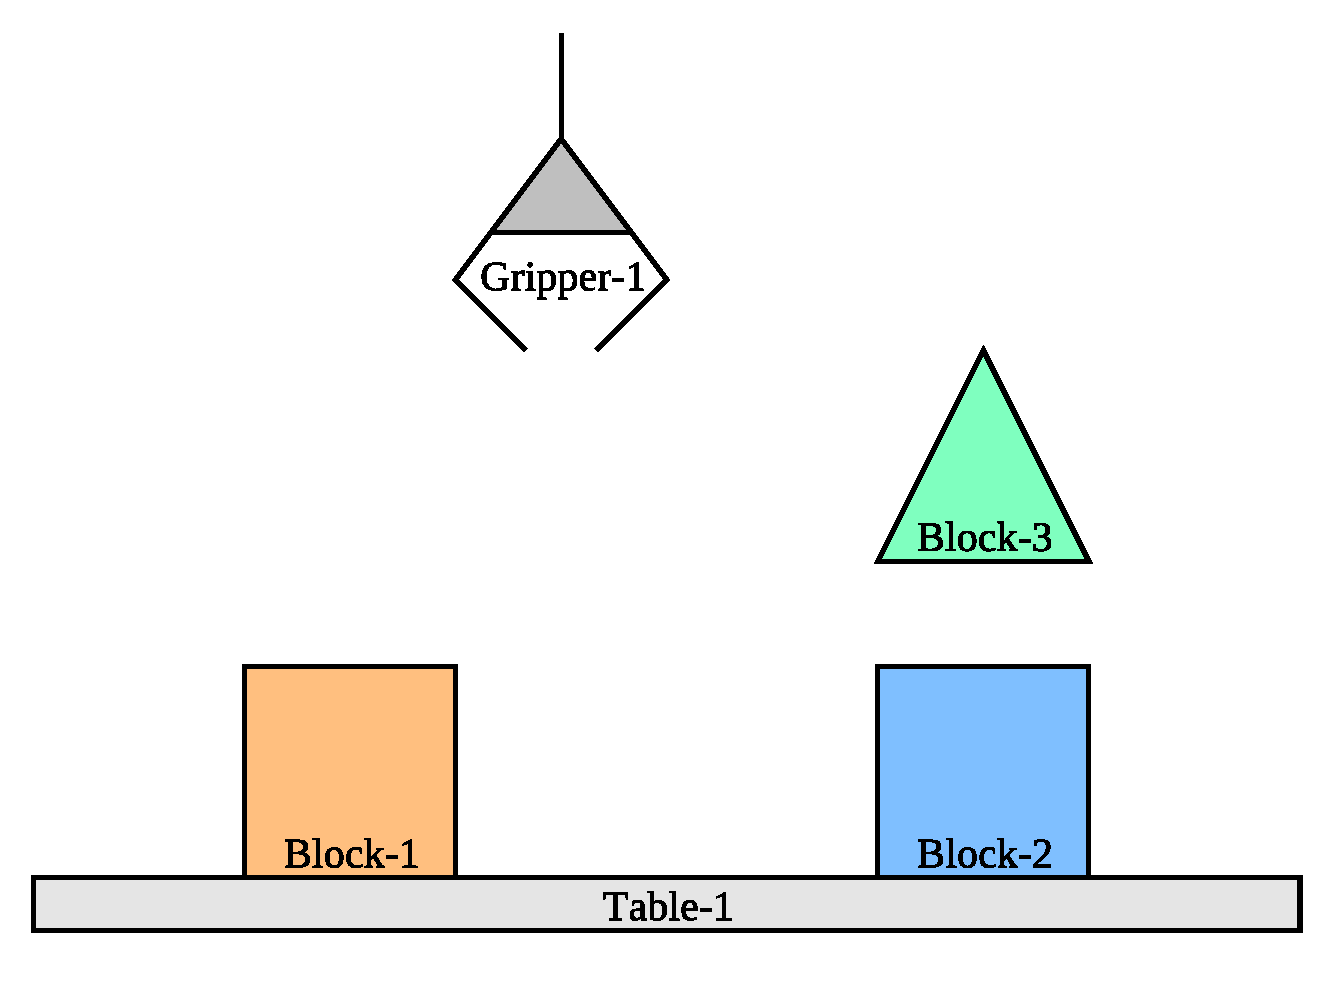
\includegraphics[width=11cm]{gfx/blocks_world_screenshot-1}
  \caption[Blocks world is a simple real-time symbolic control problem.]{Blocks world is a simple real-time symbolic control problem that I use to demonstrate my reflective control learning theory.}
  \label{fig:blocks_world_screenshot-1}
\end{figure}

I use blocks world, a canonical toy AI problem, in order to demonstrate my example of reflectively learning to plan.
See Figure~\ref{fig:blocks_world_screenshot-1} for a screenshot of my blocks world problem physical simulation.

\begin{table}
  \myfloatalign
  \begin{tabularx}{\textwidth}{XllX}
    & [Gripper-1 is me] & [Gripper-1 movement\_command []] & \\
    & [Gripper-1 is-a gripper] & [Gripper-1 color black] & \\
    & [Gripper-1 is-holding []] & [Block-1 is-a block] & \\
    & [Block-1 color brown] & [Block-1 shape cube] & \\
    & [Block-1 on Table-1] & [Block-1 left-of Gripper-1] & \\
    & [Block-2 is-a block] & [Block-2 color blue] & \\
    & [Block-2 shape cube] & [Block-2 on Table-1] & \\
    & [Block-2 right-of Gripper-1] & [Block-3 is-a block] & \\
    & [Block-3 color green] & [Block-3 shape pyramid] & \\
    & [Block-3 right-of Gripper-1] & [Table-1 is-a block] & \\
    & [Table-1 color white] & [Table-1 shape cube] & \\
    & [Table-1 left-of Gripper-1] & &
  \end{tabularx}
  \caption[Blocks world agent perceptual input.]{Blocks world agent perceptual input.}
  \label{tab:blocks_world_agent_perceptions}
\end{table}

See Table~\ref{tab:blocks_world_agent_perceptions} for an example set of perceptual input that corresponds with the physical situation shown in Figure~\ref{fig:blocks_world_screenshot-1}.

\section{Working in a World of Building Blocks}

In his PhD thesis, Terry Winograd worked in the world of building
blocks \citep{winograd:1970}.  This program maintained traces of its
goals and subgoals, which enabled it to answer questions about why it
performed certain actions.  This system worked because it stored
goals.

Knowing the goal state of the computation is important, and I do not
ignore this aspect in tracing the deliberative layer.  My system is
able to answer these sorts of questions, as this simply requires
climbing the stack of mental resource activations, but when debugging
the deliberative process, it is helpful to not only know the ending
point of computation but also the means toward that end.

\section{Terry Winograd's SHRDLU and Goal Tracing}

I am building upon what was learned from Winograd's thesis
\citep{winograd:1970} in terms of using traces of the deliberative
process as well as using a semantic model of the world in order to
understand communications between agents.  I have chosen to use a
simpler and more direct language interface between agents that refers
more directly to the semantic information and mental processes
involved.  I have experimented with implementing the original SHRDLU
english language parser, although I believe the parsing process can be
better controlled as a goal-oriented set of concurrent processes than
as the stack-based depth first search that I started writing in my
initial experiments.

\section{Why Not Work Within a Building Blocks Domain?}

The building blocks approach is a good precedent.  However, there are
many problems with only demonstrating a solution on a toy problem.
First, an approach demonstrated to solve a small problem, often do not
scale to larger problem domains of similar complexity.  So, I feel
that it is important to show the same reflective approach to learning
can also be applied to a domain with a much larger state space than
the toy blocks world problem.  I then, have shown the theoretical
gains of my approach by using the canonical model as a tool for
explanation, and now I show that my model does scale to larger
problem domains of only slightly more complexity.  See
\cite{smith:2010} for a discussion of the benefits of approaching the
social commonsense reasoning problem with a physical simulation of a
kitchen.

I have conscripted my domain of object types in the kitchen, such
that it is currently comparable to the number of object types that
Winograd used in his thesis.  My object types do have different ways
that they may be used, which is a small addition of complexity.
Although I do not introduce many of the complexities of ontological
reasoning, a common approach to commonsense reasoning, e.g. Cyc
\citep{lenat:1990}, my system demonstrates an important new approach
to commonsense reasoning that grounds learning by being told in the
domain of goal-oriented reasoning, which allows organizing and
debugging knowledge in terms of what goals it is useful for
accomplishing.

\section{A Physical Simulation of a Kitchen as a Social Commonsense Reasoning Domain}

\begin{figure}[bth]
  \center
  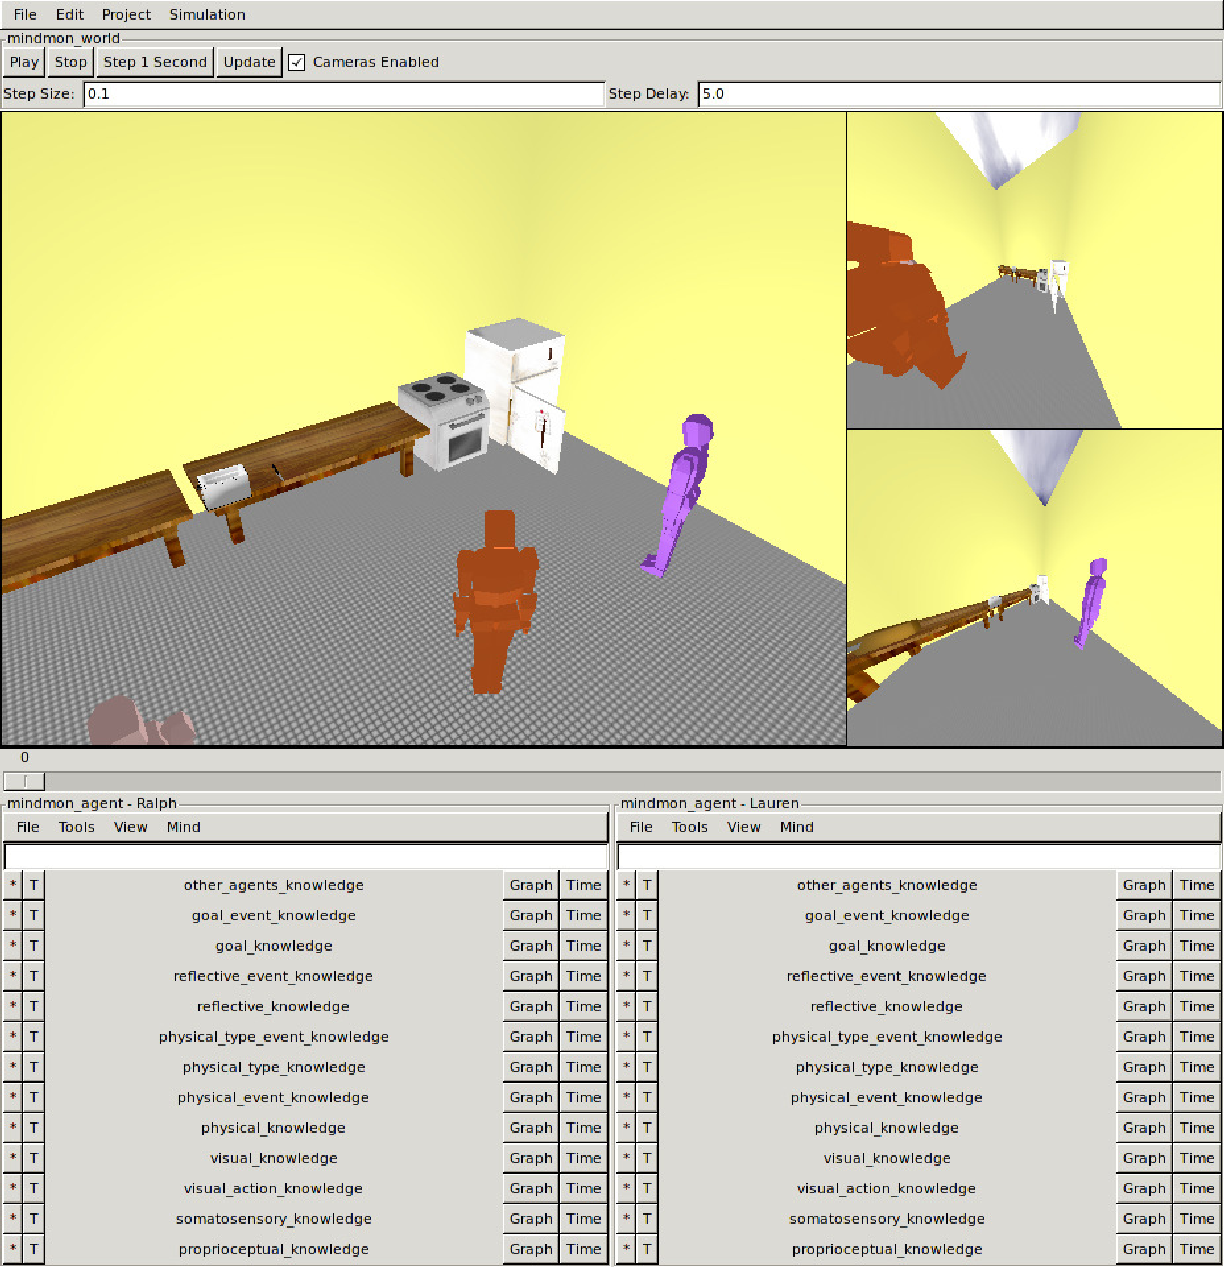
\includegraphics[width=11cm]{gfx/mindmon-isis_world-screenshot-1}
  \caption[Isis World is a larger physical simulation than the Blocks
    World toy problem.]{Isis World is a larger real-time symbolic
    physical simulation, which I use to demonstrate that my reflective
    goal-oriented learning approach scales to the physical and
    reflective problem spaces of slightly more complicated learning
    problems.}
  \label{fig:mindmon-isis_world-screenshot-1}
\end{figure}

I have experimented with applying my cognitive architecture to a
larger social commonsense reasoning domain with parents that teach
children as they attempt to accomplish cooking tasks in a kitchen.
See \cite{morgan:2011} for details about my six-layered reflective
theory of social and moral reasoning, which assumes the existence of a
procedurally reflective infrastructure with a reflective problem
solver written within it.  From an educational perspective,
\cite{dewey:1907} has theorized that kitchens are a good example of a
rich learning environment for children.  Some form of kitchen, or a
social place where food is cooked for a family, is ubiquitous across
cultures.  Kitchens have a clear production goal, namely food.  Many
mental realms must be used in accomplishing even simple cooking goals,
including: math, physics, chemistry, thermodynamics, language,
society, family, imprimer learning, concurrent planning, etc.  See
Figure~\ref{fig:mindmon-isis_world-screenshot-1} for a screenshot of
my graphical user interface to the cognitive architecture, while it
interacts with the Isis World physical simulation.


\cleardoublepage\part{Conclusion}
%*****************************************
\chapter{Results}\label{ch:results}
%*****************************************


\section{Reflective Knowledge Substrate}


\subsection{General Parallelism and Concurrency}

My system is built to handle concurrent parallel processes on
multi-core operating systems.  In this section, I test how efficient
my implementation of concurrency performs on a number of standard
concurrency timing tasks.  In an ideal situation, given $N$ processor
core working on independenct problems, I should get a factor of $N$
speedup.  Because multiple core processors share memory resources this
ideal is never actualized, so we test our implementations performance
by developing appropriate metrics.

\subsection{Program as Data}

In systems where the program is data, a bottleneck in writing programs
that write programs is the efficiency of the run-time compiler.  In
this section we test the relative performance of our compiler in
our-time system.

\section{Layered Reflective Problem Solving}

In this section, I evaluate how well different configurations of my
learning system accomplishes a range of goals in the blocks world
environment.

\subsection{Comparison between Learned Reactions and Planning}

I evaluate how adding or removing reflectively learning to plan
changes the performance of the blocks world goal accomplishment
metric.

\subsection{Analogy between Physical Goals and Planning Goals}

I evaluate how adding or removing the second layer of reflectively
learning to plan changes the performance of the blocks world goal
accomplishment metric.

\section{Learning by Credit Assignment}

\subsection{Tracing Knowledge Provenance for Credit Assignment of Success or Failure}

I evaluate how tracing causality of knowledge provenance can improve
learning performance according to the blocks world goal accomplishment
metric.


%*****************************************
\chapter{Discussion}\label{ch:discussion}
%*****************************************

During our initial experiments, we discovered many organizational
benefits of representing parts of our system in a reflectively traced
form.

\section{Reflective Knowledge Maintainance}



\section{Script Decomposition and Recomposition}


%*****************************************
\chapter{Future}\label{chapter:future}
%*****************************************

\label{section:model_6_future_research}

I began discussing strong parallels between my model and Minsky's
six-layered reflective theory of mind, called The Emotion Machine or
Model-6, in \autoref{backreference:self_reflective_self_conscious}.
Now I will continue a description of the top two layers of Minsky's
model in the theoretical terms of my model.

\section{Objective Reflection}

The ability to abstract object and subject distinctions within the
mind is key to how I see the creation of selves.  The primary object
abstractions would necessarily be based on physical activities that
lead toward or against physical goals.  An object has subjective
perspectives and extents in Space.  Further, every subjective
perspective would usefully have a set of causal hypotheses that lead
to and away from the object's more central subjective perspectives.
Objects, therefore, become collections of subjective perspectives that
can be easily traversed given the included causal models.  The extent
of an object in Space gives a useful Spatial arrangement for causal
hypotheses that help to create controllable boundaries around similar
perceptual and goal activities.

For example, this makes sense from a survivability standpoint.  The
most important and the first subject and object distinctions are those
that help accomplish or avoid physical goals.  In creating the
distinction that allows the mind to see the physical body as subjected
to the objects of a physical world, the mind has created one of the
first subjective perspectives, the physical body.

\section{Circular Objects}

Causal hypotheses are used in order to predict the future occurrence
of symbolic perceptions and goals.  Through reflective thinking, plans
are constructed from causal hypotheses consistent with the past,
elaborating the necessities in the past and the results in the future.
Analogies between consistent plans can be abstracted into models of
objects.  For example, a plan that begins and ends with the same
symbolic perception could be considered an example of a ``circular''
object; thus, an analogical plan abstraction would represent a type of
object, that has multiple sides to perceive depending on the subject's
position in the plan.  Circular objects may be an important type of
object to analogically recognize because a circular object allows one
to perform actions while being able to get back to a known perceptual
symbol.  If one is in a known circular object, then one is not lost in
the sense that one can always follow the circle in order to get back
to any perceptual symbol contained within the circular plan object.
My implementation includes tools for performing analogical
abstractions and constructions of plans, but this machinery is not key
to my thesis of explaining causal reflective learning to accomplish
goals.  I include this section in the dissertation to eliminate a
potential confusion that would conflate the concept of symbol with
that of object.  Symbols are the most primitive elements available to
thinking, while objects are more complicated in that they are composed
of analogical consistencies between plans that are themselves composed
of many symbols.  Objects have multiple subjective perspectives.
Objects are artificial creations of a mind, based on artificial static
symbols representing the ongoing activity in Duration.

\section{Body and World}

An intelligent mind builds models that predict the occurrence of
perceptual symbols.  Analogical thinking is used to abstract objects
and simultaneously the implied subjective perspectives on these
objects as they are manipulated.  The separation between the physical
body and the physical world is an objective form of thinking that is
fundamentally caused by goals that emphasize distinguishing bodily and
worldly goals in the causal structures of the physical perceptions.
For example, physical actions that change physical perceptions in
predictable ways are often bodily physical perceptions, i.e. moving
ones hand in front of ones face causes one to consistently see a hand.
Also, physical pain perceptions could be related to physical goals
that emphasize the artificial separation between the body and the
world.  Understanding the artificial separation of the body and the
world allows for an objective form of scientific study that places the
object of study in the world outside of the effects of the body.

\section{$m^\text{th}$-Stratum Objective Reflection}

Above this ability to model multiple interacting objects is the
ability to model objects as containing objects of the self-same type.
The ability to abstract all of the layers of a reflective mind into
one type of object or another can be used to recursively model one
object's model of another object.  Therefore, although my model does
not include objective reflection, I see this form of reflection as
along a new dimension that has, as its origin, all of the reflective
layers that I have so far described in my model.  I will refer to this
new dimension as ordered \emph{strata} of the \emph{objective
  dimension of reflective thinking}.

\begin{align}
\label{equation:objective_0_reflective_stratum}
\text{objective}^0\text{ reflective stratum } &{\approx} \bigcup_{n=0}^{\infty}{\text{reflective}^n\text{ layer}} \\
\label{equation:objective_m_reflective_stratum}
\text{objective}^m\text{ reflective stratum } &{\approx} \bigcup_{n=0}^{\infty}{\text{objective}^m\text{ reflective}^n\text{ layer}}
\end{align}

Prior to the first objective thinking stratum existing, it must have a
prior part of the mind upon which to objectively reflect.  I will
refer to all of the reflective layers I've described so far as the
zeroth-stratum of objective thinking, the ``$\text{objective}^0$''
stratum, since it contains no objective thinking at all.  Therefore,
the $m^\text{th}$-stratum of objective thinking in my model can be
described as ``$\text{objective}^m$'' reflective thinking.  Given this
notation, the self-reflective layer of Minsky's model would be the
first-stratum of objective thinking, or $\text{objective}^1$ reflection,
in my model.  Each $\text{objective}^m$ reflective stratum in my model
contains an infinite number of $\text{objective}^m\text{ reflective}^n$
layers.
Equations~\ref{equation:objective_0_reflective_stratum}~and~\ref{equation:objective_m_reflective_stratum},
roughly and non-mathematically show how each objective thinking
stratum is composed of an infinite number of reflective layers.
Again, this notation is \emph{not} set theoretic, and thus, set
theoretical mathematics do not apply.

\begin{figure}[bth]
  \begin{align*}
    \left.
    \begin{array}{l}
      \text{Minsky's Problem Domain }\\
      \text{Minsky's Built-in Reactive Layer }\\
      \text{Minsky's Learned Reactive Layer }\\
      \text{Minsky's Deliberative Layer }\\
      \text{Minsky's Reflective Layer }\\
    \end{array}
    \right\}                               &{\approx} \bigcup_{n=0}^{\infty}{\text{objective}^0\text{ reflective}^n\text{ layer}} \\
                                           &{\approx} \text{ objective}^0\text{ reflective stratum} \\
  \end{align*}
  \begin{align*}
    \text{Minsky's Self-Reflective Layer } &{\approx} \bigcup_{n=0}^{\infty}{\text{objective}^1\text{ reflective}^n\text{ layer}} \\
                                           &{\approx} \text{ objective}^1\text{ reflective stratum} \\
  \end{align*}
  \begin{align*}
    \text{Minsky's Self-Conscious Layer }  &{\approx} \bigcup_{n=0}^{\infty}{\text{objective}^2\text{ reflective}^n\text{ layer}} \\
                                           &{\approx} \text{ objective}^2\text{ reflective stratum}
  \end{align*}
\caption{The top layers of Model-6 roughly mapped to my
  $\text{objective}^m\text{ reflective}^n$ stratum notation.}
\label{figure:model_6_as_reflective_stratum_notation}
\end{figure}

Minsky's ``self-conscious'' layer would thereby roughly correspond
with my $\text{objective}^2$ reflective stratum.  Having two levels of
recursion in a objective thinking sense, leads to the ability to
represent what one object references in terms of what another object
references in terms of the original object.
\autoref{figure:model_6_as_reflective_stratum_notation} shows roughly
how the levels of Minsky's theory can be related to my stratum
notation.

\section{Imprimers}

\cite{minsky:2006} explains that terms like ``guilt'' and ``pride''
can refer to self-conscious ways of thinking.  Minsky hypothesizes
that there are powerful ways of thinking that result when someone whom
one respects, like a parent, values or devalues their goals.  This
type of relationship between object models is named an \emph{imprimer
  relationship} by Minsky.  In this relationship, the parent plays the
role of what Minsky has named an \emph{imprimer}, in reference to the
ability of ducklings to learn, relatively arbitrarily, to trust and
follow a parent-like figure.  Since I do not know of a another word
for an object in this sort of imprinting relationship, I will simply
use Minsky's term: imprimer.  He hypothesizes that imprimers, such as
parents and caregivers, play an important role in unquestioned
knowledge inheritance in children.  This type of thinking about what
someone else is thinking about their goals requires at least two
strata of objective reflection in my model.



% 1. models of cognition intro
% 2. literature of cognition/ commonsense (s)
% 3. problems i will solve
% 4. theory and alternatives
% 5. a system
% 6. experiments with it
% 7. discussion (how it can integrate and expand on and changes what will happen
% 8. future


%*******************************************************
% Backmatter
%*******************************************************
\appendix
\cleardoublepage\part{Appendix}
\chapter{The Code}\label{appendix:the_code}

\section{Open-Source Download}

Everything is open-source, can be downloaded from my webpage, and
compiled by simply typing "./configure; make".

\section{The Hacker Philosophy of Code}

The problems of artificial intelligence and greater control of more
complicated and interconnected computational systems are not easy
domains to approach from a programming perspective.  Many of these
problems seem to require not only new programming abstractions,
methodologies and philosophies, but also bug-free implementations of
these potentially paradigm shifting ideas.

In other words, the only people that are going to be able to solve
these types of control problems that are on the forefront of science
fiction in research are going to be expert computer programmers, or
``hackers.''  In general the ideal hacker is a problem solver that
accomplishes their own goals in given complicated systems, not
necessarily computer systems.

In terms of computational science, hackers are often confronted by
given hardware and software problems that must be overcome in order to
implement solutions to their posed problems.  Hacking can be adopted
as a fun philosophy for accomplishing ones own goals in life, but
also, I think that hacking is a required prerequisite for any form of
scientific progress.  A joy for tinkering that leads to playing, which
subsequently leaves the tinkerer as an expert hacker is what is needed
for approaching undocumented domains, such as the forefront of
artificial intelligence and control theory in general.

\section{What is a Computer?}
\label{sec:what_is_a_computer}

Good question.  We've presented a simple model in
Section~\ref{sec:state_action_model}, but this abstract model leaves a
lot to be desired for modelling the more realistic computers that most
programmers enjoy.  For example, hardware platforms with many
processing cores per CPU, multiple CPUs per motherboard, and multiple
computers per networked cluster of motherboards.  In order to
reflectively control computational systems that are organized
according to these modern engineering constraints, I have organized my
memory infrastructure to span these areas of future reflective control
research.  For example, basic pointer in the Funk2 programming
language includes 17 bits to represent the cluster machine ID, and 9
bits to represent a processor core specific memory allocation pool.
We see Funk2 as a platform supporting an open research community of
hackers that share computational resources in order to build
demonstrations of larger reflective artificial intelligence control
systems.


\section{README}

\lstset{basicstyle=\scriptsize}
\begin{lstlisting}
funk2: causally reflective programming language

  funk2 [-x <command>] [-p <portnum>] [<source.fu2>]

    <source.fu2>

        A user supplied filename of file from which to read and execute source
        code after booting and before exiting.

    -x <command>  [:default [repl]]

        A user supplied command to execute after booting and before exiting.

    -p <portnum>  [:default 22222 :try anything from 22222 to 23221]

        The localhost peer-command-server port number.  Each copy of funk2
        sharing a network interface must be able to allocate a unique
        peer-command-server port number.



TO PERFORM LOCAL BUILD:

  ./configure
  make


TO RUN LOCAL BUILD:

  ./funk2.sh    (from original compile directory)


TO PERFORM SYSTEM-WIDE INSTALLATION:

  ./configure
  make
  make install  (as root)


TO RUN SYSTEM-WIDE INSTALLATION:

  funk2         (from anywhere on system)



Homepage:

  http://funk2.org/



Git Access:

  http://git.neuromin.de/


Last Modified: 2010.10.25

Code Mass

--------------------------------------------------------------------------------

    Lines of Funk2 Code.....:   49837 total
    Words of Funk2 Code.....:  246131 total
    Characters of Funk2 Code: 2516032 total

    Lines of C Code.........:  131529 total
    Words of C Code.........:  521743 total
    Characters of C Code....: 6982294 total

    Total Lines of Code.....:  182371 total
    Total Words of Code.....:  770823 total
    Total Characters of Code: 9553461 total

--------------------------------------------------------------------------------

README Last Generated: Mon Aug  1 14:05:18 EDT 2011
\end{lstlisting}

\section{File Listing}

\lstset{basicstyle=\scriptsize}
\begin{lstlisting}
start_emacs.sh
README
configure.ac
Makefile.am
funk-mode.el
c/configurator.c
c/debugbreak.c
c/f2_agent.c
c/f2_agent.h
c/f2_ansi.c
c/f2_ansi.h
c/f2_apropos.c
c/f2_apropos.h
c/f2_archconfig.h
c/f2_array.c
c/f2_array.h
c/f2_atomic.h
c/f2_buffered_file.c
c/f2_buffered_file.h
c/f2_buffered_socket.c
c/f2_buffered_socket.h
c/f2_bug.c
c/f2_bug.h
c/f2_bytecodes.c
c/f2_bytecodes.h
c/f2_cause.c
c/f2_cause.h
c/f2_chunk.c
c/f2_chunk.h
c/f2_circular_buffer.c
c/f2_circular_buffer.h
c/f2_command_line.c
c/f2_command_line.h
c/f2_compile.c
c/f2_compile.h
c/f2_compile_x86.c
c/f2_compile_x86.h
c/f2_core_extension.c
c/f2_core_extension_funk.c
c/f2_core_extension_funk.h
c/f2_core_extension.h
c/f2_cpu.c
c/f2_cpu.h
c/f2_debug_macros.h
c/f2_dlfcn.c
c/f2_dlfcn.h
c/f2_dptr.c
c/f2_dptr.h
c/f2_dynamic_memory.c
c/f2_dynamic_memory.h
c/f2_f2ptr.c
c/f2_f2ptr.h
c/f2_fiber.c
c/f2_fiber.h
c/f2_fileio.c
c/f2_fileio.h
c/f2_frame_objects.c
c/f2_frame_objects.h
c/f2_funk2_node.c
c/f2_funk2_node.h
c/f2_funktional.c
c/f2_funktional.h
c/f2_garbage_collector.c
c/f2_garbage_collector.h
c/f2_garbage_collector_pool.c
c/f2_garbage_collector_pool.h
c/f2_globalenv.c
c/f2_globalenv.h
c/f2_global.h
c/f2_glwindow.c
c/f2_glwindow.h
c/f2_gmodule.c
c/f2_gmodule.h
c/f2_graph.c
c/f2_graph_cluster.c
c/f2_graph_cluster.h
c/f2_graph.h
c/f2_graph_match_error_correcting.c
c/f2_graph_match_error_correcting.h
c/f2_graphviz.c
c/f2_graphviz.h
c/f2_gtk.c
c/f2_gtk.h
c/f2_hash.c
c/f2_hash.h
c/f2_html.c
c/f2_html.h
c/f2_knowledge.c
c/f2_knowledge.h
c/f2_larva.c
c/f2_larva.h
c/f2_load.c
c/f2_load.h
c/f2_malloc.c
c/f2_malloc.h
c/f2_management_thread.c
c/f2_management_thread.h
c/f2_matlab.c
c/f2_matlab.h
c/f2_memblock.c
c/f2_memblock.h
c/f2_memory.c
c/f2_memory.h
c/f2_memorypool.c
c/f2_memorypool.h
c/f2_module_registration.c
c/f2_module_registration.h
c/f2_natural_language.c
c/f2_natural_language.h
c/f2_never_delete_list.c
c/f2_never_delete_list.h
c/f2_nil.c
c/f2_nil.h
c/f2_number.c
c/f2_number.h
c/f2_object.c
c/f2_object.h
c/f2_opengl.c
c/f2_opengl.h
c/f2_optimize.c
c/f2_optimize.h
c/f2_package.c
c/f2_package.h
c/f2_package_handler.c
c/f2_package_handler.h
c/f2_packet.c
c/f2_packet.h
c/f2_partial_order.c
c/f2_partial_order.h
c/f2_peer_command_server.c
c/f2_peer_command_server.h
c/f2_perception_lattice.c
c/f2_perception_lattice.h
c/f2_primes.c
c/f2_primes.h
c/f2_primfunks.c
c/f2_primfunks__errno.c
c/f2_primfunks__errno.h
c/f2_primfunks__fcntl.c
c/f2_primfunks__fcntl.h
c/f2_primfunks.h
c/f2_primfunks__ioctl.c
c/f2_primfunks__ioctl.h
c/f2_primfunks__locale.c
c/f2_primfunks__locale.h
c/f2_primfunks__string.c
c/f2_primfunks__string.h
c/f2_primobject__boolean.c
c/f2_primobject__boolean.h
c/f2_primobject__char_pointer.c
c/f2_primobject__char_pointer.h
c/f2_primobject__circular_buffer.c
c/f2_primobject__circular_buffer.h
c/f2_primobject__doublelinklist.c
c/f2_primobject__doublelinklist.h
c/f2_primobject__dynamic_library.c
c/f2_primobject__dynamic_library.h
c/f2_primobject__environment.c
c/f2_primobject__environment.h
c/f2_primobject__fiber_trigger.c
c/f2_primobject__fiber_trigger.h
c/f2_primobject__file_handle.c
c/f2_primobject__file_handle.h
c/f2_primobject__frame.c
c/f2_primobject__frame.h
c/f2_primobject__hash.c
c/f2_primobject__hash.h
c/f2_primobject__interval_tree-bak.c
c/f2_primobject__interval_tree-bak.h
c/f2_primobject__largeinteger.c
c/f2_primobject__largeinteger.h
c/f2_primobject__list.c
c/f2_primobject__list.h
c/f2_primobject__matrix.c
c/f2_primobject__matrix.h
c/f2_primobject__object.c
c/f2_primobject__object.h
c/f2_primobject__object_type.c
c/f2_primobject__object_type.h
c/f2_primobject__ptypehash.c
c/f2_primobject__ptypehash.h
c/f2_primobject__redblacktree.c
c/f2_primobject__redblacktree.h
c/f2_primobjects.c
c/f2_primobject__set.c
c/f2_primobject__set.h
c/f2_primobjects.h
c/f2_primobject__stream.c
c/f2_primobject__stream.h
c/f2_primobject__tensor.c
c/f2_primobject__tensor.h
c/f2_primobject__traced_cmutex.c
c/f2_primobject__traced_cmutex.h
c/f2_primobject_type.c
c/f2_primobject_type.h
c/f2_primobject_type_handler.c
c/f2_primobject_type_handler.h
c/f2_print.c
c/f2_print.h
c/f2_processor.c
c/f2_processor.h
c/f2_processor_mutex.c
c/f2_processor_mutex.h
c/f2_processor_thread.c
c/f2_processor_thread.h
c/f2_processor_thread_handler.c
c/f2_processor_thread_handler.h
c/f2_protected_alloc_array.c
c/f2_protected_alloc_array.h
c/f2_ptype.c
c/f2_ptype.h
c/f2_ptypes.c
c/f2_ptypes.h
c/f2_ptypes_memory.h
c/f2_reader.c
c/f2_reader.h
c/f2_redblacktree.c
c/f2_redblacktree.h
c/f2_reflective_memory.c
c/f2_scheduler.c
c/f2_scheduler.h
c/f2_scheduler_thread_controller.c
c/f2_scheduler_thread_controller.h
c/f2_search.c
c/f2_search.h
c/f2_set.c
c/f2_set.h
c/f2_signal.c
c/f2_signal.h
c/f2_simple_repl.c
c/f2_simple_repl.h
c/f2_socket.c
c/f2_socket_client.c
c/f2_socket_client.h
c/f2_socket.h
c/f2_socket_server.c
c/f2_socket_server.h
c/f2_sort.c
c/f2_sort.h
c/f2_staticmemory.c
c/f2_staticmemory.h
c/f2_status.c
c/f2_status.h
c/f2_string.c
c/f2_string.h
c/f2_surrogate_parent.c
c/f2_surrogate_parent.h
c/f2_system_file_handler.c
c/f2_system_file_handler.h
c/f2_system_headers.h
c/f2_system_processor.c
c/f2_system_processor.h
c/f2_terminal_print.c
c/f2_terminal_print.h
c/f2_termios.c
c/f2_termios.h
c/f2_time.c
c/f2_time.h
c/f2_trace.c
c/f2_trace.h
c/f2_tricolor_set.c
c/f2_tricolor_set.h
c/f2_user_thread_controller.c
c/f2_user_thread_controller.h
c/f2_virtual_processor.c
c/f2_virtual_processor.h
c/f2_virtual_processor_handler.c
c/f2_virtual_processor_handler.h
c/f2_virtual_processor_thread.c
c/f2_virtual_processor_thread.h
c/f2_xmlrpc.c
c/f2_xmlrpc.h
c/f2_zlib.c
c/f2_zlib.h
c/funk2.c
c/funk2.h
c/funk2_main.c
c/test.c
fu2/action.fu2
fu2/actor.fu2
fu2/actortest.fu2
fu2/assembler.fu2
fu2/bootstrap-apropos.fu2
fu2/bootstrap-array.fu2
fu2/bootstrap-boot.fu2
fu2/bootstrap-bug.fu2
fu2/bootstrap-bugs.fu2
fu2/bootstrap-cause.fu2
fu2/bootstrap-compound_object.fu2
fu2/bootstrap-cons.fu2
fu2/bootstrap-core_extension.fu2
fu2/bootstrap-core_extension_funk.fu2
fu2/bootstrap-critic.fu2
fu2/bootstrap-critics-reactive.fu2
fu2/bootstrap-default_critics.fu2
fu2/bootstrap-define_bug_responses.fu2
fu2/bootstrap-dynamic_library.fu2
fu2/bootstrap-fiber.fu2
fu2/bootstrap-frame.fu2
fu2/bootstrap.fu2
fu2/bootstrap-garbage_collector.fu2
fu2/bootstrap-graph.fu2
fu2/bootstrap-graph-old.fu2
fu2/bootstrap-grid.fu2
fu2/bootstrap-hash.fu2
fu2/bootstrap-largeinteger.fu2
fu2/bootstrap-list.fu2
fu2/bootstrap-object.fu2
fu2/bootstrap-package.fu2
fu2/bootstrap-primobject.fu2
fu2/bootstrap-ptypes.fu2
fu2/bootstrap-reader.fu2
fu2/bootstrap-redblacktree.fu2
fu2/bootstrap-repl.fu2
fu2/bootstrap-set_theory.fu2
fu2/bootstrap-sort.fu2
fu2/bootstrap-string.fu2
fu2/bootstrap-surrogate_parent.fu2
fu2/bootstrap-terminal_print.fu2
fu2/bootstrap-type_conversions.fu2
fu2/bootstrap-zlib.fu2
fu2/brainviz.fu2
fu2/cardgame-ai.fu2
fu2/cardgame.fu2
fu2/cause.fu2
fu2/characters.fu2
fu2/compile.fu2
fu2/emailcharacters.fu2
fu2/emotionmachine.fu2
fu2/english-eval.fu2
fu2/graph.fu2
fu2/graph_match_test.fu2
fu2/graphviz.fu2
fu2/internet.fu2
fu2/link-grammar-wrapper.fu2
fu2/miscfunks.fu2
fu2/neuralmom-brain_area.fu2
fu2/neuralmom-demo.fu2
fu2/neuralmom-nervous_system.fu2
fu2/neuralmom-occipital_cortex.fu2
fu2/opengl.fu2
fu2/pattern.fu2
fu2/planner.fu2
fu2/primfunks-apropos.fu2
fu2/primfunks-arithmetic.fu2
fu2/primfunks-array.fu2
fu2/primfunks-bug.fu2
fu2/primfunks-cause.fu2
fu2/primfunks-chunk.fu2
fu2/primfunks-compile.fu2
fu2/primfunks-core_extension.fu2
fu2/primfunks-core_extension_funk.fu2
fu2/primfunks-cpu.fu2
fu2/primfunks-dlfcn.fu2
fu2/primfunks-errno.fu2
fu2/primfunks-fcntl.fu2
fu2/primfunks-fiber.fu2
fu2/primfunks-fiber_trigger.fu2
fu2/primfunks-frame.fu2
fu2/primfunks.fu2
fu2/primfunks-garbage_collector.fu2
fu2/primfunks-gmodule.fu2
fu2/primfunks-graph.fu2
fu2/primfunks-hash.fu2
fu2/primfunks-ioctl.fu2
fu2/primfunks-largeinteger.fu2
fu2/primfunks-locale.fu2
fu2/primfunks-management_thread.fu2
fu2/primfunks-object.fu2
fu2/primfunks-optimize.fu2
fu2/primfunks-package.fu2
fu2/primfunks-package_handler.fu2
fu2/primfunks-primes.fu2
fu2/primfunks-primobjects.fu2
fu2/primfunks-primobject_type.fu2
fu2/primfunks-primobject_type_handler.fu2
fu2/primfunks-print.fu2
fu2/primfunks-ptypes.fu2
fu2/primfunks-reader.fu2
fu2/primfunks-redblacktree.fu2
fu2/primfunks-scheduler.fu2
fu2/primfunks-search.fu2
fu2/primfunks-set.fu2
fu2/primfunks-socket.fu2
fu2/primfunks-sort.fu2
fu2/primfunks-string.fu2
fu2/primfunks-surrogate_parent.fu2
fu2/primfunks-terminal_print.fu2
fu2/primfunks-termios.fu2
fu2/primfunks-time.fu2
fu2/primfunks-trace.fu2
fu2/primfunks-virtual_processor_handler.fu2
fu2/primfunks-zlib.fu2
fu2/reactive.fu2
fu2/readline-wrapper.fu2
fu2/repl.fu2
fu2/rlglue-wrapper.fu2
fu2/serialize.fu2
fu2/story.fu2
fu2/thought_process.fu2
fu2/trace.fu2
fu2/x86-compile.fu2
fu2/x86-compile-machine_code.fu2
fu2/x86-compile-mov.fu2
misc/fables.fu2
misc/frog_and_toad.fu2
misc/frog-and-toad.fu2
misc/officer_joke.fu2
misc/roboverse-blocks_world.fu2
misc/roboverse-demo.fu2
misc/simple_game.fu2
extension/cairo/cairo.c
extension/cairo/cairo.h
extension/causality/causality.c
extension/conceptnet/conceptnet.c
extension/conceptnet/conceptnet.h
extension/concept_version_space/concept_version_space.c
extension/concept_version_space/concept_version_space.h
extension/equals_hash/equals_hash.c
extension/equals_hash/equals_hash.h
extension/event_stream/event_stream.c
extension/event_stream/event_stream.h
extension/fibermon/fibermon.c
extension/forgetful_event_stream/forgetful_event_stream.c
extension/forgetful_event_stream/forgetful_event_stream.h
extension/forward_planner/forward_planner.c
extension/frame_ball/frame_ball.c
extension/graph_isomorphism/graph_isomorphism.c
extension/graph_isomorphism/graph_isomorphism.h
extension/image/image.c
extension/image/image.h
extension/image_sequence/image_sequence.c
extension/image_sequence/image_sequence.h
extension/interval_tree/interval_tree.c
extension/interval_tree/interval_tree.h
extension/lick/lick.c
extension/lick/lick.h
extension/mentality/mentality.c
extension/mentality/mentality.h
extension/meta_semantic_knowledge_base/meta_semantic_knowledge_base.c
extension/meta_semantic_knowledge_base/meta_semantic_knowledge_base.h
extension/movie/movie.c
extension/movie/movie.h
extension/propogator/propogator.c
extension/propogator/propogator.h
extension/semantic_action_event/semantic_action_event.c
extension/semantic_action_event/semantic_action_event.h
extension/semantic_agent/semantic_agent.c
extension/semantic_agent/semantic_agent.h
extension/semantic_category/semantic_category.c
extension/semantic_category/semantic_category.h
extension/semantic_causal_event/semantic_causal_event.c
extension/semantic_causal_event/semantic_causal_event.h
extension/semantic_causal_object/semantic_causal_object.c
extension/semantic_causal_object/semantic_causal_object.h
extension/semantic_containment_object/semantic_containment_object.c
extension/semantic_containment_object/semantic_containment_object.h
extension/semantic_directed_action_event/semantic_directed_action_event.c
extension/semantic_directed_action_event/semantic_directed_action_event.h
extension/semantic_event_knowledge_base/semantic_event_knowledge_base.c
extension/semantic_event_knowledge_base/semantic_event_knowledge_base.h
extension/semantic_event/semantic_event.c
extension/semantic_event/semantic_event.h
extension/semantic_event_sequence/semantic_event_sequence.c
extension/semantic_event_sequence/semantic_event_sequence.h
extension/semantic_event_tree/semantic_event_tree.c
extension/semantic_event_tree/semantic_event_tree.h
extension/semantic_frame/semantic_frame.c
extension/semantic_frame/semantic_frame.h
extension/semantic_goal_action_causal_hypothesis/semantic_goal_action_causal_hypothesis.c
extension/semantic_goal_action_causal_hypothesis/semantic_goal_action_causal_hypothesis.h
extension/semantic_goal/semantic_goal.c
extension/semantic_goal/semantic_goal.h
extension/semantic_knowledge_base/semantic_knowledge_base.c
extension/semantic_knowledge_base/semantic_knowledge_base.h
extension/semantic_know_of_existence_event/semantic_know_of_existence_event.c
extension/semantic_know_of_existence_event/semantic_know_of_existence_event.h
extension/semantic_know_of_relationship_event/semantic_know_of_relationship_event.c
extension/semantic_know_of_relationship_event/semantic_know_of_relationship_event.h
extension/semantic_object/semantic_object.c
extension/semantic_object/semantic_object.h
extension/semantic_object_type/semantic_object_type.c
extension/semantic_object_type/semantic_object_type.h
extension/semantic_ordered_object/semantic_ordered_object.c
extension/semantic_ordered_object/semantic_ordered_object.h
extension/semantic_packable_object/semantic_packable_object.c
extension/semantic_packable_object/semantic_packable_object.h
extension/semantic_physical_object/semantic_physical_object.c
extension/semantic_physical_object/semantic_physical_object.h
extension/semantic_physical_object_type_relation/semantic_physical_object_type_relation.c
extension/semantic_physical_object_type_relation/semantic_physical_object_type_relation.h
extension/semantic_physical_object_type/semantic_physical_object_type.c
extension/semantic_physical_object_type/semantic_physical_object_type.h
extension/semantic_proprioception/semantic_proprioception.c
extension/semantic_proprioception/semantic_proprioception.h
extension/semantic_proprioceptual_object/semantic_proprioceptual_object.c
extension/semantic_proprioceptual_object/semantic_proprioceptual_object.h
extension/semantic_proprioceptual_orientation/semantic_proprioceptual_orientation.c
extension/semantic_proprioceptual_orientation/semantic_proprioceptual_orientation.h
extension/semantic_proprioceptual_position/semantic_proprioceptual_position.c
extension/semantic_proprioceptual_position/semantic_proprioceptual_position.h
extension/semantic_realm/semantic_realm.c
extension/semantic_realm/semantic_realm.h
extension/semantic_relationship_key/semantic_relationship_key.c
extension/semantic_relationship_key/semantic_relationship_key.h
extension/semantic_resource_action_event/semantic_resource_action_event.c
extension/semantic_resource_action_event/semantic_resource_action_event.h
extension/semantic_resource_action_sequence/semantic_resource_action_sequence.c
extension/semantic_resource_action_sequence/semantic_resource_action_sequence.h
extension/semantic_resource_event_knowledge_base/semantic_resource_event_knowledge_base.c
extension/semantic_resource_event_knowledge_base/semantic_resource_event_knowledge_base.h
extension/semantic_resource/semantic_resource.c
extension/semantic_resource/semantic_resource.h
extension/semantic_self/semantic_self.c
extension/semantic_self/semantic_self.h
extension/semantic_situation_category/semantic_situation_category.c
extension/semantic_situation_category/semantic_situation_category.h
extension/semantic_situation/semantic_situation.c
extension/semantic_situation/semantic_situation.h
extension/semantic_situation_transition/semantic_situation_transition.c
extension/semantic_situation_transition/semantic_situation_transition.h
extension/semantic_somatosensation/semantic_somatosensation.c
extension/semantic_somatosensation/semantic_somatosensation.h
extension/semantic_somatosensory_object/semantic_somatosensory_object.c
extension/semantic_somatosensory_object/semantic_somatosensory_object.h
extension/semantic_temporal_object/semantic_temporal_object.c
extension/semantic_temporal_object/semantic_temporal_object.h
extension/semantic_time/semantic_time.c
extension/semantic_time/semantic_time.h
extension/semantic_visual_object/semantic_visual_object.c
extension/semantic_visual_object/semantic_visual_object.h
extension/timeline/timeline.c
extension/timeline/timeline.h
built-in/alien/alien.fu2
built-in/ansi/primfunks-ansi.fu2
built-in/basic_bug_responses/basic_bug_responses.fu2
built-in/graph_cluster/bootstrap-graph_cluster.fu2
built-in/graph_cluster/primfunks-graph_cluster.fu2
built-in/graph_match_error_correcting/graph_match_error_correcting.fu2
built-in/graph_match_error_correcting/graph_match_error_correcting-primfunks.fu2
built-in/graphviz/graphviz.fu2
built-in/graphviz/graphviz-primfunks.fu2
built-in/gtk/bootstrap-gtk.fu2
built-in/gtk/primfunks-gtk.fu2
built-in/math/math.fu2
built-in/mutex/mutex.fu2
built-in/natural_language/dictionary_frame.fu2
built-in/natural_language/natural_language_command.fu2
built-in/natural_language/natural_language-primfunks.fu2
built-in/natural_language/parse_tree.fu2
built-in/natural_language/skb-test.fu2
built-in/number/bootstrap-number.fu2
built-in/number/primfunks-number.fu2
built-in/object_lattice/bootstrap-object_lattice.fu2
built-in/object_lattice/primfunks-object_lattice.fu2
built-in/perception_lattice/bootstrap-perception_lattice.fu2
built-in/perception_lattice/primfunks-perception_lattice.fu2
built-in/utilities/errno.fu2
built-in/utilities/fcntl.fu2
built-in/utilities/ioctl.fu2
built-in/utilities/socket.fu2
built-in/xmlrpc/bootstrap-xmlrpc.fu2
built-in/xmlrpc/primfunks-xmlrpc.fu2
example/blocks_world/blocks_world_block.fu2
example/blocks_world/blocks_world.fu2
example/blocks_world/blocks_world_gripper_controller.fu2
example/blocks_world/blocks_world_gripper.fu2
example/blocks_world/blocks_world_physics.fu2
example/blocks_world/blocks_world_sprite.fu2
example/blocks_world/blocks_world_window.fu2
example/divisi2/divisi2.fu2
example/em_two_webpage/em_two_webpage.fu2
example/english_language/english_dictionary.fu2
example/english_language/english_dictionary_parse.fu2
example/funk2-htmldoc/funk2-htmldoc.fu2
example/funk2-webpage/funk2-webpage.fu2
example/graph_match/graph_match.fu2
example/graph_match/graph_match-test.fu2
example/gtk_timeline/gtk_timeline.fu2
example/isismon/isismon_agent.fu2
example/isismon/isismon_builtin_reactive_physical_activator.fu2
example/isismon/isismon_deliberative_forward_planner_activator.fu2
example/isismon/isismon_deliberative_goal_activator.fu2
example/isismon/isismon.fu2
example/isismon/isismon_knowledge.fu2
example/isismon/isismon_learned_reactive_physical_activator.fu2
example/isis_world_client/isis_world_client.fu2
example/isis_world_demo/isis_agent_body.fu2
example/isis_world_demo/isis_visual_agent.fu2
example/isis_world_demo/isis_visual_object.fu2
example/isis_world_demo/isis_world_demo.fu2
example/isis_world_demo/isis_world.fu2
example/isis_world_demo/jj.fu2
example/little_carol_world/little_carol_world.fu2
example/macbeth/macbeth.fu2
example/mind/agency.fu2
example/mind/agent_body.fu2
example/mind/character.fu2
example/mind/mental_layer.fu2
example/mind/mind.fu2
example/mindmon-1.0/mindmon-1.0.fu2
example/mindmon-blocks_world/mindmon-blocks_world.fu2
example/mindmon-isis_world/mindmon-isis_world-builtin_reactive_physical_activator.fu2
example/mindmon-isis_world/mindmon-isis_world-deliberative_goal_activator.fu2
example/mindmon-isis_world/mindmon-isis_world.fu2
example/mindmon-isis_world/mindmon-isis_world-learned_reactive_physical_activator.fu2
example/mindmon/mindmon_agent.fu2
example/mindmon/mindmon_agent_tool.fu2
example/mindmon/mindmon_agent_tool_widget.fu2
example/mindmon/mindmon_agent_widget.fu2
example/mindmon/mindmon.fu2
example/mindmon/mindmon_knowledge.fu2
example/mindmon/mindmon_world.fu2
example/mind/physical_world.fu2
example/mind/resource.fu2
example/mind/self_model.fu2
example/mind/story.fu2
example/mind/story-graph.fu2
example/moral_compass-isis_world/moral_compass-isis_world-builtin_reactive_physical_agency_resources.fu2
example/moral_compass-isis_world/moral_compass-isis_world.fu2
example/moral_compass-isis_world/moral_compass-isis_world-learned_reactive_physical_agency_resources.fu2
example/moral_compass-isis_world/moral_compass-isis_world-learned_reactive_physical_agency_resources-functions.fu2
example/moral_compass/moral_agent_body.fu2
example/moral_compass/moral_compass.fu2
example/moral_compass/old_reflective_event_knowledge_agency-bak.fu2
example/moral_compass/self_conscious_imprimer_agency.fu2
example/moral_compass/self_conscious_layer.fu2
example/moral_compass/self_reflective_layer.fu2
example/moral_compass/self_reflective_other_agents_knowledge_agency.fu2
example/muddy_carol/muddy_carol.fu2
example/rct_webpage/rct_webpage.fu2
example/reflective_mind-blocks_world/reflective_mind-blocks_world.fu2
example/reflective_mind/builtin_reactive_layer.fu2
example/reflective_mind/builtin_reactive_neural_plug_agency.fu2
example/reflective_mind/builtin_reactive_physical_agency.fu2
example/reflective_mind/builtin_reactive_sensory_agency.fu2
example/reflective_mind/deliberative_execution_agency.fu2
example/reflective_mind/deliberative_forward_planner_agency.fu2
example/reflective_mind/deliberative_forward_planner_agency-test.fu2
example/reflective_mind/deliberative_goal_creation_agency.fu2
example/reflective_mind/deliberative_goal_event_knowledge_agency.fu2
example/reflective_mind/deliberative_goal_knowledge_agency.fu2
example/reflective_mind/deliberative_layer.fu2
example/reflective_mind/deliberative_physical_event_knowledge_agency.fu2
example/reflective_mind/learned_reactive_language_agency.fu2
example/reflective_mind/learned_reactive_layer.fu2
example/reflective_mind/learned_reactive_physical_agency.fu2
example/reflective_mind/learned_reactive_physical_knowledge_agency.fu2
example/reflective_mind/learned_reactive_sensory_agency.fu2
example/reflective_mind/reflective_credit_assignment_agency.fu2
example/reflective_mind/reflective_event_knowledge_agency.fu2
example/reflective_mind/reflective_layer.fu2
example/reflective_mind/reflective_mind.fu2
example/reflective_mind/reflective_mind_perception.fu2
example/reflective_mind/reflective_mind_proprioceptual_object.fu2
example/reflective_mind/reflective_mind_visual_agent.fu2
example/reflective_mind/reflective_mind_visual_object.fu2
example/roboverse/roboverse.fu2
example/socket-client/socket-client.fu2
example/socket-server/socket-server.fu2
example/traced_mind/traced_mind.fu2
example/traced_mind/traced_resource.fu2
example/visualize/isismon_agent_visualization.fu2
example/visualize/visualize_test.fu2
extension/cairo/cairo-core.fu2
extension/conceptnet/conceptnet-core.fu2
extension/concept_version_space/concept_version_space-core.fu2
extension/equals_hash/equals_hash-core.fu2
extension/event_stream/event_stream-core.fu2
extension/fibermon/fibermon1.fu2
extension/fibermon/fibermon-core.fu2
extension/fibermon/fibermon.fu2
extension/forgetful_event_stream/forgetful_event_stream-core.fu2
extension/forward_planner/forward_planner-core.fu2
extension/frame_ball/frame_ball-core.fu2
extension/graph_isomorphism/graph_isomorphism-core.fu2
extension/image/image-core.fu2
extension/image_sequence/image_sequence-core.fu2
extension/interval_tree/interval_tree-core.fu2
extension/lick/lick-core.fu2
extension/mentality/mentality-core.fu2
extension/meta_semantic_knowledge_base/meta_semantic_knowledge_base-core.fu2
extension/movie/movie-core.fu2
extension/propogator/propogator-core.fu2
extension/semantic_action_event/semantic_action_event-core.fu2
extension/semantic_agent/semantic_agent-core.fu2
extension/semantic_category/semantic_category-core.fu2
extension/semantic_causal_event/semantic_causal_event-core.fu2
extension/semantic_causal_object/semantic_causal_object-core.fu2
extension/semantic_containment_object/semantic_containment_object-core.fu2
extension/semantic_directed_action_event/semantic_directed_action_event-core.fu2
extension/semantic_event_knowledge_base/semantic_event_knowledge_base-core.fu2
extension/semantic_event/semantic_event-core.fu2
extension/semantic_event_sequence/semantic_event_sequence-core.fu2
extension/semantic_event_tree/semantic_event_tree-core.fu2
extension/semantic_frame/semantic_frame-core.fu2
extension/semantic_goal_action_causal_hypothesis/semantic_goal_action_causal_hypothesis-core.fu2
extension/semantic_goal/semantic_goal-core.fu2
extension/semantic_knowledge_base/semantic_knowledge_base-core.fu2
extension/semantic_know_of_existence_event/semantic_know_of_existence_event-core.fu2
extension/semantic_know_of_relationship_event/semantic_know_of_relationship_event-core.fu2
extension/semantic_object/semantic_object-core.fu2
extension/semantic_object_type/semantic_object_type-core.fu2
extension/semantic_ordered_object/semantic_ordered_object-core.fu2
extension/semantic_packable_object/semantic_packable_object-core.fu2
extension/semantic_physical_object/semantic_physical_object-core.fu2
extension/semantic_physical_object_type_relation/semantic_physical_object_type_relation-core.fu2
extension/semantic_physical_object_type/semantic_physical_object_type-core.fu2
extension/semantic_proprioception/semantic_proprioception-core.fu2
extension/semantic_proprioceptual_object/semantic_proprioceptual_object-core.fu2
extension/semantic_proprioceptual_orientation/semantic_proprioceptual_orientation-core.fu2
extension/semantic_proprioceptual_position/semantic_proprioceptual_position-core.fu2
extension/semantic_realm/semantic_realm-core.fu2
extension/semantic_relationship_key/semantic_relationship_key-core.fu2
extension/semantic_resource_action_event/semantic_resource_action_event-core.fu2
extension/semantic_resource_action_sequence/semantic_resource_action_sequence-core.fu2
extension/semantic_resource_event_knowledge_base/semantic_resource_event_knowledge_base-core.fu2
extension/semantic_resource/semantic_resource-core.fu2
extension/semantic_self/semantic_self-core.fu2
extension/semantic_situation_category/semantic_situation_category-core.fu2
extension/semantic_situation/semantic_situation-core.fu2
extension/semantic_situation_transition/semantic_situation_transition-core.fu2
extension/semantic_somatosensation/semantic_somatosensation-core.fu2
extension/semantic_somatosensory_object/semantic_somatosensory_object-core.fu2
extension/semantic_temporal_object/semantic_temporal_object-core.fu2
extension/semantic_time/semantic_time-core.fu2
extension/semantic_visual_object/semantic_visual_object-core.fu2
extension/timeline/timeline-core.fu2
test/cairo-test/cairo-test.fu2
test/concept_version_space-test/concept_version_space-test.fu2
test/gtk-test/gtk-test.fu2
test/interval_tree-test/interval_tree-test.fu2
test/optimize-test/optimize-test.fu2
test/propogator-test/propogator-test.fu2
test/timeline-test/timeline-test.fu2
test/xmlrpc-test/xmlrpc-test.fu2
built-in/alien/alien.fpkg
built-in/ansi/ansi.fpkg
built-in/basic_bug_responses/basic_bug_responses.fpkg
built-in/graph_cluster/graph_cluster.fpkg
built-in/graph_match_error_correcting/graph_match_error_correcting.fpkg
built-in/graphviz/graphviz.fpkg
built-in/gtk/gtk.fpkg
built-in/math/math.fpkg
built-in/mutex/mutex.fpkg
built-in/natural_language/natural_language.fpkg
built-in/number/number.fpkg
built-in/object_lattice/object_lattice.fpkg
built-in/perception_lattice/perception_lattice.fpkg
built-in/utilities/utilities.fpkg
built-in/xmlrpc/xmlrpc.fpkg
example/blocks_world/blocks_world.fpkg
example/divisi2/divisi2.fpkg
example/em_two_webpage/em_two_webpage.fpkg
example/english_language/english_language.fpkg
example/funk2-htmldoc/funk2-htmldoc.fpkg
example/funk2-webpage/funk2-webpage.fpkg
example/graph_match/graph_match.fpkg
example/graph_match/graph_match-test.fpkg
example/gtk_timeline/gtk_timeline.fpkg
example/isismon/isismon.fpkg
example/isis_world_client/isis_world_client.fpkg
example/isis_world_demo/isis_world_demo.fpkg
example/little_carol_world/little_carol_world.fpkg
example/macbeth/macbeth.fpkg
example/mind/mind.fpkg
example/mindmon-1.0/mindmon-1.0.fpkg
example/mindmon-blocks_world/mindmon-blocks_world.fpkg
example/mindmon-isis_world/mindmon-isis_world.fpkg
example/mindmon/mindmon.fpkg
example/moral_compass-isis_world/moral_compass-isis_world.fpkg
example/moral_compass/moral_compass.fpkg
example/muddy_carol/muddy_carol.fpkg
example/rct_webpage/rct_webpage.fpkg
example/reflective_mind-blocks_world/reflective_mind-blocks_world.fpkg
example/reflective_mind/reflective_mind.fpkg
example/roboverse/roboverse.fpkg
example/socket-client/socket-client.fpkg
example/socket-server/socket-server.fpkg
example/traced_mind/traced_mind.fpkg
example/visualize/isismon_agent_visualization.fpkg
example/visualize/visualize_test.fpkg
extension/cairo/cairo.fpkg
extension/conceptnet/conceptnet.fpkg
extension/concept_version_space/concept_version_space.fpkg
extension/equals_hash/equals_hash.fpkg
extension/event_stream/event_stream.fpkg
extension/fibermon/fibermon.fpkg
extension/forgetful_event_stream/forgetful_event_stream.fpkg
extension/forward_planner/forward_planner.fpkg
extension/frame_ball/frame_ball.fpkg
extension/graph_isomorphism/graph_isomorphism.fpkg
extension/image/image.fpkg
extension/image_sequence/image_sequence.fpkg
extension/interval_tree/interval_tree.fpkg
extension/lick/lick.fpkg
extension/mentality/mentality.fpkg
extension/meta_semantic_knowledge_base/meta_semantic_knowledge_base.fpkg
extension/movie/movie.fpkg
extension/propogator/propogator.fpkg
extension/semantic_action_event/semantic_action_event.fpkg
extension/semantic_agent/semantic_agent.fpkg
extension/semantic_category/semantic_category.fpkg
extension/semantic_causal_event/semantic_causal_event.fpkg
extension/semantic_causal_object/semantic_causal_object.fpkg
extension/semantic_containment_object/semantic_containment_object.fpkg
extension/semantic_directed_action_event/semantic_directed_action_event.fpkg
extension/semantic_event_knowledge_base/semantic_event_knowledge_base.fpkg
extension/semantic_event/semantic_event.fpkg
extension/semantic_event_sequence/semantic_event_sequence.fpkg
extension/semantic_event_tree/semantic_event_tree.fpkg
extension/semantic_frame/semantic_frame.fpkg
extension/semantic_goal_action_causal_hypothesis/semantic_goal_action_causal_hypothesis.fpkg
extension/semantic_goal/semantic_goal.fpkg
extension/semantic_knowledge_base/semantic_knowledge_base.fpkg
extension/semantic_know_of_existence_event/semantic_know_of_existence_event.fpkg
extension/semantic_know_of_relationship_event/semantic_know_of_relationship_event.fpkg
extension/semantic_object/semantic_object.fpkg
extension/semantic_object_type/semantic_object_type.fpkg
extension/semantic_ordered_object/semantic_ordered_object.fpkg
extension/semantic_packable_object/semantic_packable_object.fpkg
extension/semantic_physical_object/semantic_physical_object.fpkg
extension/semantic_physical_object_type_relation/semantic_physical_object_type_relation.fpkg
extension/semantic_physical_object_type/semantic_physical_object_type.fpkg
extension/semantic_proprioception/semantic_proprioception.fpkg
extension/semantic_proprioceptual_object/semantic_proprioceptual_object.fpkg
extension/semantic_proprioceptual_orientation/semantic_proprioceptual_orientation.fpkg
extension/semantic_proprioceptual_position/semantic_proprioceptual_position.fpkg
extension/semantic_realm/semantic_realm.fpkg
extension/semantic_relationship_key/semantic_relationship_key.fpkg
extension/semantic_resource_action_event/semantic_resource_action_event.fpkg
extension/semantic_resource_action_sequence/semantic_resource_action_sequence.fpkg
extension/semantic_resource_event_knowledge_base/semantic_resource_event_knowledge_base.fpkg
extension/semantic_resource/semantic_resource.fpkg
extension/semantic_self/semantic_self.fpkg
extension/semantic_situation_category/semantic_situation_category.fpkg
extension/semantic_situation/semantic_situation.fpkg
extension/semantic_situation_transition/semantic_situation_transition.fpkg
extension/semantic_somatosensation/semantic_somatosensation.fpkg
extension/semantic_somatosensory_object/semantic_somatosensory_object.fpkg
extension/semantic_temporal_object/semantic_temporal_object.fpkg
extension/semantic_time/semantic_time.fpkg
extension/semantic_visual_object/semantic_visual_object.fpkg
extension/timeline/timeline.fpkg
test/cairo-test/cairo-test.fpkg
test/concept_version_space-test/concept_version_space-test.fpkg
test/gtk-test/gtk-test.fpkg
test/interval_tree-test/interval_tree-test.fpkg
test/optimize-test/optimize-test.fpkg
test/propogator-test/propogator-test.fpkg
test/timeline-test/timeline-test.fpkg
test/xmlrpc-test/xmlrpc-test.fpkg
example/visualize/framework.py
example/visualize/globalvars.py
example/visualize/graphics.py
example/visualize/graphics_testing.py
example/visualize/physics.py
example/visualize/vector.py
example/visualize/visualization.py
example/visualize/xmlclient.py
example/visualize/xmlserver.py
python/funk2module/setup.py
\end{lstlisting}

%*******************************************************
% Other Stuff in the Back
%*******************************************************
\cleardoublepage%********************************************************************
% Bibliography
%*******************************************************
% work-around to have small caps also here in the headline
\manualmark
\markboth{\spacedlowsmallcaps{\bibname}}{\spacedlowsmallcaps{\bibname}} % work-around to have small caps also
%\phantomsection 
\refstepcounter{dummy}
\addtocontents{toc}{\protect\vspace{\beforebibskip}} % to have the bib a bit from the rest in the toc
\addcontentsline{toc}{chapter}{\tocEntry{\bibname}}
\bibliographystyle{agsm}
%\bibliographystyle{authordate1}
\label{app:bibliography} 
\bibliography{bibliography}

\cleardoublepage\pagestyle{empty}

\hfill

\vfill


\pdfbookmark[0]{Colophon}{colophon}
\section*{Colophon}
This thesis was typeset with \LaTeXe\ using Hermann Zapf's
\emph{Palatino}
and \emph{Euler} type faces (Type~1 PostScript fonts \emph{URW
Palladio L}
and \emph{FPL} were used). The listings are typeset in \emph{Bera
Mono}, originally developed by Bitstream, Inc. as ``Bitstream Vera''.
(Type~1 PostScript fonts were made available by Malte Rosenau and
Ulrich Dirr.)

The typographic style was inspired by Bringhurst's genius as
presented in \emph{The Elements of Typographic Style} 
(Bringhurst 2002). It is available for \LaTeX\ via \textsmaller{CTAN} as 
``\href{http://www.ctan.org/tex-archive/macros/latex/contrib/classicthesis/}%
{\texttt{classicthesis}}''.

\paragraph{note:} The custom size of the textblock was calculated
using the directions given by Mr. Bringhurst (pages 26--29 and
175/176). 10~pt Palatino needs  133.21~pt for the string
``abcdefghijklmnopqrstuvwxyz''. This yields a good line length between
24--26~pc (288--312~pt). Using a ``\emph{double square textblock}''
with a 1:2 ratio this results in a textblock of 312:624~pt (which
includes the headline in this design). A good alternative would be the
``\emph{golden section textblock}'' with a ratio of 1:1.62, here
312:505.44~pt. For comparison, \texttt{DIV9} of the \texttt{typearea}
package results in a line length of 389~pt (32.4~pc), which is by far
too long. However, this information will only be of interest for
hardcore pseudo-typographers like me.%

To make your own calculations, use the following commands and look up
the corresponding lengths in the book:
\begin{verbatim}
    \settowidth{\abcd}{abcdefghijklmnopqrstuvwxyz}
    \the\abcd\ % prints the value of the length
\end{verbatim}
Please see the file \texttt{classicthesis.sty} for some precalculated 
values for Palatino and Minion.

    \settowidth{\abcd}{abcdefghijklmnopqrstuvwxyz}
    \the\abcd\ % prints the value of the length


\bigskip

\noindent\finalVersionString




\cleardoublepage%*******************************************************
% Declaration
%*******************************************************
\refstepcounter{dummy}
\pdfbookmark[0]{Declaration}{declaration}
\chapter*{Declaration}
\thispagestyle{empty}
I, Bo Morgan, confirm that the work presented in this thesis is my
own.  Where information has been derived from other sources, I confirm
that this has been indicated in the thesis.
\bigskip
 
\noindent\textit{\myLocation, \myTime}

\smallskip

\begin{flushright}
    \begin{tabular}{m{5cm}}
        \\ \hline
        \centering\myName \\
    \end{tabular}
\end{flushright}

% ******************************************************
% Game Over: Restart, Restore or Quit?
%*******************************************************
\end{document}
% ******************************************************************
